\documentclass[10pt,aspectratio=169]{beamer}

\usetheme[progressbar=frametitle]{metropolis}
\usepackage{appendixnumberbeamer}

\usepackage{booktabs}
\usepackage[scale=2]{ccicons}

\usepackage{pgfplots}
\usepgfplotslibrary{dateplot}

\usepackage{xspace}
\newcommand{\themename}{\textbf{\textsc{metropolis}}\xspace}

\usepackage[default]{lato}

\title{Cuantificación de incertidumbre bayesiana aproximada en problemas inversos de ODE}
\subtitle{Maestría en Probabilidad y Estadística}
% \date{\today}
\date{13 Marzo 2025}
\author{César Isaí García Cornejo\\
Director: Dr. José Andrés Christen Gracia}
\institute{CIMAT}
% \titlegraphic{\hfill\includegraphics[height=1.5cm]{logo.pdf}}
% ////////////////////////////////////////////////////////////
% ////////////////////////////////////////////////////////////
\begin{document}

\maketitle

% \begin{frame}{Table of contents}
%   \setbeamertemplate{section in toc}[sections numbered]
%   \tableofcontents%[hideallsubsections]
% \end{frame}

\section[Introducción]{Introducción}

\begin{frame}[fragile]{Introducción}
  
  Los modelos que pretendan describir los fenómenos naturales deben ser causales, respetando orden entre causa y efecto.

  \vspace{0.5 cm}

  Típicamente, los modelos matemáticos precisan de condiciones iniciales o parámetros  para caracterizar la unicidad en su solución. Tales parámetros se conocen como parámetros del modelo y se interpretan como causas del fenómeno modelado. Mientras que la solución del modelo se interpreta como la predicción del fenómeno, que se asocia a los efectos \cite{tarantola2005inverse}.
  
\end{frame}


% \begin{frame}[fragile]{Introducción}
  
%   El proceso anteriormente descrito se llama problema directo o \textit{forward problem} ya que sigue la dirección de causalidad. Sin embargo, es interesante también el problema inverso, dada ciertas observaciones de las cualidades de un fenómeno (efectos), \textbf{¿es posible calcular las causas del modelo que rige el fenómeno?}

%   % \begin{figure}[H] 
%   %     \centering 
%   %     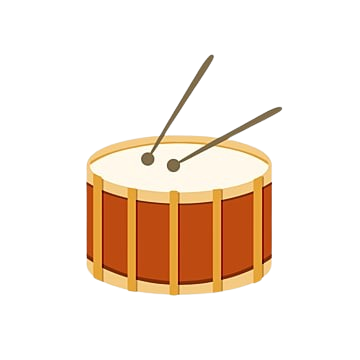
\includegraphics[width = 4 cm]{Figures/tambor2.png} 
%   %     % \caption{}
%   %     % \label{Fig. }
%   % \end{figure} 

% \end{frame}


\begin{frame}[fragile]{Sectores de la Modelación}

  % \textbf{Estudio de un sistema físico:}
  \begin{figure}[H] 
      \centering 
      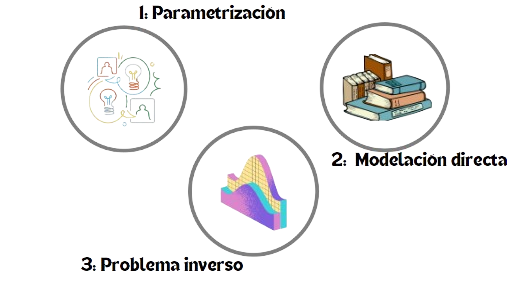
\includegraphics[width = 12 cm]{Figures/Modelos.png} 
      % \caption{}
      % \label{Fig. }
  \end{figure} 
  % \begin{enumerate}
  %     \item Parametrización del sistema: descubrimiento del conjunto mínimo de parámetros del modelo cuyos valores caracterizan completamente el sistema.
  %     \item Modelación directa (forward modeling): Descubrimiento de las leyes físicas que nos permiten hacer predicciones, dado valores de parámetros del modelo, de mediciones en observables físicas.
  %     \item Modelación inversa: Usar las mediciones de las observables físicas para inferir los valores de los parámetros del modelo.
  % \end{enumerate}

  % Los experimentos sugieren teorías físicas, y las teorías físicas predicen los resultados de los experimentos. La comparación entre la predicción y las observaciones son evidencia de la factibilidad de la teoría.
\end{frame}


\begin{frame}{Introducción}
  Abordar el problema inverso desde el enfoque bayesiano suele ser computacionalmente demandante. Por ello en este trabajo se propone un método aproximado en la solución bayesiana del problema inverso con la idea de reducir el tiempo de ejecución en las inferencias.
  
\end{frame}


\section{Antecedentes}

\begin{frame}{Modelos Descritos por ODEs}
  Consideramos modelos de la forma
  \begin{align*}
    G(t,y(t),y'(t),y''(t),...) = 0
  \end{align*}
  con $y(0)=y_0, y'(0)= y'_0, \cdots$ sus condiciones iniciales.

  Más aún, se puede generalizar a sistemas de ecuaciones diferenciales (Apostol, 2019).
\end{frame}


\begin{frame}{Forward Map}
  El \textbf{problema directo} es entonces aquel que dado un $\theta \in \Theta$ obtiene la trayectoria o solución de la ecuación diferencial.

  \vspace{1 cm}
  
  Denotemos por $\mathcal{Y}$ al espacio de las soluciones posibles de la ecuación diferencial. De esta forma existe un mapeo del espacio $\Theta$ a $\mathcal{Y}$ el cual llamaremos \textbf{forward map}. Así, el forward map es 
  \begin{align*}
      \theta \mapsto F[\theta]
  \end{align*}
  donde $\theta \in \Theta$ y $F[\theta] \in \mathcal{Y}$.
\end{frame}

\begin{frame}{Problema Inverso}

  \textbf{Ejemplo}

  \vspace{0.5 cm}

  Consideremos el siguiente modelo de la trayectoria de una partícula en un campo gravitacional
  \begin{align}
    m \ddot{x} = mg - b\dot{x},
    \label{3.1.03}
  \end{align}
  donde $x(t)$ es la trayectoria en el tiempo, $g$ la aceleración de la gravedad y $b$ el coeficiente de fricción.
  
\end{frame}

\begin{frame}{Solución Bayesiana al Problema Inverso}
  Principalmente existen dos razones para que las observaciones de un modelo no concuerden exactamente con las predicciones.

  \begin{enumerate}
    \item Errores de medición por la incertidumbre de los aparatos de medición.
    \item Defectos propios del modelo.
  \end{enumerate}
\end{frame}

\begin{frame}{Solución Bayesiana al Problema Inverso}
  El paradigma bayesiano para problemas inversos se centra en cuantificar la incertidumbre en los parámetros del modelo.
  
  Su objetivo es establecer una medida de probabilidad posterior de los parámetros del modelo dada las observaciones de la trayectoria. 
  
  Se busca la distribución de probabilidad $\pi(\theta|\mathbf{y})$ donde $\mathbf{y} = (y_1,...,y_n)$ son las observaciones de la trayectoria a lo largo del tiempo $t_1, t_2, \cdots, t_n$. 
  
  Partiendo de la información acerca de los parámetros previo a cualquier observación, se propone una distribución de probabilidad $\pi(\theta)$ llamada distribución a priori, y tras aplicar el Teorema de Bayes obtener la distribución posterior (Wasserman,2013).
\end{frame}

\begin{frame}{Cuantificación de la Incertidumbre}
  De esta forma, se establece que las discordancias entre observaciones y predicciones siguen una distribución normal de la forma
  \begin{align*}
      y_i = F_{\theta} (t_i) + \varepsilon_i, \:\:\:\:\:\: \varepsilon_i \sim N(0,\sigma^2),
  \end{align*}
  donde las $y_i's$ son las observaciones del fenómeno.
\end{frame}

\begin{frame}{Distribución Posterior}
  Se ha establecido una distribución para las observaciones $y_i$ las cuales tienen asociada una verosimilitud sobre $\theta$ y $\sigma$. Como se consideran errores condicionalmente independientes, pues se tratan de errores de medición, la verosimilitud se sigue de
  \begin{align*}
      \mathcal{L}(\theta,\sigma) &= f(\mathbf{y}|\theta,\sigma) = \prod_{i = 1}^{n} \frac{1}{\sqrt{2\pi \sigma^2}} \exp \left \{ -\frac{1}{2\sigma^2}\left(y_i - F_{\theta}(t_i)\right)^2 \right \} , 
  \end{align*}
  simplificando
  \begin{align}
      f(\mathbf{y}|\theta,\sigma) = \left(\frac{1}{2\pi \sigma^2}\right) ^{n/2}\exp \left \{  -\frac{1}{2\sigma^2}\sum_{i = 1}^{n} \left(y_i - F_{\theta}(t_i)\right)^2 \right \},
      \label{2.2.03}
  \end{align}
\end{frame}


\begin{frame}{Distribución Posterior} 
  Del teorema de Bayes, se obtiene la distribución posterior para los parámetros
  \begin{align}
      \pi(\theta | \mathbf{y})  = \frac{f(\mathbf{y}|\theta)\pi(\theta)}{\int f(\mathbf{y}|\theta)\pi(\theta)d \theta}.
      \label{2.2.04}
  \end{align}
  donde la constante de integración $h(\mathbf{y}) = \int f(\mathbf{y}|\theta)\pi(\theta)d \theta$ es la constante de normalización para la distribución posterior. 
\end{frame}

% \begin{frame}{Método MCMC}
%   Simulación de la posterior. $1/\sqrt{n}$
% \end{frame}




% \begin{frame}{Algoritmo de Metropolis-Hastings} 
%   El algoritmo de Metropolis-Hastings es un método de MCMC para generar muestras de una distribución objetivo $f(x)$ partiendo de muestras de una distribución propuesta $q(y|x)$.

%   el algoritmo de Metropolis-Hastings genera una cadena $X_0, X_1, \cdots, X_N$ construyendo recursivamente la cadena dependiendo solamente del estado previo, es decir preservando la propiedad de Markov \cite{robert1999monte}.
% \end{frame}




























% \begin{frame}{Algoritmo de Metropolis-Hastings}
%   El estado inicial $X_0$ se toma aleatoriamente. Luego, teniendo hasta el estado $X_i$, el estado $X_{i+1}$ se obtiene siguiendo 
%   \begin{enumerate}
%       \item Generar una propuesta $Y \sim q(y|X_i)$.
%       \item Calcular $\rho$ 
%       \begin{align*}
%           \rho = \min \left \{ \frac{f(y)q(x|y)}{f(x)q(y|x)}, 1  \right \} 
%       \end{align*}
%       \item Realizar un experimento Bernoulli con probabilidad de éxito $\rho$.
%       \begin{align*}
%           X_{i+1} = \left\{\begin{matrix}
%           Y & , \:\:\: \text{con probabilidad} \:\:\:\:\: \rho  \\ 
%               X_{i}&,  \text{con probabilidad} \:\:\:\:\: 1- \rho  
%             \end{matrix}\right.
%       \end{align*}
%   \end{enumerate}
% \end{frame}

% \begin{frame}{Algoritmo de Metropolis-Hastings}
%   \begin{figure}[H] 
%     \centering 
%     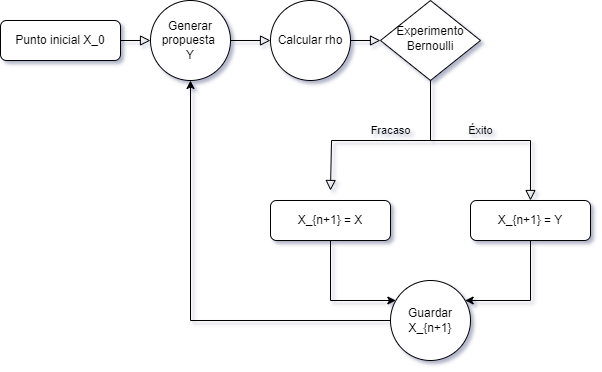
\includegraphics[width = 12 cm]{img/MCMC.png} 
%     % \caption{}
%     \label{Fig. M-H}
%   \end{figure} 
% \end{frame}

% \begin{frame}
%   Explicación punto por punto de M-H.
% \end{frame}

\begin{frame}{Forward Map Aproximado}
  
  Pensando en reducir el coste computacional.

  \begin{itemize}
    \item 
    El forward map aproximado $F_{\theta}^{*}$ es una construcción multifacética basada en aproximaciones de estadística espacial. 
    \vspace{0.5 cm}
    \item
    Tal aproximación pretende crear una distribución posterior aproximada $\tilde{\pi}(\theta|\mathbf{y})$ con la sustitución del forward map a su versión aproximada.
    \item 
    \vspace{0.5 cm}
    Existen diferentes maneras de hacer las aproximaciones del forward map. La forma propuesta es considerar una discretización del espacio de parámetros $\Theta$.
  \end{itemize}
  



\end{frame}

\begin{frame}{Construcción del Forward Map Aproximado}

  Para cada $\theta \in \Theta \subset \mathbb{R}^d$ se puede escribir como $\theta = (\theta_1, \theta_2, \cdots, \theta_d)$.

  Consideremos para cada coordenada un intervalo $[\theta_i^{min},\theta_i^{max}]$ para toda $i \in \{1,\cdots,d\}$, donde $\theta_i^{min}$ y $\theta_i^{max}$ son cotas para el espacio de parámetros que contenga la masa de probabilidad.
  
  Tomemos una partición equidistante en $M$ puntos para cada coordenada. La partición de la coordenada $i-$ésima es el conjunto $\mathcal{M}_i =\{ \theta_i^{(1)}, \theta_i^{(2)},\cdots , \theta_i^{(M-1)}, \theta_i^{(M)}\}$ con $\theta_i^{(1)} = \theta_i^{min}$ y $\theta_i^{(M)} = \theta_i^{max}$.

  De esta forma, la partición crea una malla $\mathcal{M} = \mathcal{M}_1 \times \cdots \times \mathcal{M}_d$ del espacio parametral $\Theta$.

\end{frame}

\begin{frame}{Construcción del Forward Map Aproximado}
  Sea $\vartheta \in \mathcal{M} $ elemento de la malla $\mathcal{M}$. El forward map para cada elemento de $\mathcal{M}$ es, 
  \begin{align*}
    y_j = F[\vartheta_j],
  \end{align*}
  con $y_j = y_j(t)$ funciones continuas
  
  
\end{frame}

\begin{frame}{Construcción del Forward Map Aproximado}
  Para parámetros $\theta \notin \mathcal{M}$ se propone buscar a los $k$ vectores de parámetros $\vartheta \in \mathcal{M}$ más cercanos en distancia euclidiana a $\theta$, denotando estos $k$ vecinos por $\vartheta^{(1)}, \cdots, \vartheta^{(k)}$ cada uno a una distancia $d_1, \cdots, d_k$ de $\theta$, respectivamente; con $d_1 \leq d_2 \leq \dots \leq d_k$. 
  
  \vspace{0.5 cm}

  El \textbf{forward map aproximado} con $k$ vecinos en una malla con $M$ particiones es
  \begin{align}
    \tilde{F}^{k}_M(\theta) = \sum_{j = 1}^{k} \omega_j(\theta) F \left(\vartheta^{(j)}\right)
    \label{2.4.01}
  \end{align}
  donde $\omega_j(\theta) = d_j^{-1}/ \sum_{i=1}^{k} d_i^{-1}$.
\end{frame}

\begin{frame}{Consistencia y Utilidad del Forward Map Aproximado}

  El potencial del uso del forward map aproximado para el estudio del problema inverso reside parcialmente en un menor tiempo de ejecución de la implementación en contraste con su análogo ordinario. 

  \vspace{0.5 cm}

  Existen modelos de ecuaciones diferenciales cuya implementación del problema inverso bajo enfoque bayesiano toma días en ejecutarse (Galaviz,2023).

  
\end{frame}


\begin{frame}{Consistencia y Utilidad del Forward Map Aproximado}
  Es de interés matemático el estudio de la \textbf{consistencia} del método propuesto.
  
  \vspace{0.5 cm}

  La distribución posterior aproximada para los parámetros del modelo es
  \begin{align}
    \tilde{\pi}^{k}_M(\theta|\mathbf{y}) \propto \left(\frac{1}{2\pi \sigma^2}\right) ^{n/2}\exp \left \{  -\frac{1}{2\sigma^2}\sum_{i = 1}^{n} \left(y_i - F^k_M(\theta)\right)^2 \right \}\pi(\theta),
    \label{2.4.02}
  \end{align}
\end{frame}

\begin{frame}{Consistencia y Utilidad del Forward Map Aproximado}

  Para formalizar la consistencia del forward map  aproximado se hace uso de la \textit{distancia de Kullback-Leibler}.

  La distancia de Kullback-Leibler entre $f$ y $g$ se define como
  \begin{align*}
      D(f,g) = \int f(x)\log \left(\frac{f(x)}{g(x)}\right) dx.
  \end{align*}

  Se puede mostrar que $D(f,g) \geq 0$ y $D(f,f) = 0$ (Wasserman,2006).

\end{frame}

\begin{frame}{Consistencia y Utilidad del Forward Map Aproximado}
  Definamos la distancia entre las distribuciones posteriores como
  \begin{align*}
      c^k_M = D \left( \pi(\theta|\mathbf{y}),\tilde{\pi}^{k}_M(\theta|\mathbf{y})\right)
  \end{align*}

  Diremos que el forward map aproximado es \textbf{consistente} si para una cantidad de vecinos $k$ fijo y conocido, las distancias 
  \begin{align*}
      c^k_M \rightarrow 0 \:\:\:\:\:\: \text{a medida que}\:\:\:\:\:\: M \rightarrow \infty
  \end{align*}
\end{frame}



\begin{frame}{Consistencia y Utilidad del Forward Map Aproximado}
  La consistencia en el caso $k=1$ se tiene de (\ref{2.4.01})
  \begin{align*}
    \tilde{F}^{k}_M(\theta) = \sum_{j = 1}^{k} \omega_j(\theta) F \left(\vartheta^{(j)}\right)
  \end{align*}
  donde $\omega_j(\theta) = d_j^{-1}/ \sum_{i=1}^{k} d_i^{-1}$.

  \vspace{0.5 cm}

  Se requieren hipótesis extras.
\end{frame}

\section{Implementación}

\begin{frame}{Implementación}

  Se ha optado por un desarrollo heurístico centrado en \textbf{experimentación} con una variedad de parámetros o indicadores estratégicamente seleccionados.

  \vspace{0.5 cm}

  Se consideran tres modelos en ecuaciones diferenciales, de los cuales se describen a continuación.
\end{frame}


\begin{frame}{Modelo Gravitatorio}
  Consideremos una partícula puntual en un campo gravitatorio. La mecánica clásica modela la dinámica con la ecuación diferencial
  \begin{align}
    m \ddot{x} = mg - b\dot{x},
    \label{3.1.03}
  \end{align}
  donde $x(t)$ es la trayectoria en el tiempo, $g$ la aceleración de la gravedad y $b$ el coeficiente de fricción.

  La solución explicita es
  \begin{align}
    x(t) = v_T \left [ t - \frac{m}{b} \left( 1- \exp\left\{-\frac{b}{m} t\right\}\right)\right],
    \label{3.1.12}
  \end{align}
  Con $\dot{x}(0)=0$ y $x(0) = 0$.
\end{frame}


\begin{frame}{Modelo Gravitatorio}
  \begin{figure}
    \centering
    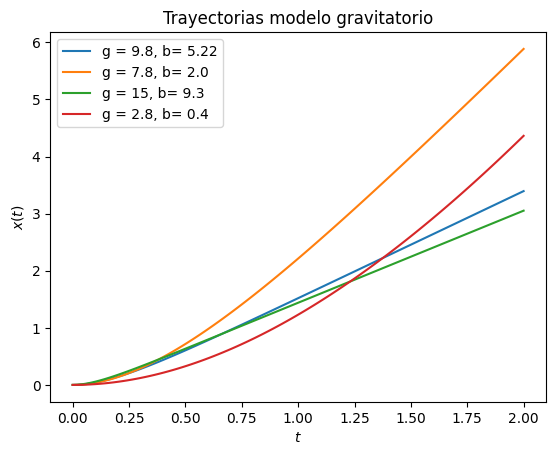
\includegraphics[width = 9 cm]{img/Trayectoria.png}
    % \caption{Varias trayectorias con la dinámica gravitación sujeta a fricción para varias valores de los parámetros g,b.}
    \label{fig:trayectoria_gravedad}
  \end{figure}
\end{frame}

\begin{frame}{Modelo Logístico}
  El modelo que describe el tamaño de una población $P(t)$ con recursos finitos se describe por medio del modelo logístico. 
  \begin{align}
    \frac{dP}{dt} = rP\left(1- \frac{P}{K}  \right),
    \label{3.1.2.03}
  \end{align}
  donde $r$ es la tasa de crecimiento y $K$ la capacidad de sustento.
  
  Con $P(0) = P_0$, la solución explicita es
  \begin{align}
      P(t) = \frac{KP_0 e^{rt}}{K + P_0 \left(e^{rt}-1\right)},    
      \label{3.1.2.05}
  \end{align}
  donde verificamos que $\lim_{t \rightarrow \infty}P(t) = K $. 
\end{frame}

\begin{frame}{Modelo Logístico}
  \begin{figure}
    \centering
    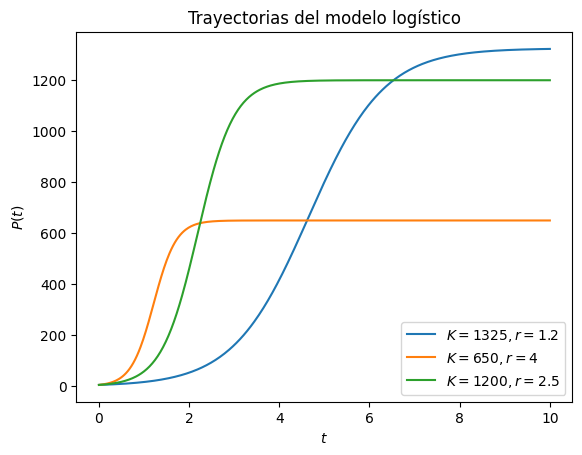
\includegraphics[width = 9 cm]{img/trayectoria_log.png}
    % \caption{Varias trayectorias con la dinámica de crecimiento logístico para varias valores de los parámetros K,r.}
    \label{fig:trayectoria_logistico}
  \end{figure}
\end{frame}

\begin{frame}{Modelo Logístico}
  Existe otra reparametrización del modelo logístico de la forma
  \begin{align}
    \frac{dX(t)}{dt} = \theta_1 X(t)\left(\theta_2 - X(t)\right).
    \label{3.1.2.06}
  \end{align}

  Con la parametrización dada por
  \begin{align*}
      \theta_1 = \frac{r}{K}, \:\:\:\:\:\: \theta_2 = K,
  \end{align*}
  recuperamos la expresión dada en (\ref{3.1.2.03}).

\end{frame}


\begin{frame}{Modelo SIR}

  Modelo epidemiológico que divide la población en clases:
  \begin{enumerate}
    \item Susceptible ($S$): Cantidad de personas que no han tenido la enfermedad ni están enfermas del brote de interés.
    \item Infeccioso ($I$): Son las personas que actualmente portan el patógeno y son además un vector de transmisión.
    \item Recuperado ($R$): Para aquellas personas que se han recuperado de la enfermedad y ya tienen inmunidad o también para aquellas que perecieron.
  \end{enumerate}
  
\end{frame}


\begin{frame}{Modelo SIR}
  La dinámica del modelo SIR se da con el siguiente sistema de EDO's
  \begin{align}
      \frac{dS}{dt} &= -\beta S I, \nonumber \\
      \frac{dI}{dt} &= \beta S I - \gamma I,
      \label{3.1.3.01} \\
      \frac{dR}{dt} &= \gamma I, \nonumber
  \end{align}
  donde $\beta$ es la tasa de infección, $\gamma$ es la tasa de recuperación y $S + I + R = N$ (Weiss,2013).
\end{frame}

\begin{frame}{Modelo SIR}
  \begin{figure}
    \centering
    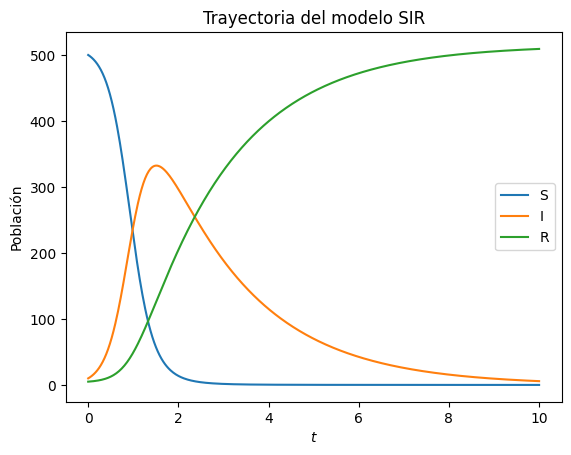
\includegraphics[width = 9 cm]{img/trayectoria_SIR.png}
    % \caption{Trayectoria de cada grupo del modelo SIR con $\beta = 0.009$ y $\gamma = 0.5$.}
    \label{fig:trayectoria_SIR}
  \end{figure}
\end{frame}

\begin{frame}{Enfoque Bayesiano al Problema Inverso}
  Nos enfocamos en abordar el problema inverso para los modelos descritos.

  La muestra $y_1, y_2, \cdots, y_n$ se obtiene de \textbf{simulación}. 
  \begin{enumerate}
    \item 
    Tomamos $\theta \in \Theta$ fijo.
    \item
    Consideramos los tiempos a los cuales corresponderá la muestra, denotados por $t_1, t_2, \cdots, t_n$. 
    \item
    Agregamos un ruido $\varepsilon_i \sim N(0,\sigma^2)$.
    \begin{align}
      y_i = F_{\theta}(t_i) + \varepsilon_i.
      \label{3.2.01}
    \end{align}
  \end{enumerate}
  
\end{frame}


\begin{frame}{Enfoque Bayesiano al Problema Inverso}
  El problema inverso busca $\theta$ tal que $y_i \approx F_{\theta}(t_i)$.

  \vspace{0.5 cm}

  En la teoría de la estadística bayesiana, el paradigma central se basa en obtener la distribución posterior de los parámetros de interés dada las observaciones.
  \begin{align}
    \pi(\theta|\mathbf{y}) \propto f(\mathbf{y}|\theta) \pi(\theta).
    \label{3.2.1.01}
  \end{align}
  De la verosimilitud en (\ref{2.2.03})
  \begin{align}
    \pi(\theta|\mathbf{y}) \propto \left(\frac{1}{2\pi \sigma^2}\right) ^{n/2}\exp \left \{  -\frac{1}{2\sigma^2}\sum_{i = 1}^{n} \left(y_i - F_{\theta}(t_i)\right)^2 \right \} \pi(\theta),
    \label{3.2.1.02}
  \end{align}
\end{frame}

\begin{frame}{Enfoque Bayesiano al Problema Inverso}

  Se proponen distribuciones a priori gamma
  \begin{align}
    \theta_i \sim Gamma\left(\alpha_i, \frac{\theta_i^{*}}{\alpha_i} \right),
    \label{3.2.1.03}
  \end{align}
  con $\theta_i^{*}$ y $\alpha_i$ parámetros conocidos.
  
  Como $\theta_i$ se proponen condicionalmente independientes, entonces la distribución a priori para $\theta$ es
  \begin{align}
    \pi(\theta|\alpha) &= \pi(\theta_1|\alpha_1) \cdots \pi(\theta_d|\alpha_d)
    \label{3.2.1.04}
  \end{align}
  
  \vspace{0.5 cm}

  La parametrización de la $Gamma(\alpha,\beta)$ es tal que su función de densidad sea
  \begin{align*}
    f(\theta|\alpha,\beta) = \frac{\beta^\alpha}{\Gamma(\alpha)} \theta^{\alpha-1} \exp \left \{ -\beta \theta\right \},
  \end{align*}
\end{frame}

\begin{frame}{Enfoque Bayesiano al Problema Inverso}
  Salvo un factor, la distribución posterior es 
  \begin{align}
    &\pi(\theta, \sigma|\mathbf{y}) \propto  \nonumber\\ &\left(\frac{1}{2\pi \sigma^2}\right) ^{n/2}\exp \left \{  -\frac{1}{2\sigma^2}\sum_{i = 1}^{n} \left(y_i - F_{\theta}(t_i)\right)^2 \right \} \prod_{i = 1}^{n} \left[\frac{1}{\Gamma(\alpha_i)}\left(\frac{\theta_i^{*}}{\alpha_i}\right) ^{\alpha_i} \theta_i^{\alpha_i -1} \exp \left \{ -\frac{\theta_i^{*}}{\alpha_i}\theta_i\right \}\right] 
    \label{3.2.1.06}
  \end{align}
\end{frame}

\begin{frame}{Enfoque Bayesiano al Problema Inverso}
  Usando MCMC obtenemos una muestra de la distribución posterior $(X_i, i \in \{1,\cdots, T\})$.

  En beneficio de la ley de grandes números, la media 
  \begin{align}
    \mathbb{E}\left [X\right ] \approx \frac{1}{T}\sum_{i = 1}^{T} X_i
  \end{align}
  Para la media del estadístico $h(X)$ 
  \begin{align}
    \mathbb{E}\left [h(X)\right ] \approx \frac{1}{T} \sum_{i=1}^{T} h(X_i)
    \label{3.2.2.01}
  \end{align}

\end{frame}

\begin{frame}{Simulación del Modelo Gravitatorio}
  El Forward map para el modelo gravitatorio es $F[\theta](t) = F[g,b] (t)= x(t)$ con $x_0 = 0$ y $v_0 = 0$

  Consideremos las distribuciones a priori (\ref{3.2.1.03}) como
  \begin{align}
    g \sim Gamma \left(\alpha, \frac{\theta_1^{*}}{\alpha}\right) \\
    b \sim Gamma \left(\beta, \frac{\theta_2^{*}}{\beta}\right) 
  \end{align}
  
\end{frame}

\begin{frame}{Simulación del Modelo Gravitatorio}
  
\begin{figure} 
  \centering 
  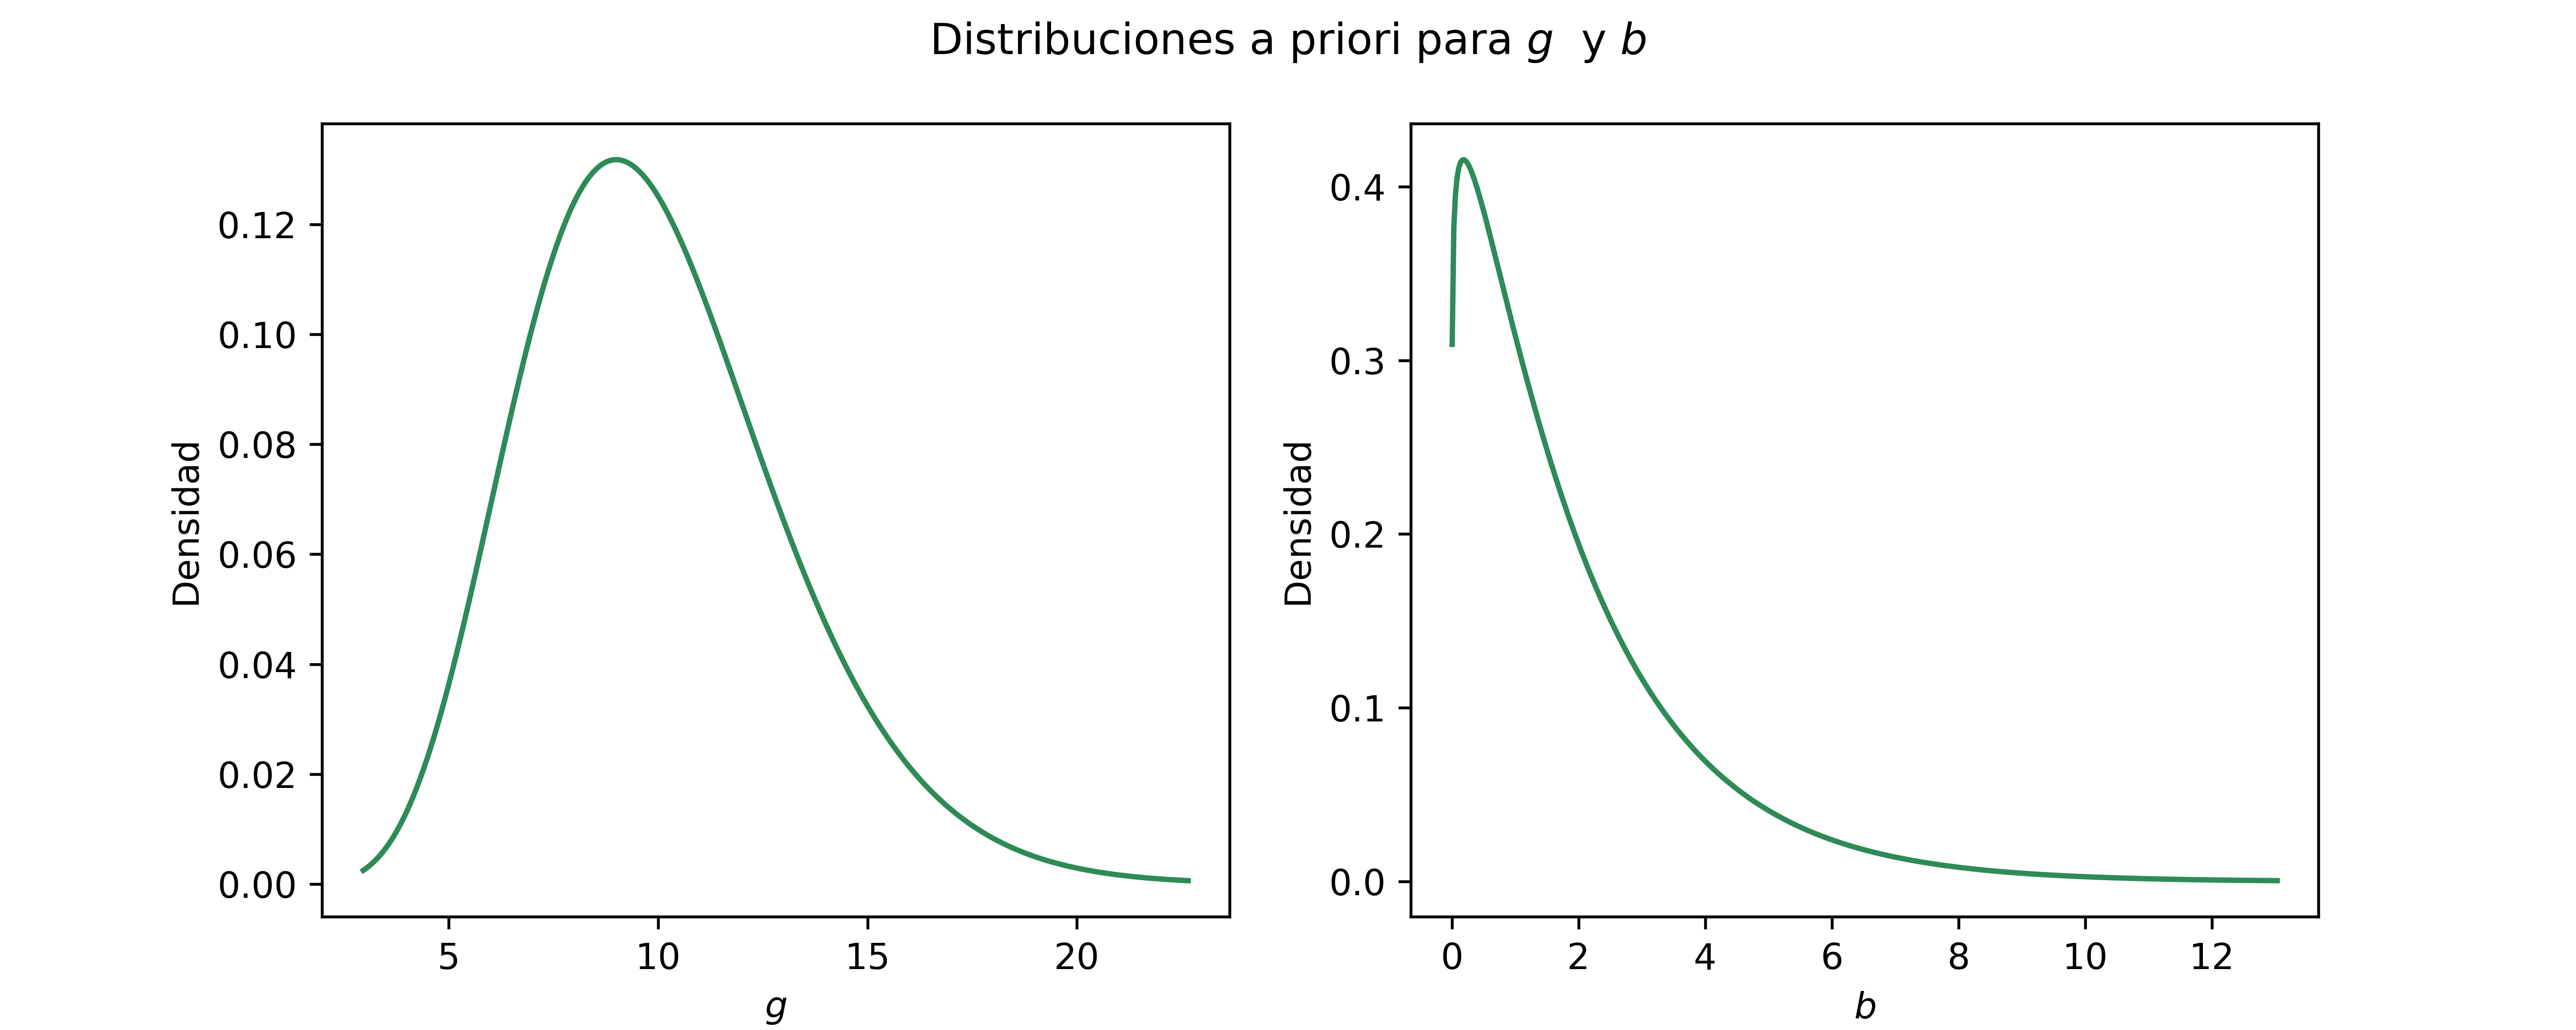
\includegraphics[width = 15 cm]{img/Exp_Central_gravedad_sigma/Figuras/Generales/Apriori_gravedad_sigma.png}
  % \caption{Distribuciones marginal a priori para el parámetro $g$ (izquierda) y $b$ (derecha).}
  \label{Fig. 3.2.2.01}
  \end{figure} 
\end{frame}

\begin{frame}{Simulación del Modelo Gravitatorio}
  
  \begin{figure}
    \centering 
    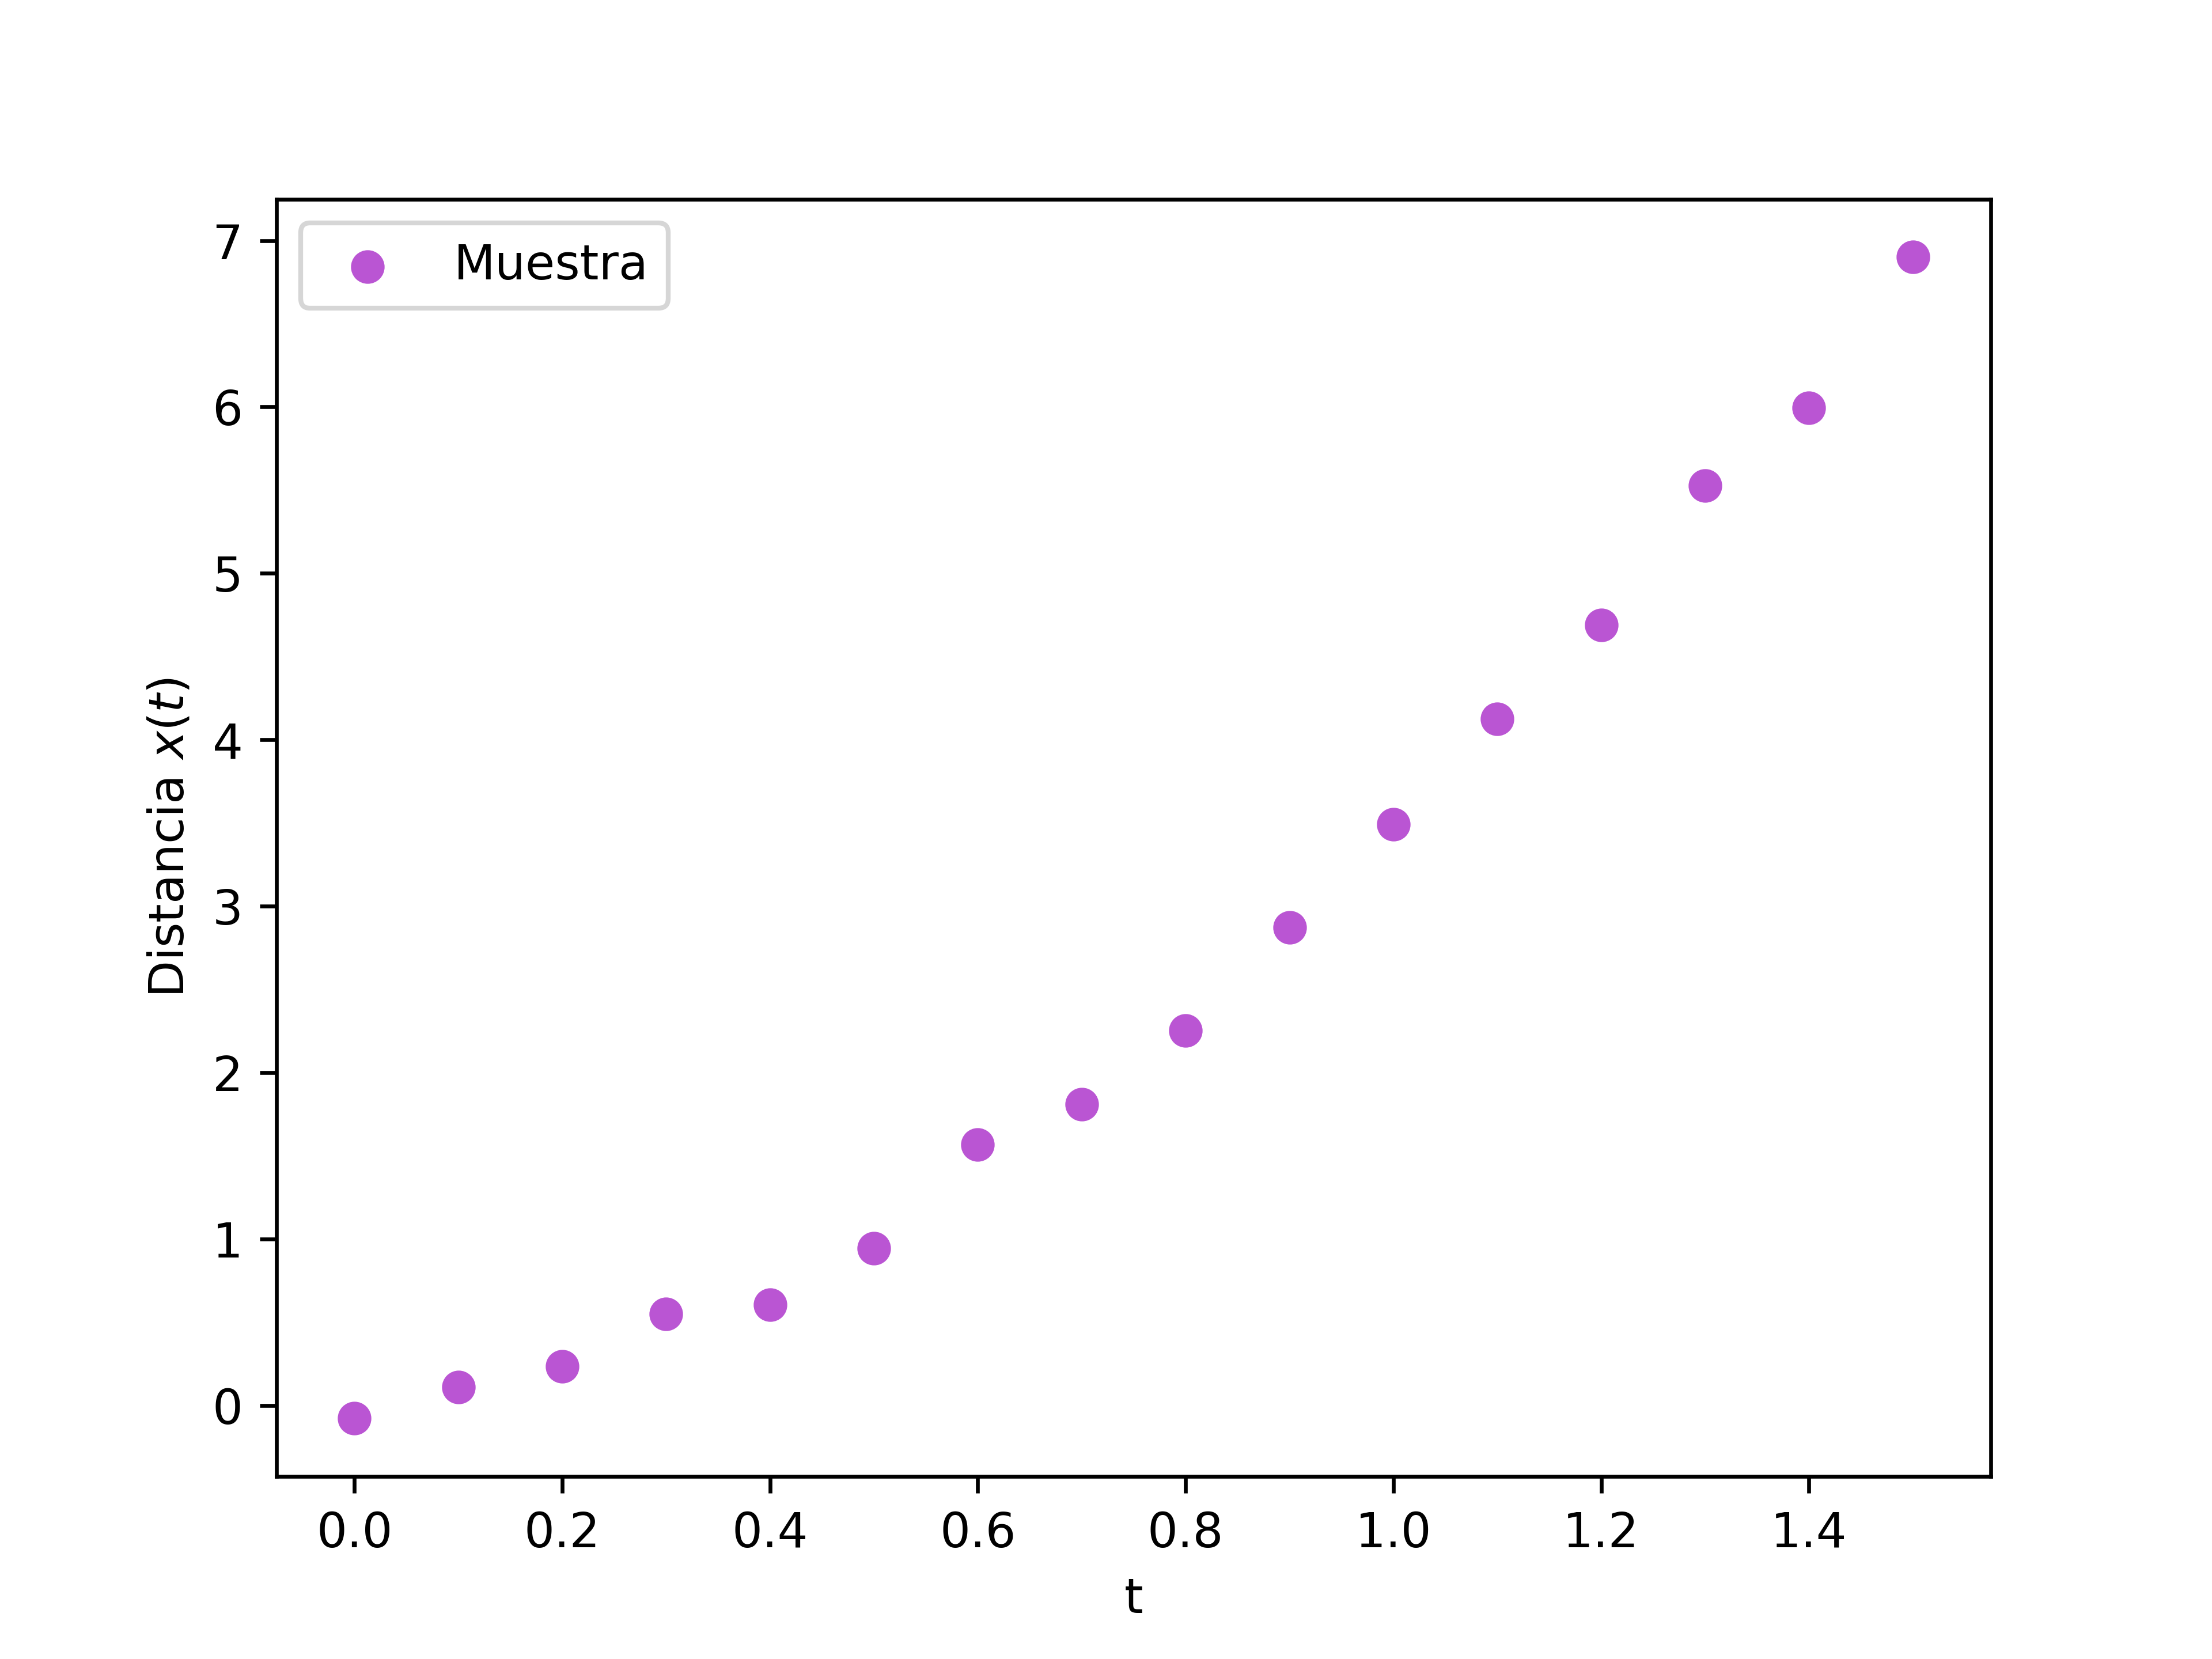
\includegraphics[width = 9 cm ]{img/Exp_Central_gravedad_sigma/Figuras/Generales/Muestra_gravedad_sigma.png} 
    % \caption{Muestra $\mathbf{y}$ del modelo gravitatorio.}
    \label{Fig. 3.2.2.02}
  \end{figure} 
\end{frame}

\begin{frame}{Simulación del Modelo Gravitatorio}
  Considerando un MCMC de $T = 600,000$ iteraciones y un burn in de $20,000$ \cite{christen2010general}. 
\end{frame}

\begin{frame}{Simulación del Modelo Gravitatorio}
  \begin{figure}
    \centering 
    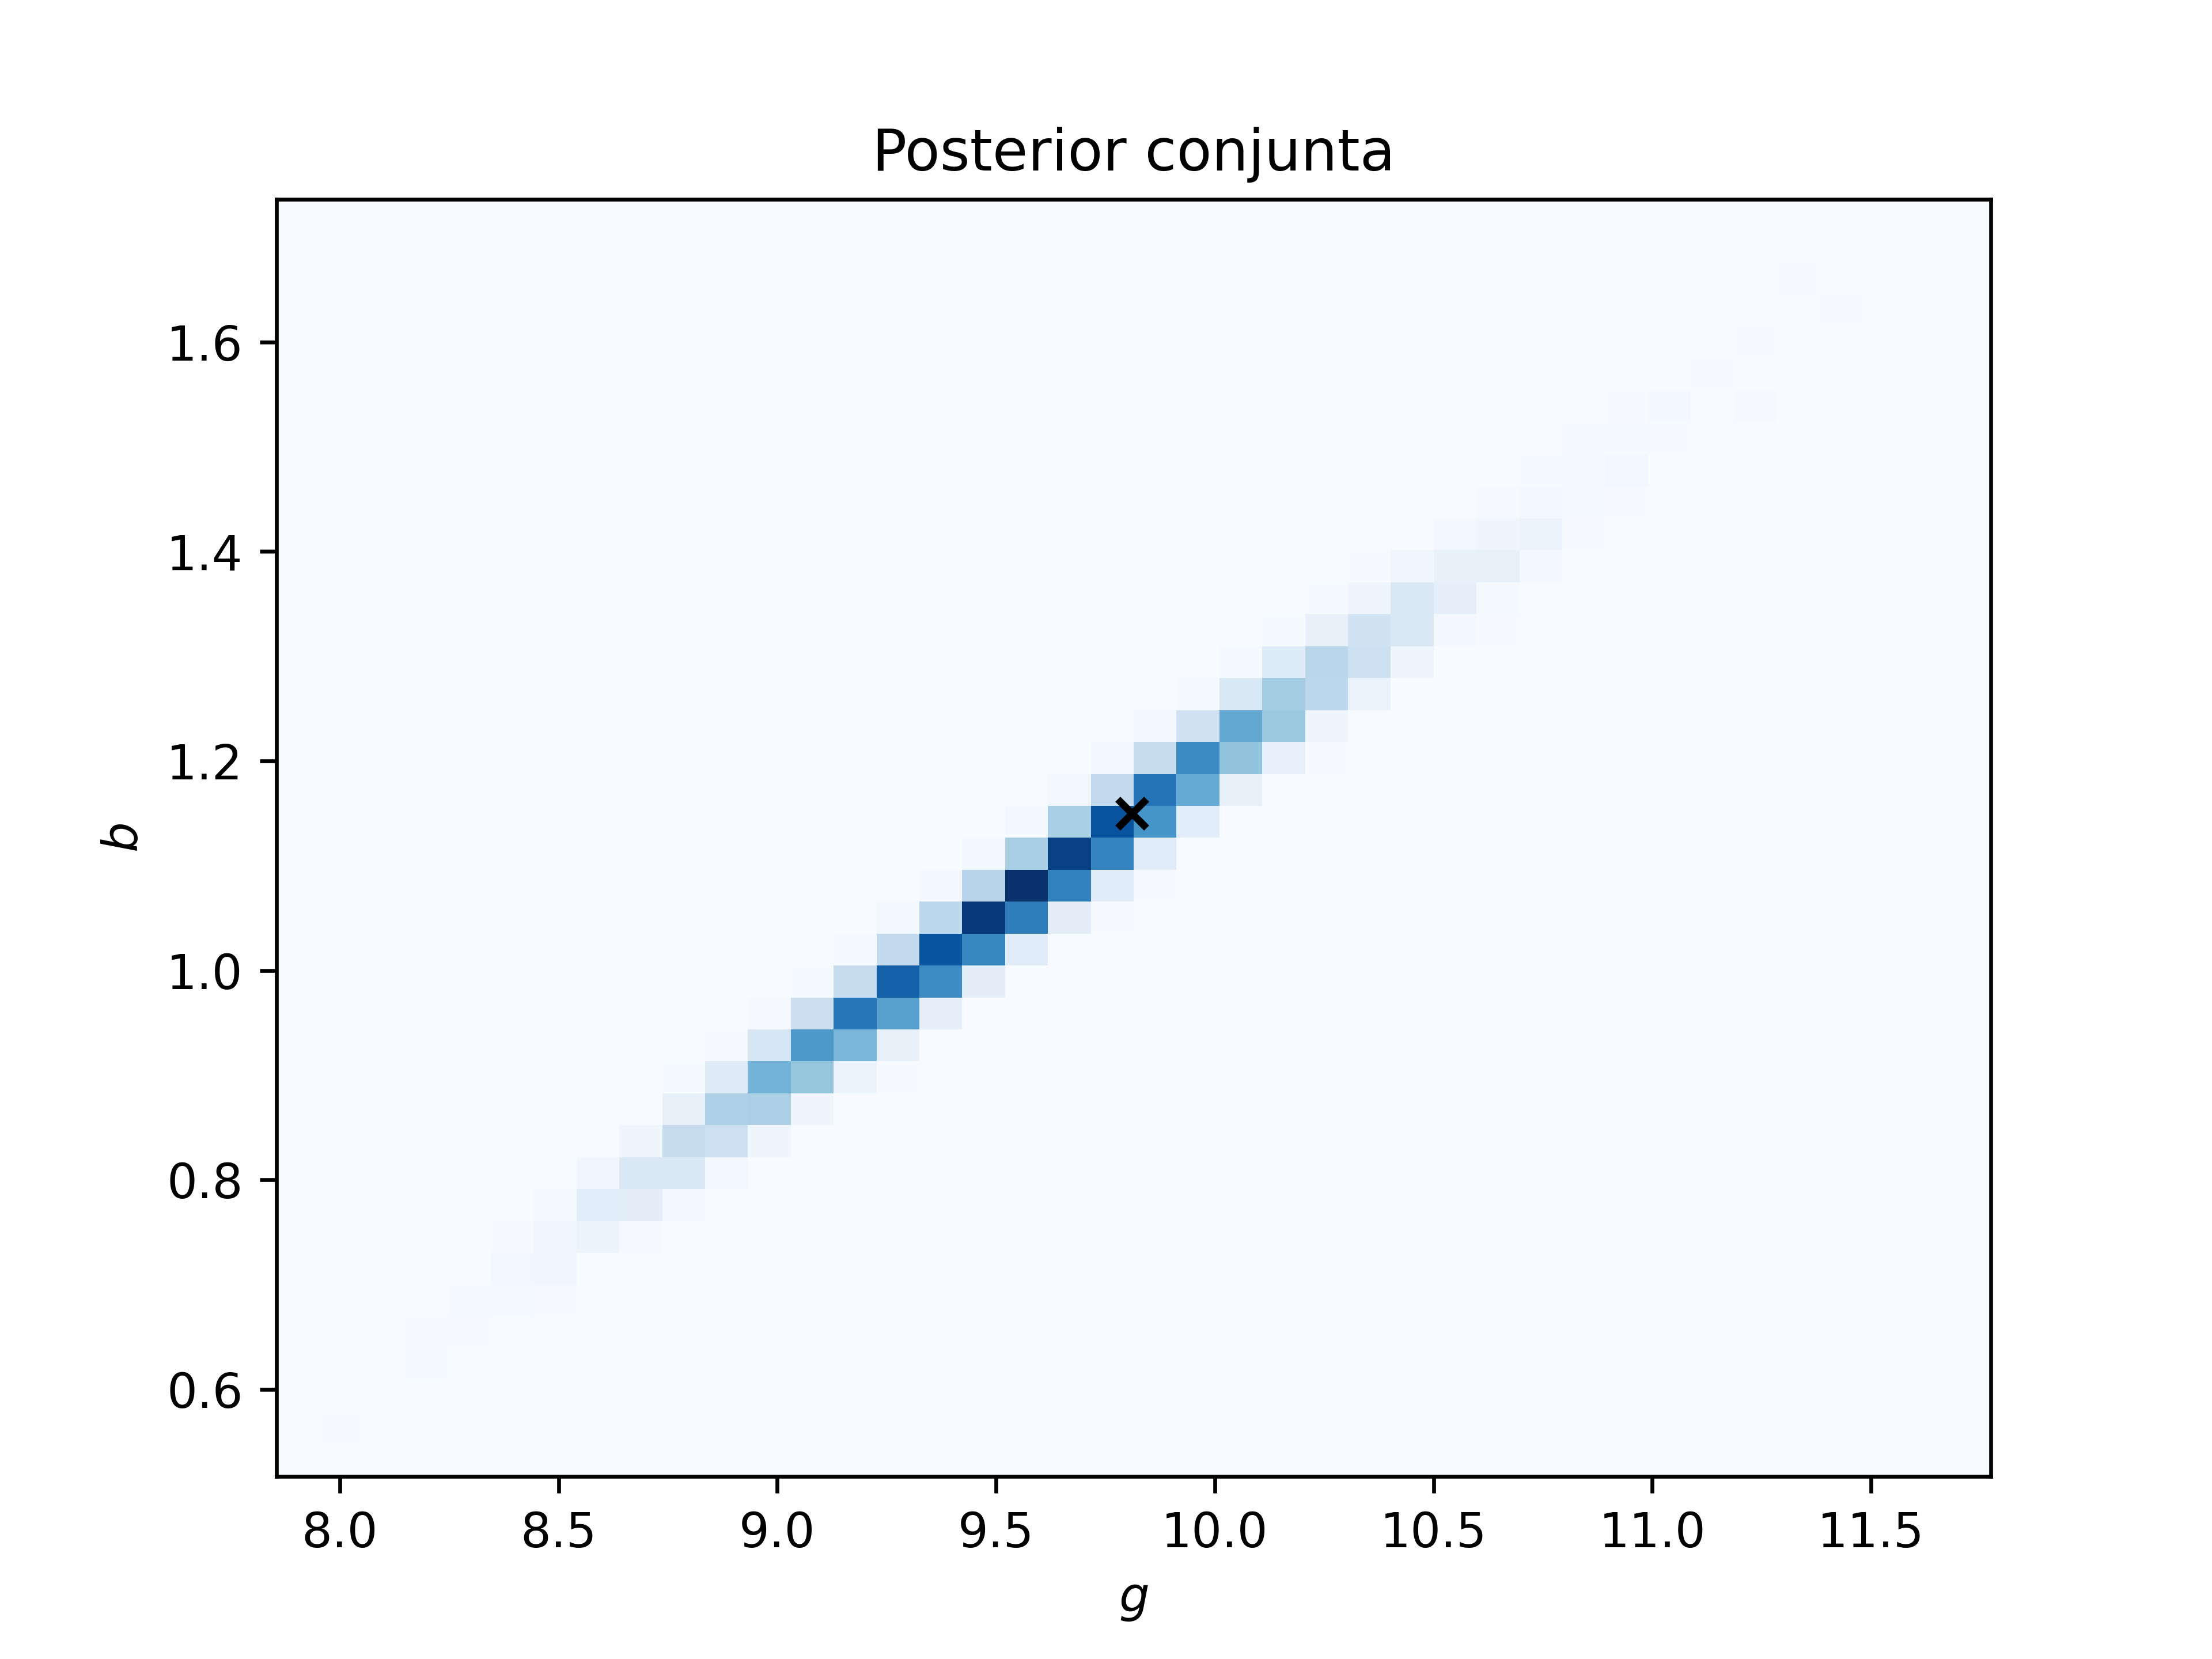
\includegraphics[width = 9 cm ]{img/Exp_Central_gravedad_sigma/Figuras/Generales/Conjunta_gravedad_sigma.png} 
    % \caption{Estimación de la distribución posterior conjunta por método MCMC Metropolis-Hastings.}
    \label{Fig. 3.2.2.03}
  \end{figure} 
\end{frame}

\begin{frame}{Simulación del Modelo Gravitatorio}
  \begin{columns}[T,onlytextwidth]
    \column{0.5\textwidth}

    \begin{figure}
      \centering 
      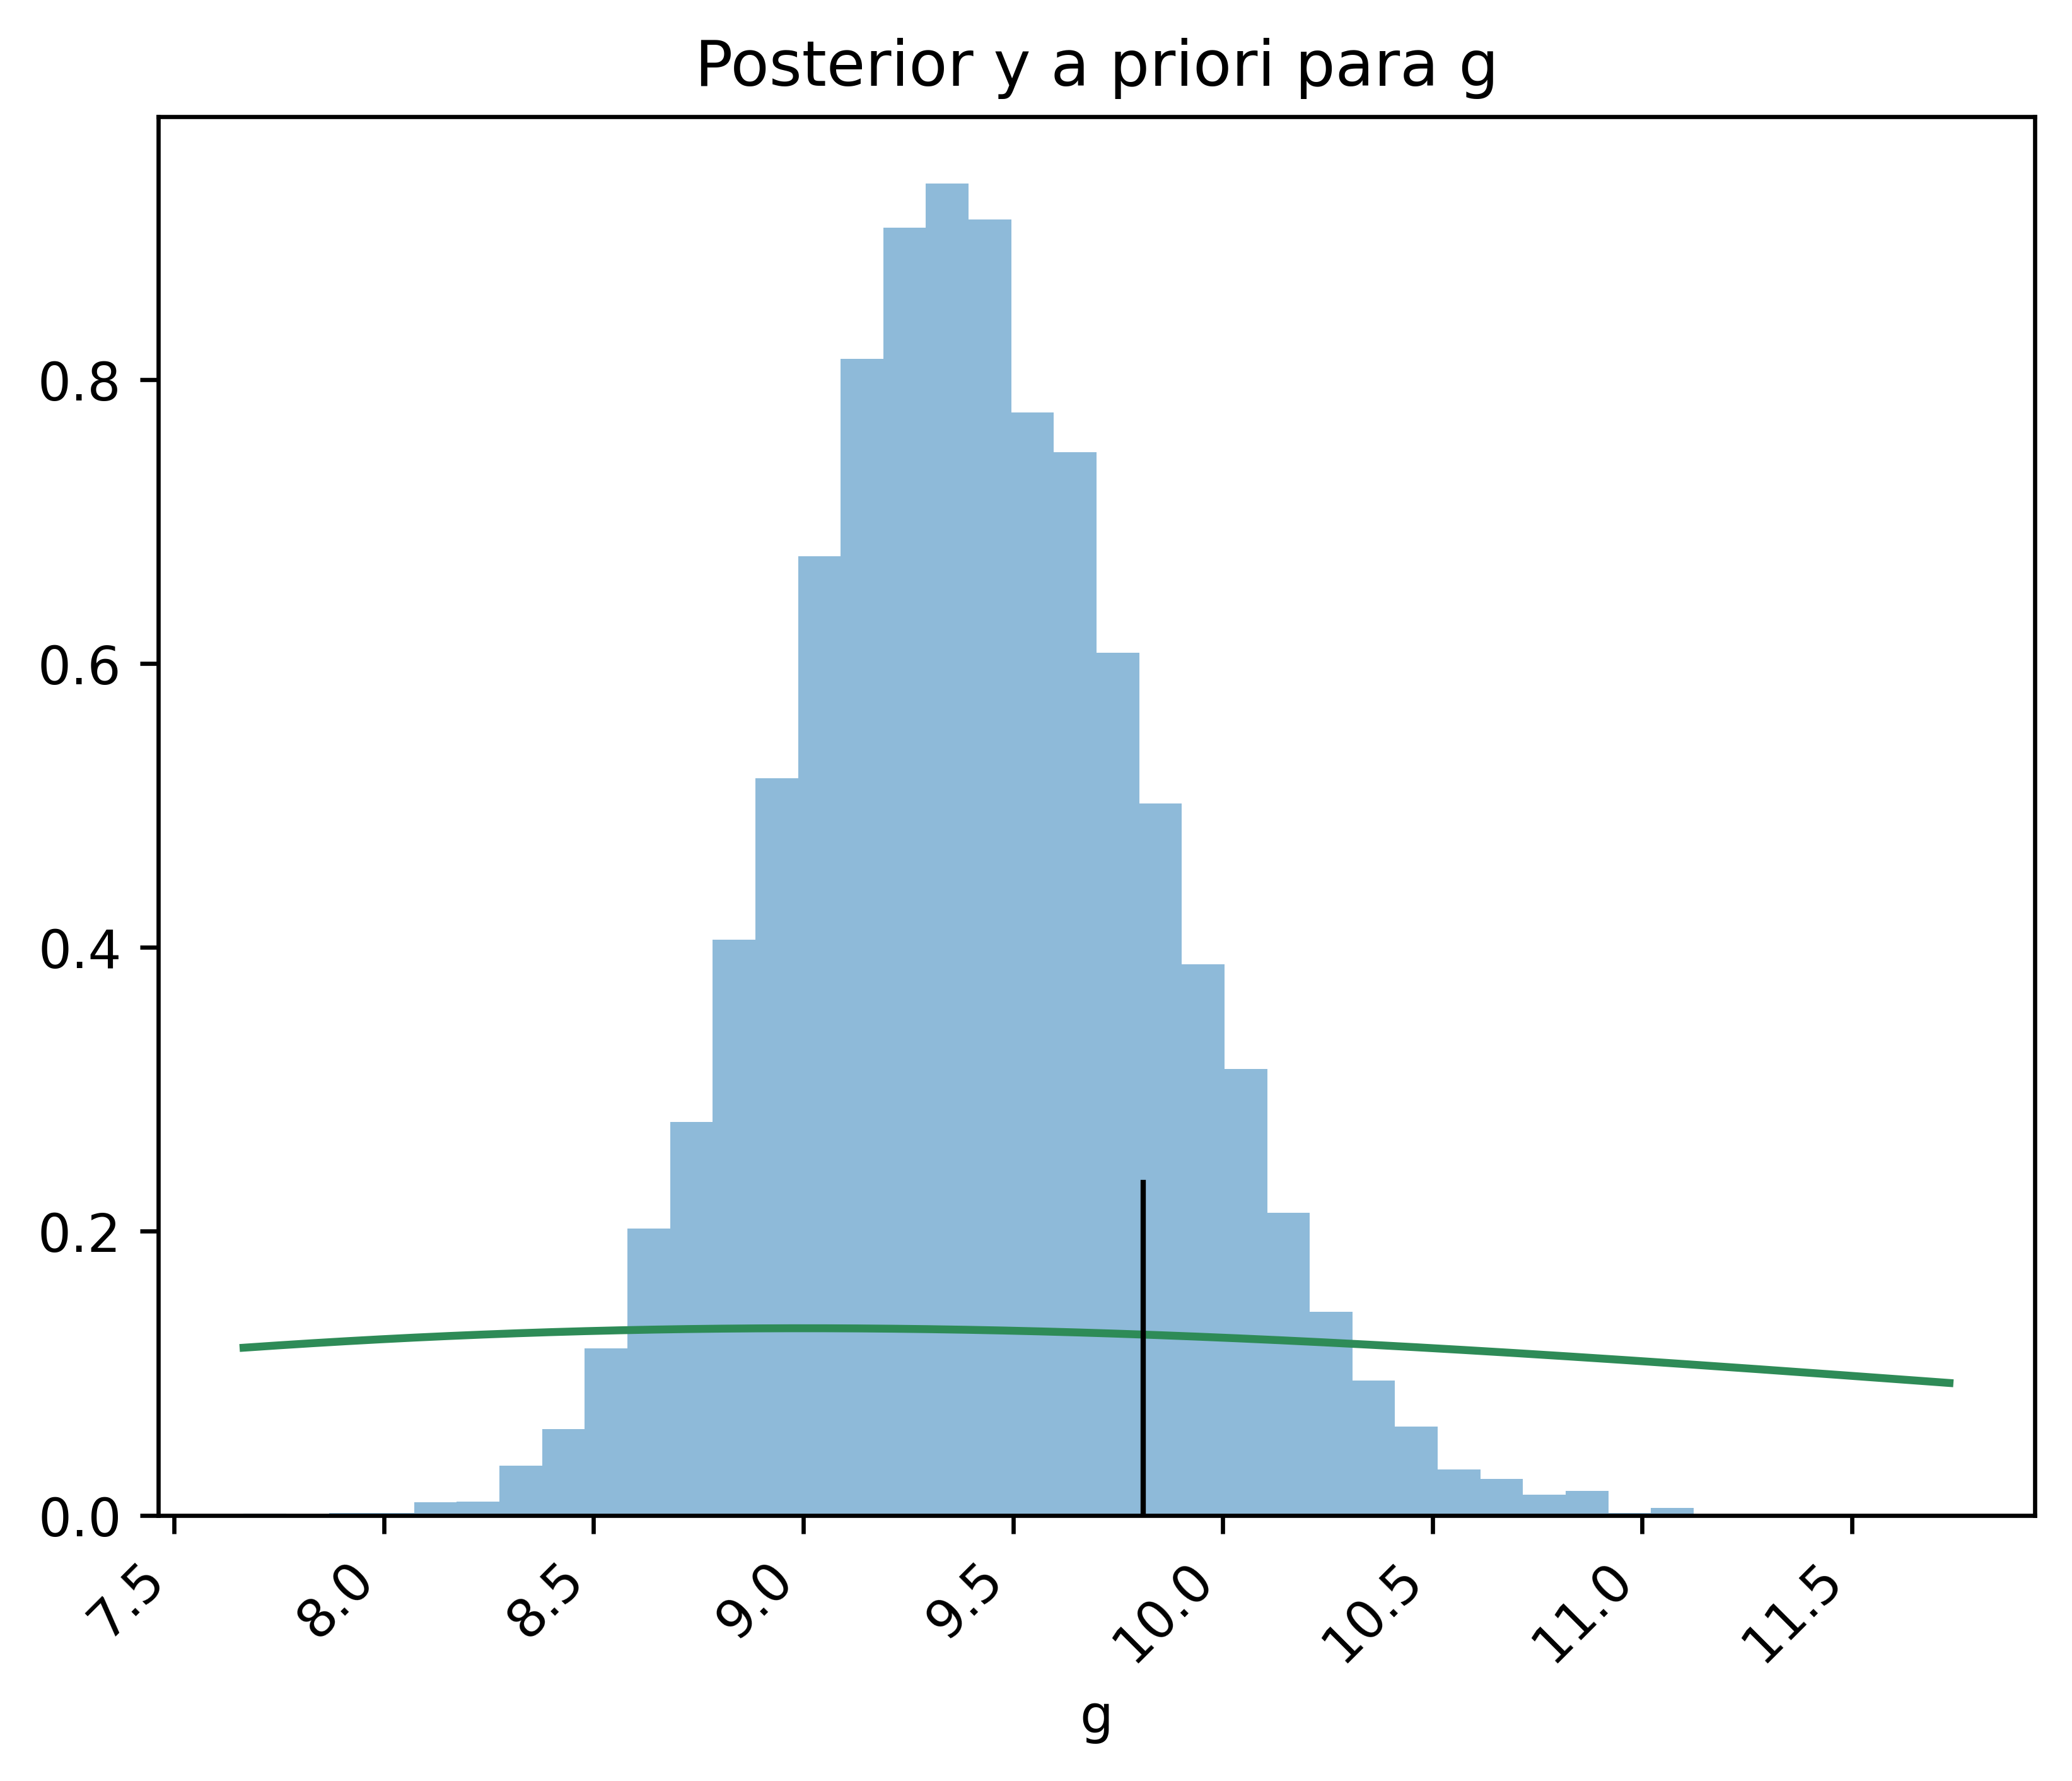
\includegraphics[width=0.9\textwidth]{img/Exp_Central_gravedad_sigma/Figuras/Generales/Post_theta1_gravedad_sigma.png}
    \end{figure} 
    
    \column{0.5\textwidth}

      % \metroset{block=fill}

    \begin{figure}
      \centering 
      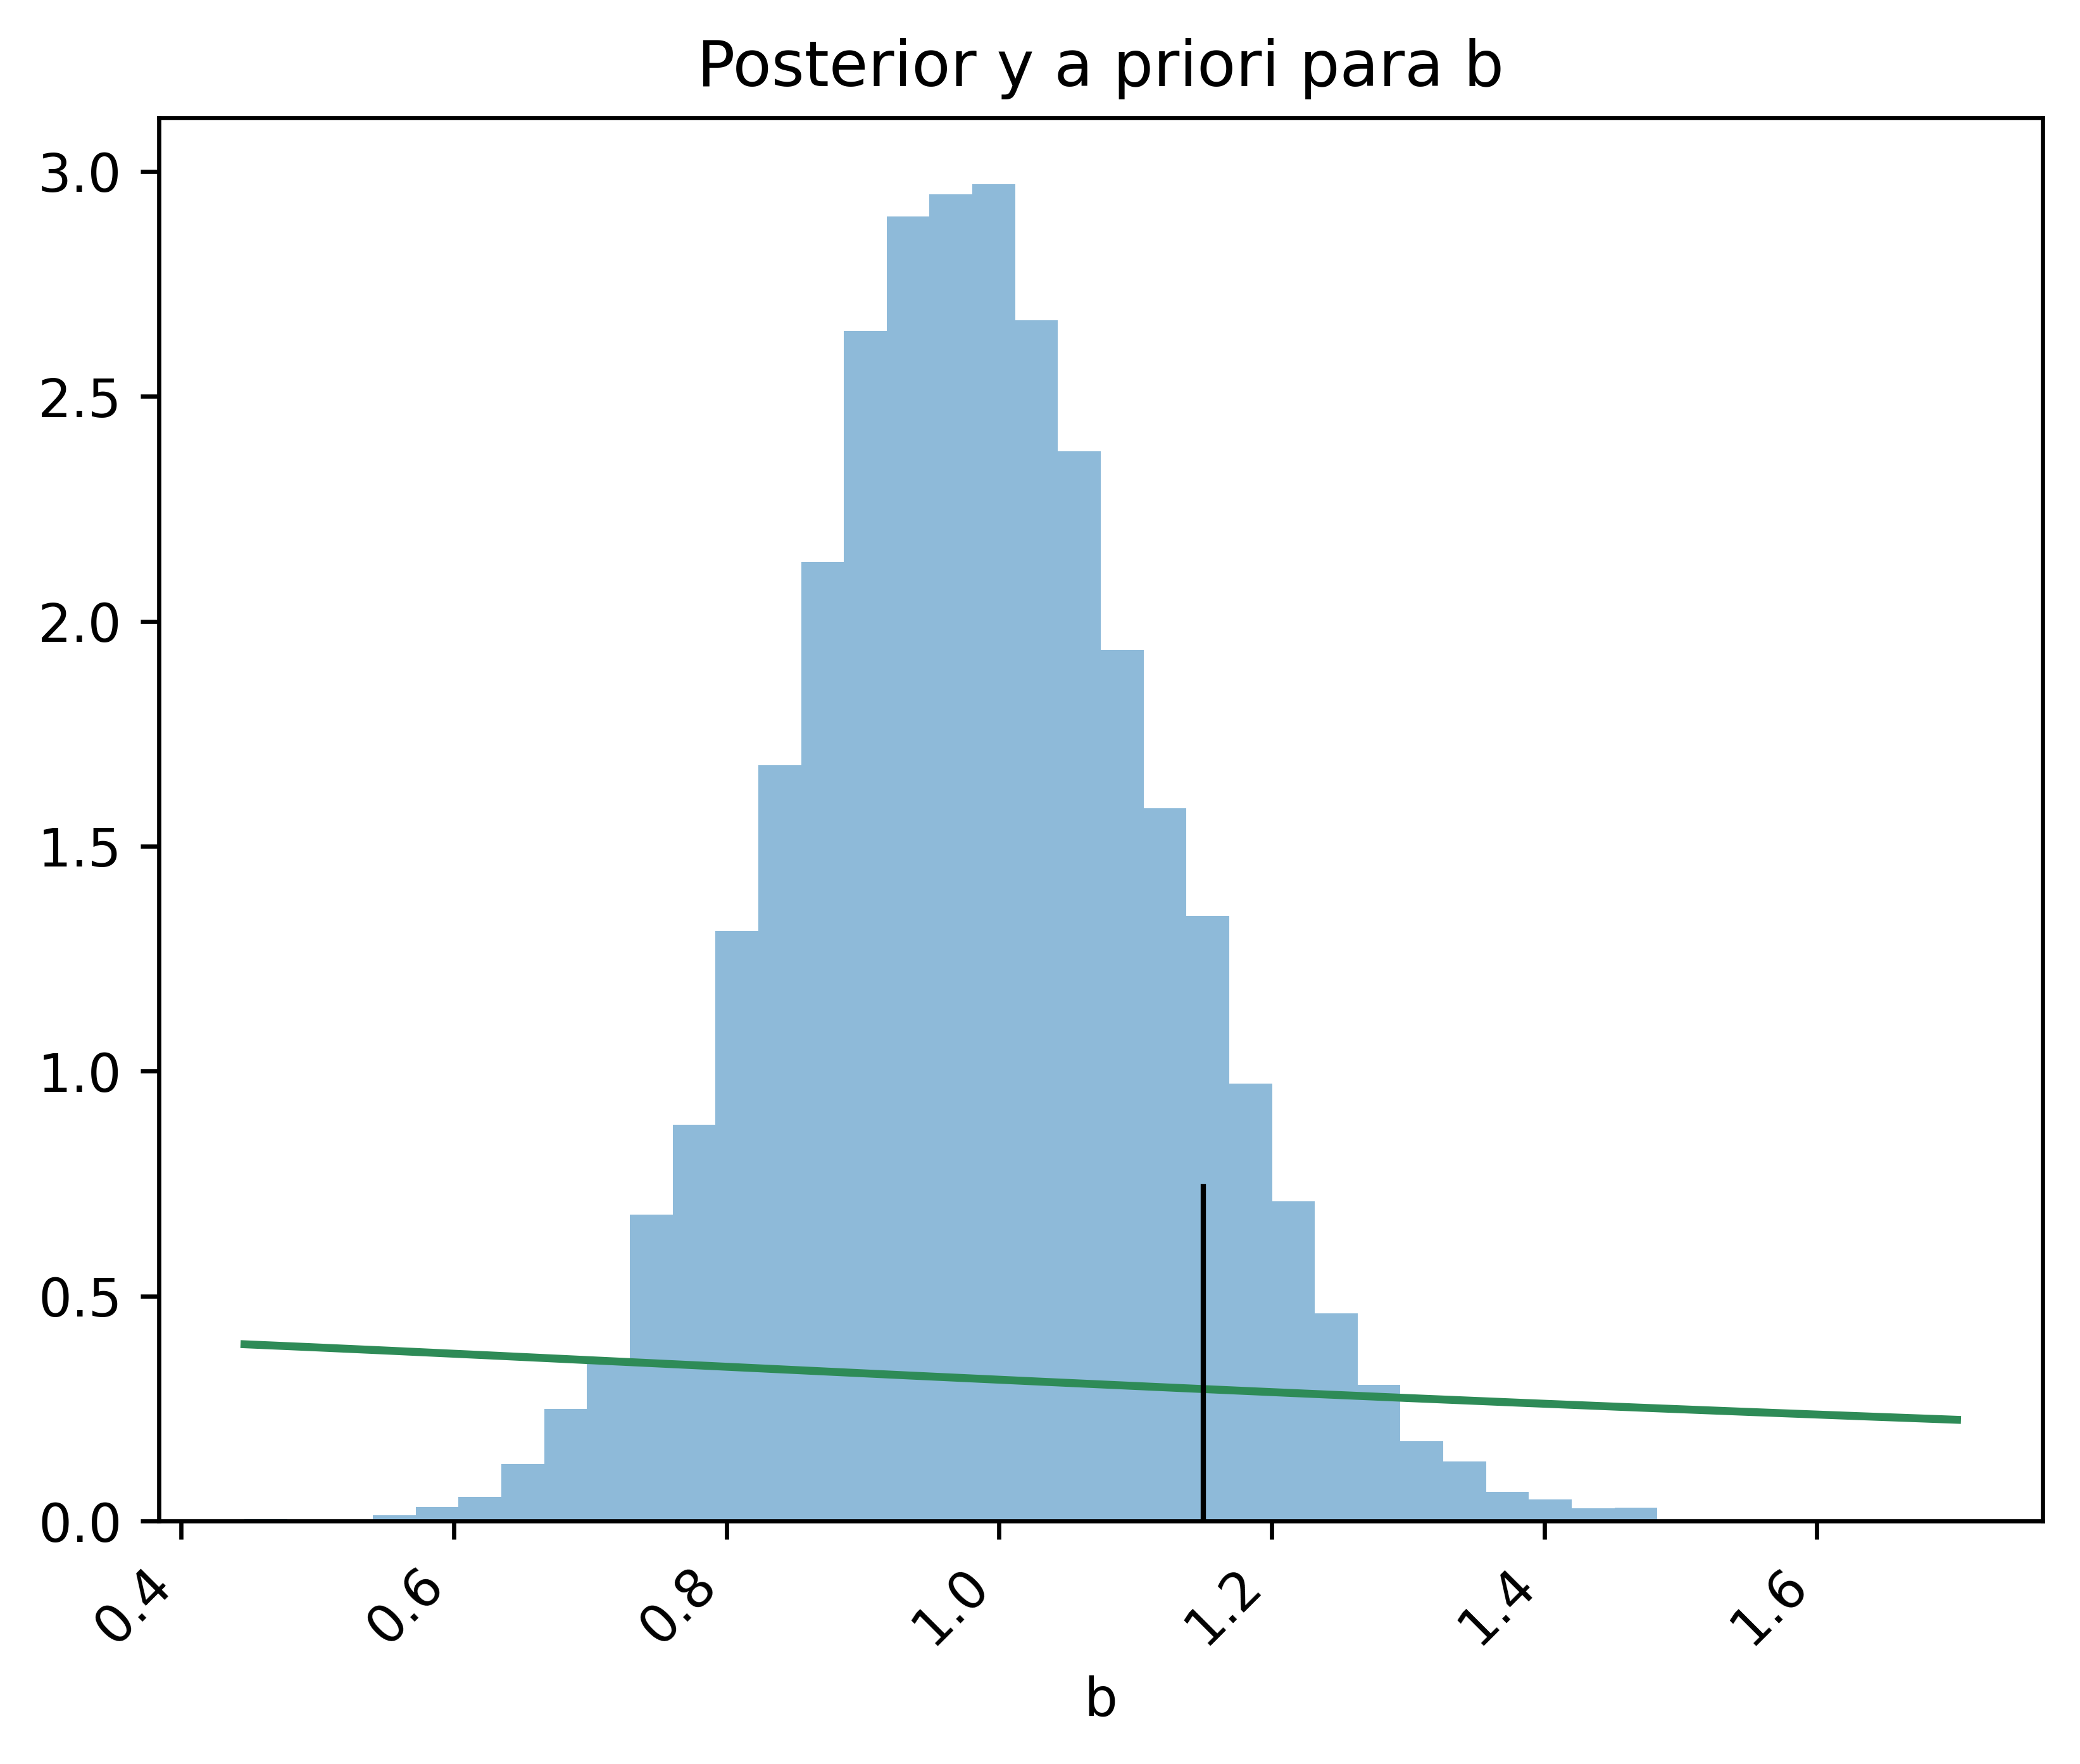
\includegraphics[width=0.9\textwidth]{img/Exp_Central_gravedad_sigma/Figuras/Generales/Post_theta2_gravedad_sigma.png}
    \end{figure} 

  \end{columns}
\end{frame}

\begin{frame}{Simulación del Modelo Gravitatorio}
  \begin{figure}
    \centering 
    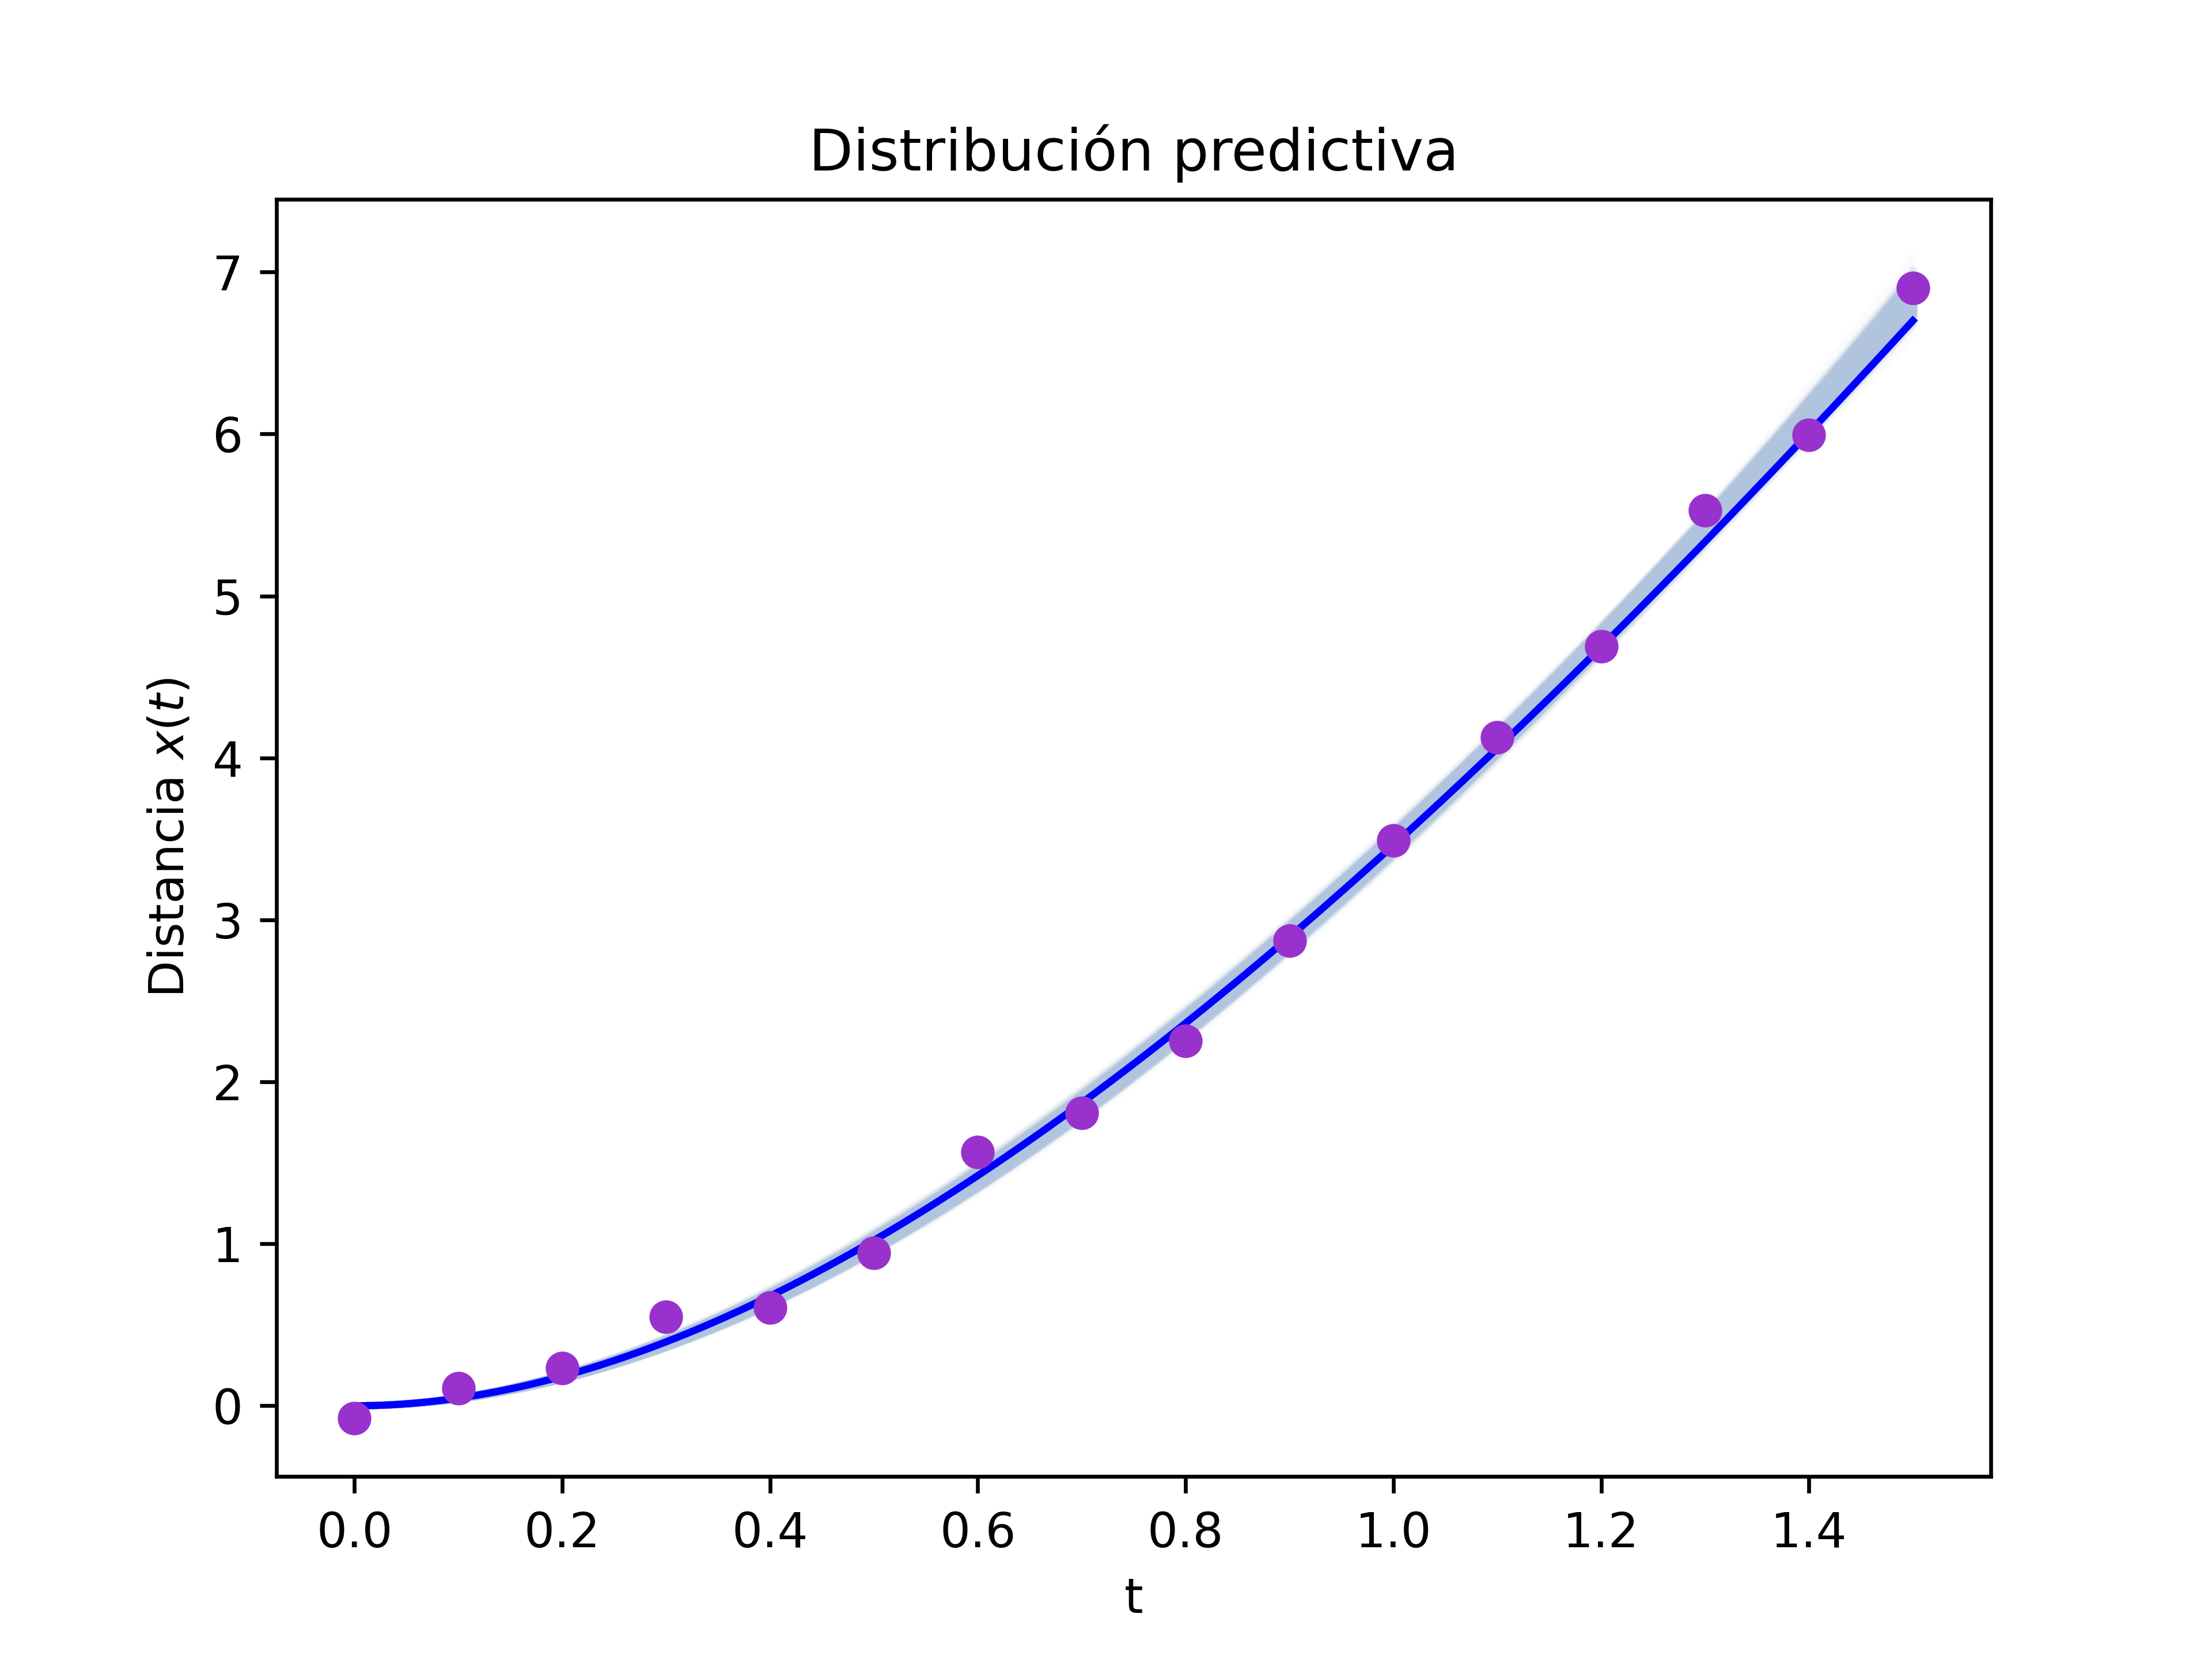
\includegraphics[width = 10 cm ]{img/Exp_Central_gravedad_sigma/Figuras/Generales/Predictiva_gravedad_sigma.png} 
    % \caption{Distribución predictiva para el modelo gravitatorio}
    \label{Fig. 3.2.2.06}
  \end{figure} 
\end{frame}

\begin{frame}{Simulación del Modelo Gravitatorio}
  \begin{figure}[H]
    \centering 
    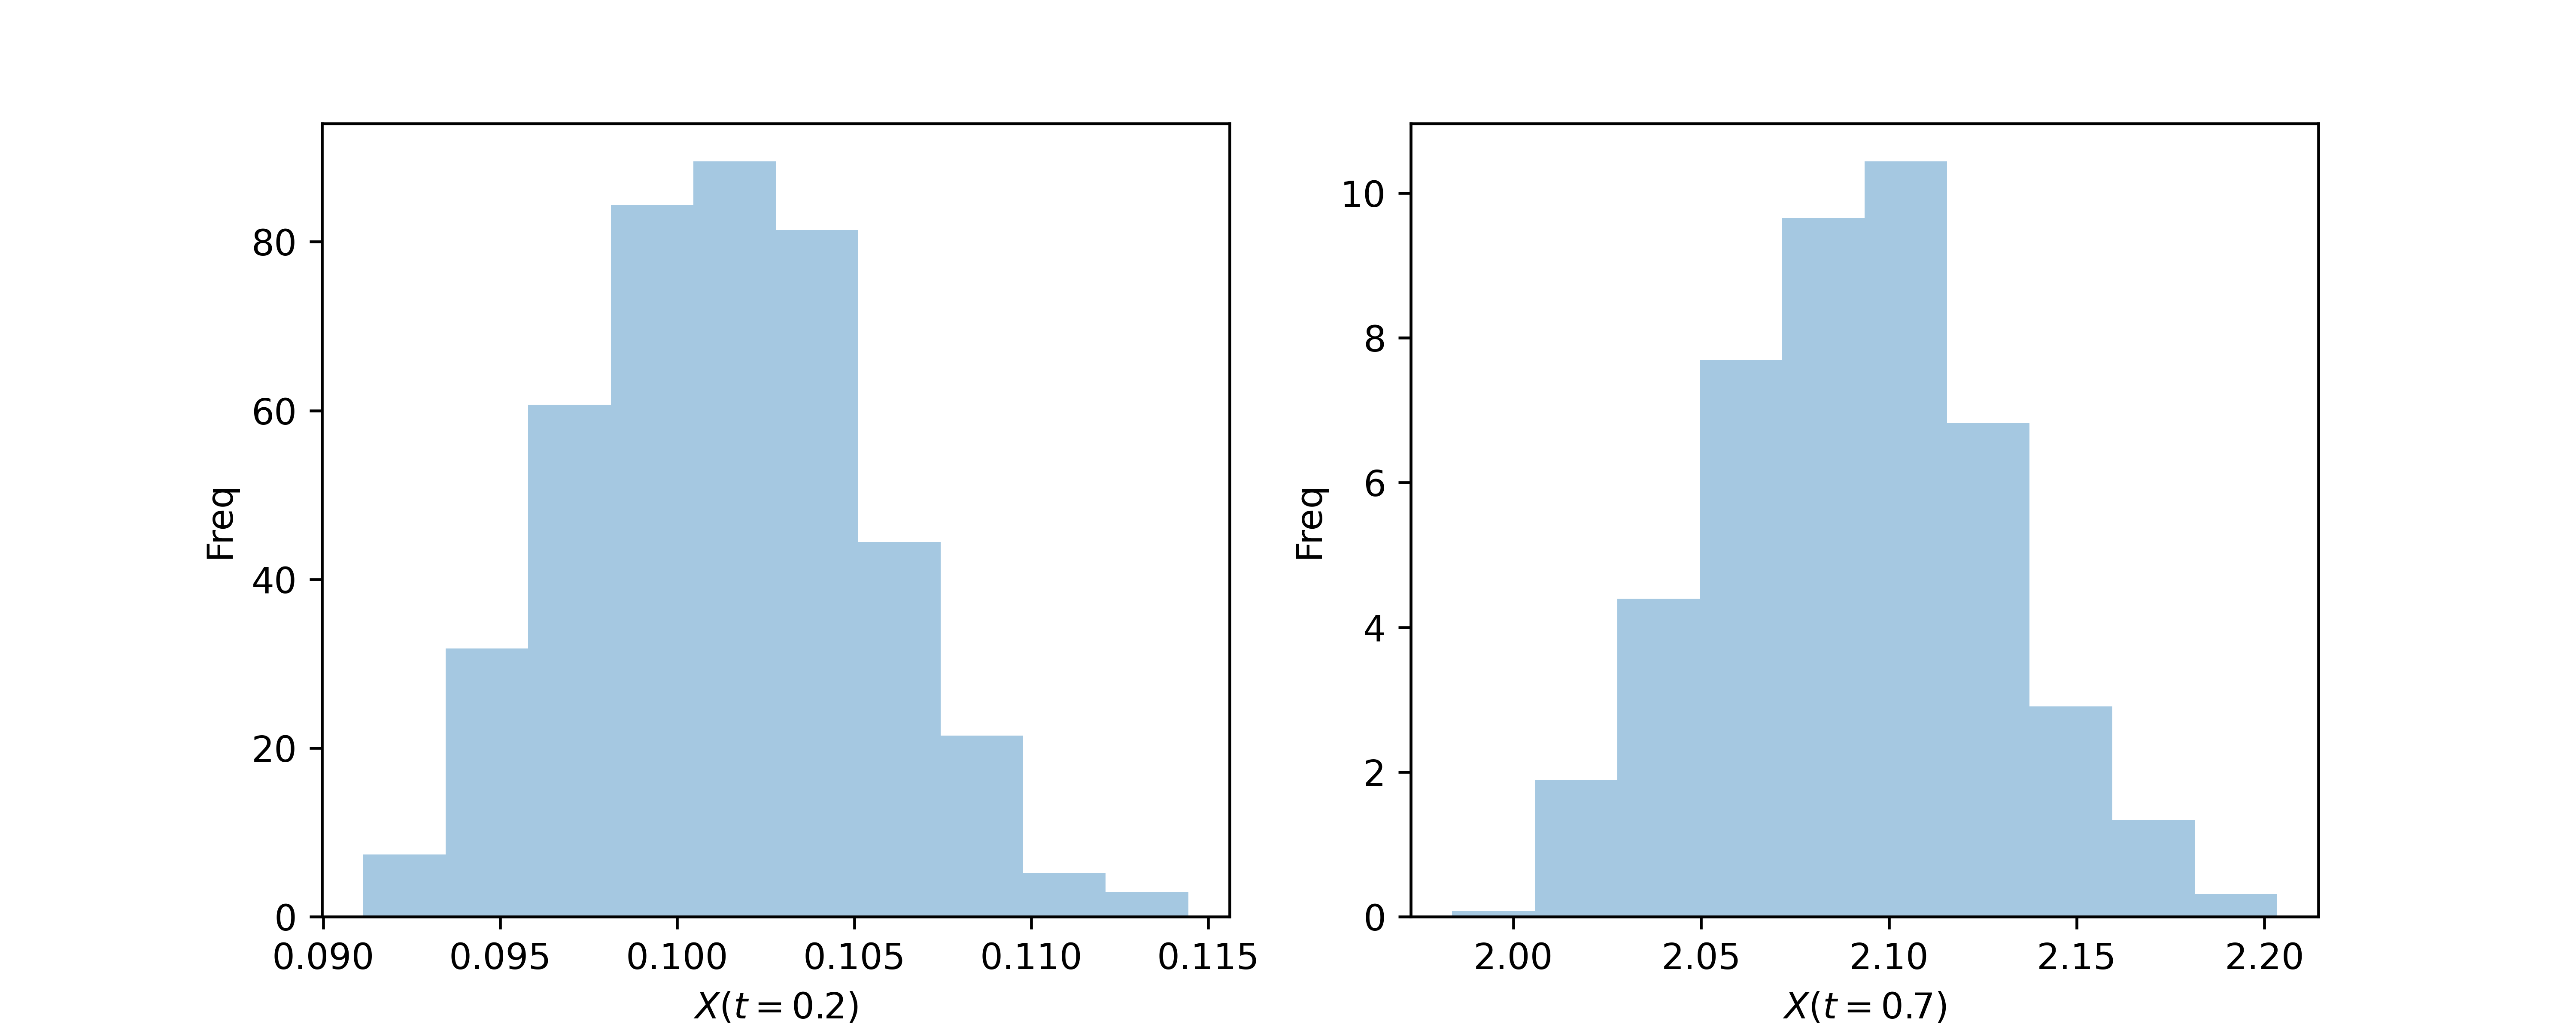
\includegraphics[width = 13 cm]{img/Exp_Central_gravedad_sigma/Figuras/Generales/TiempoFijo_gravedad_sigma.png} 
    % \caption{Distribución predictiva del modelo gravitatorio para los valores de tiempo de 0.2s y 0.7s.}
    \label{Fig. 3.2.2.07}
  \end{figure}
\end{frame}


% \begin{frame}{Simulación del Modelo Logístico}
%   \begin{figure}
%     \centering 
%     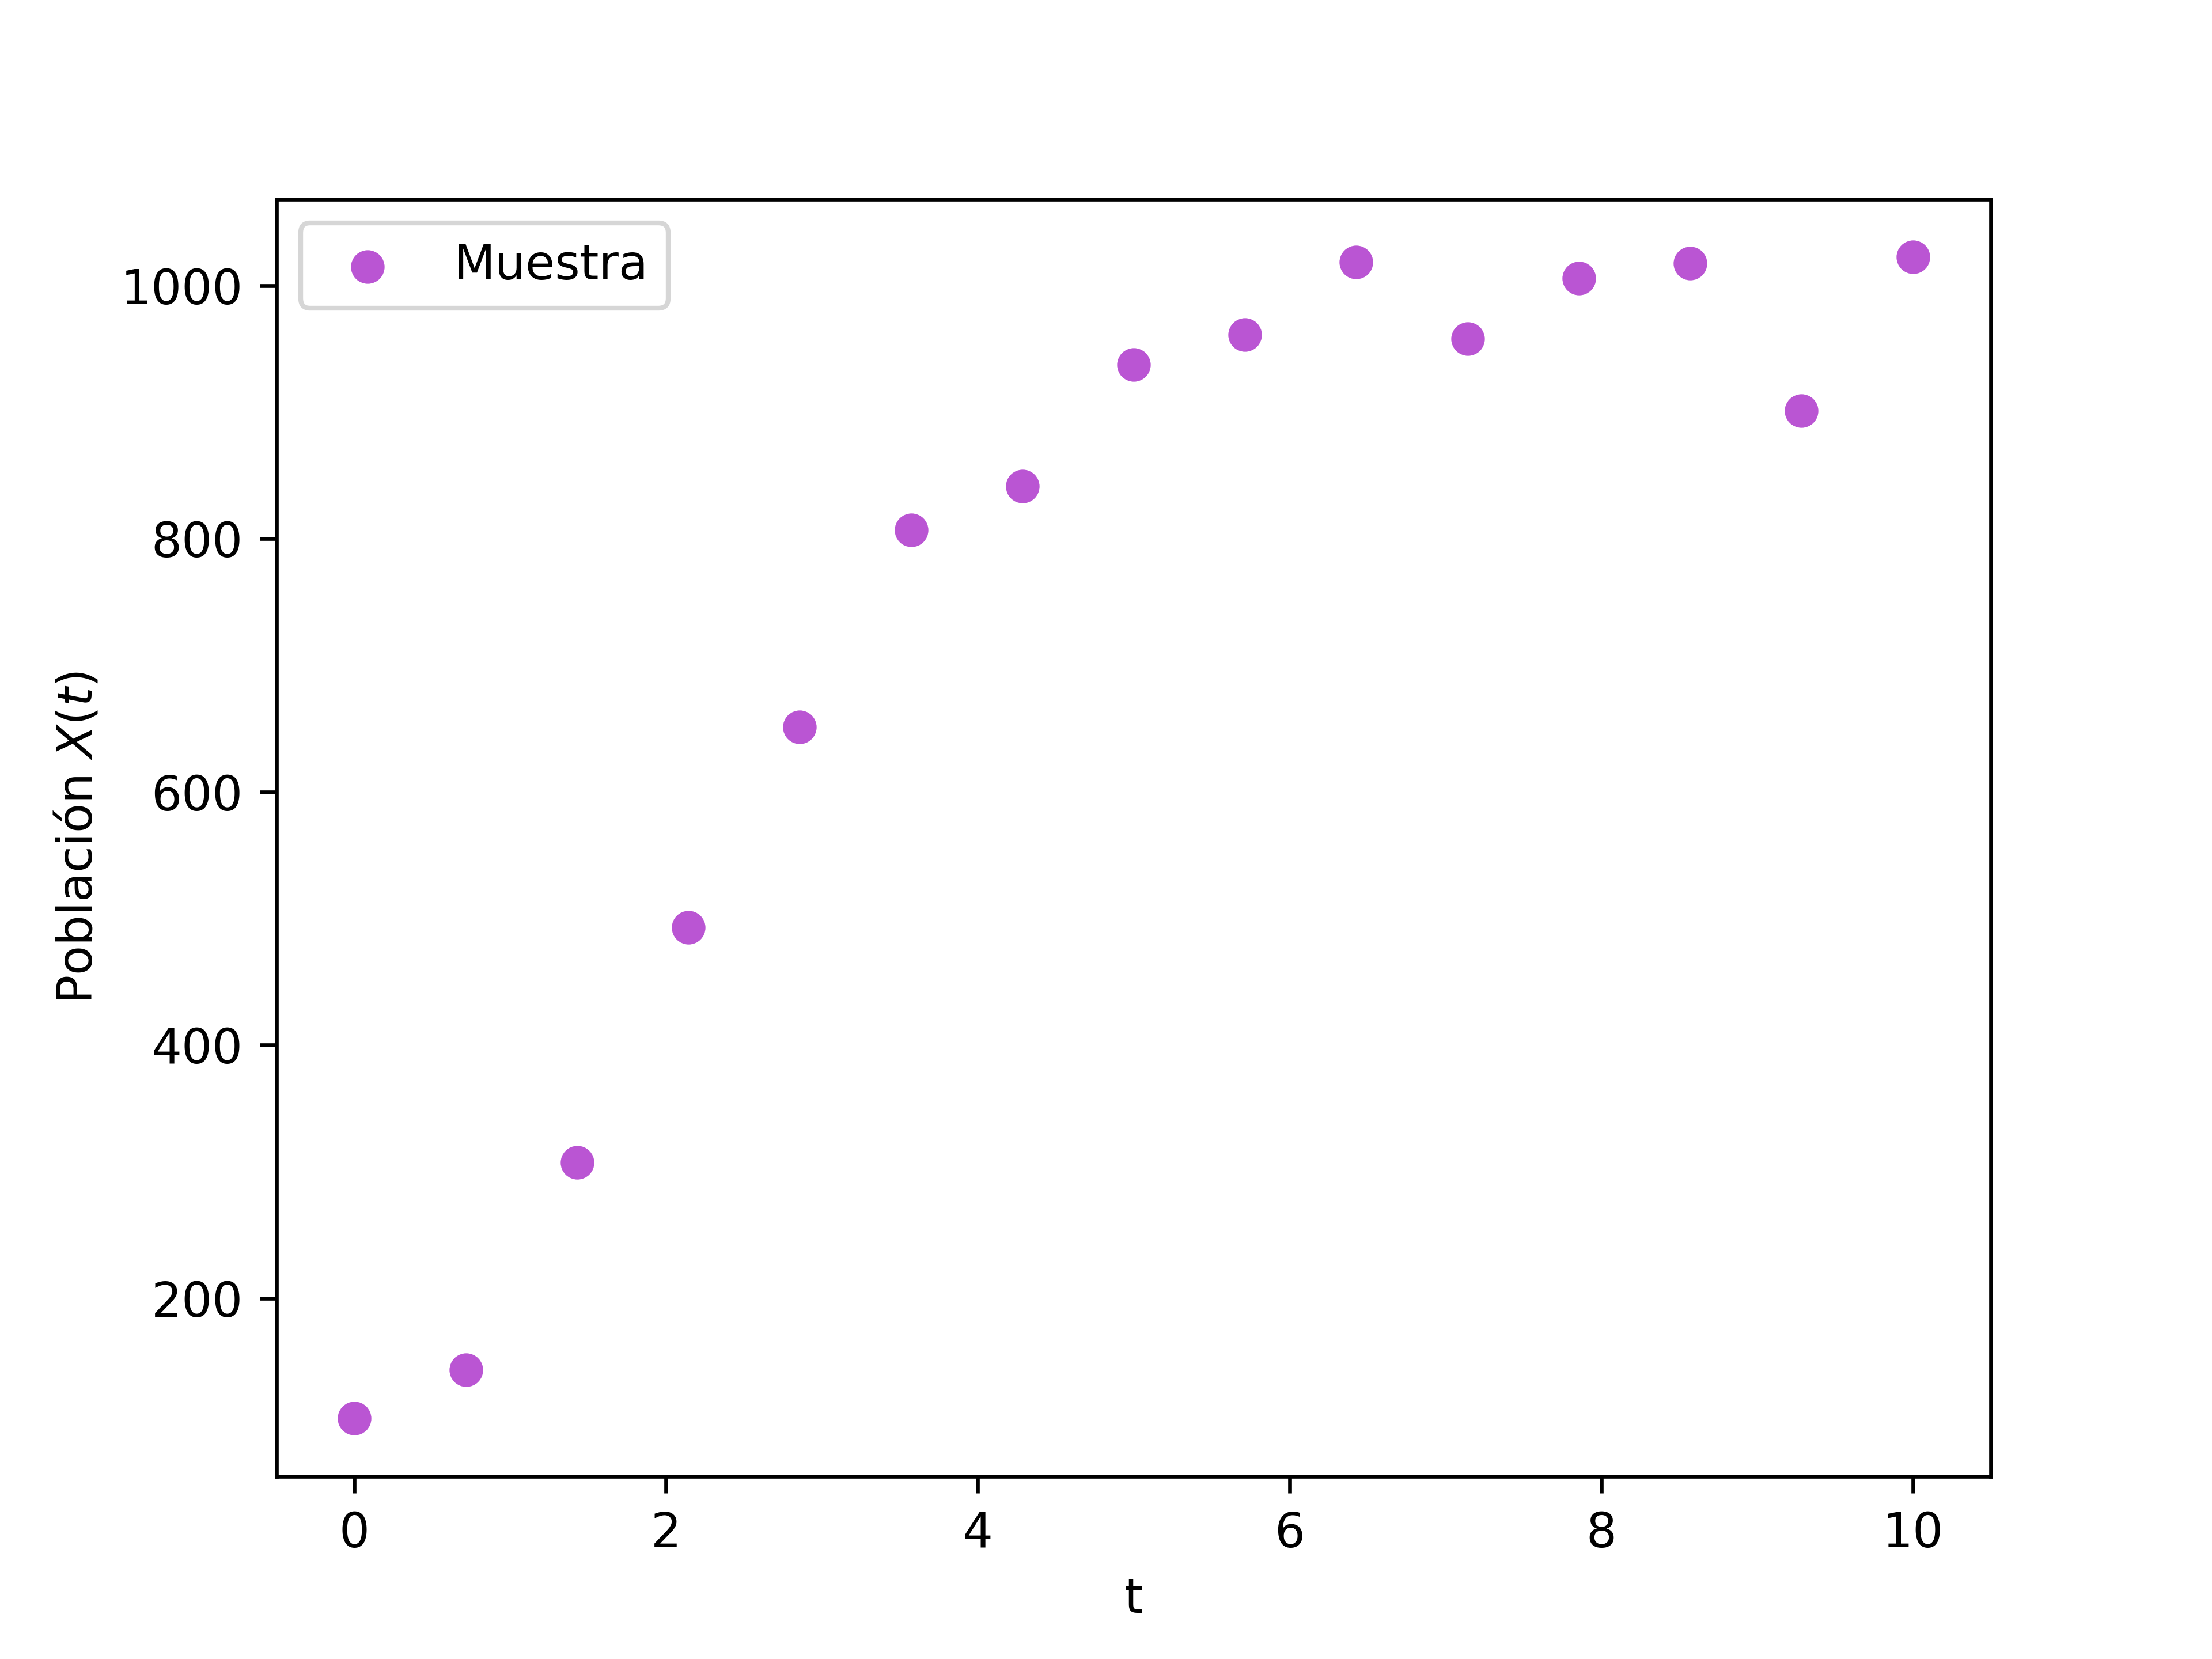
\includegraphics[width = 9 cm ]{img/Exp_Central_logistico_sigma/Figuras/Generales/Muestra_logistico_sigma.png} 
%     % \caption{Muestra $\mathbf{y}$ para el modelo logístico.}
%     \label{Fig. 3.2.log.muestra}
%   \end{figure} 
% \end{frame}


% \begin{frame}{Simulación del Modelo Logístico}
%   \begin{figure} 
%     \centering 
%     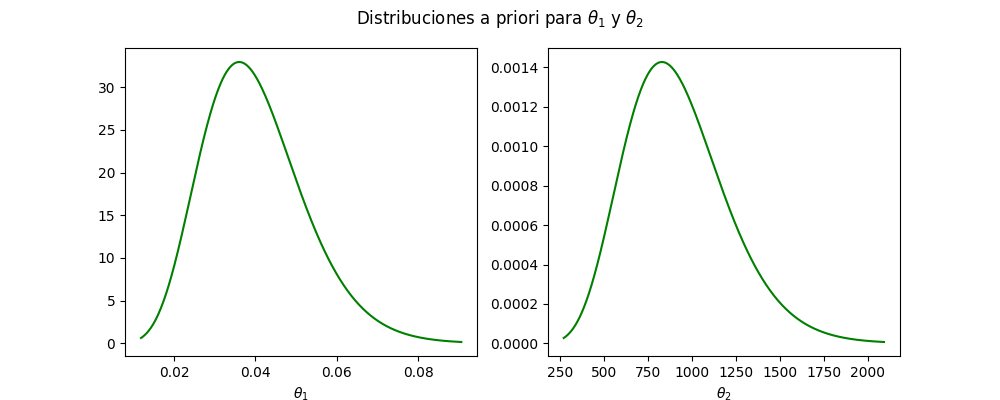
\includegraphics[width = 15 cm]{img/Exp_Central_logistico_sigma/Figuras/Generales/Apriori_logistico_sigma.png}     
%     % \caption{Distribuciones a priori para $\theta_1$ y $\theta_2$}
%     \label{Fig. 3.2.log.priori}
%   \end{figure} 
% \end{frame}


% \begin{frame}{Simulación del Modelo Logístico}
%   \begin{figure}
%     \centering 
%     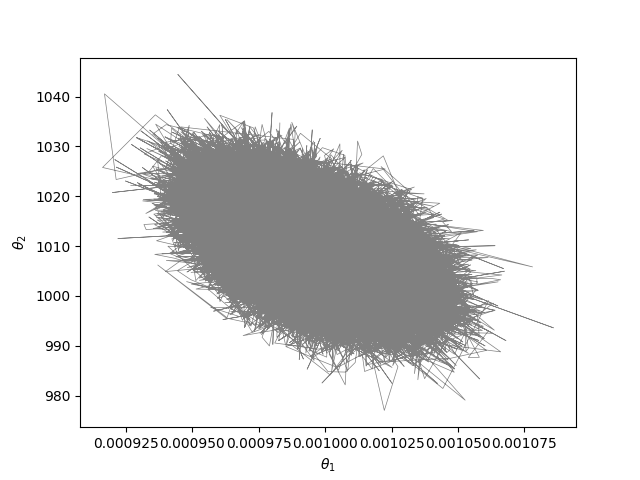
\includegraphics[width = 10 cm ]{img/Exp_Central_logistico_sigma/Figuras/Generales/Conjunta_logistico_sigma.png} 
%     \caption{Posterior conjunta para el modelo logístico.}
%     \label{Fig. 3.2.log.conjunta}
%   \end{figure} 
% \end{frame}


% \begin{frame}{Simulación del Modelo Logístico}
%   \begin{columns}[T,onlytextwidth]
%     \column{0.5\textwidth}
    
%     \begin{figure}
%       \centering 
%       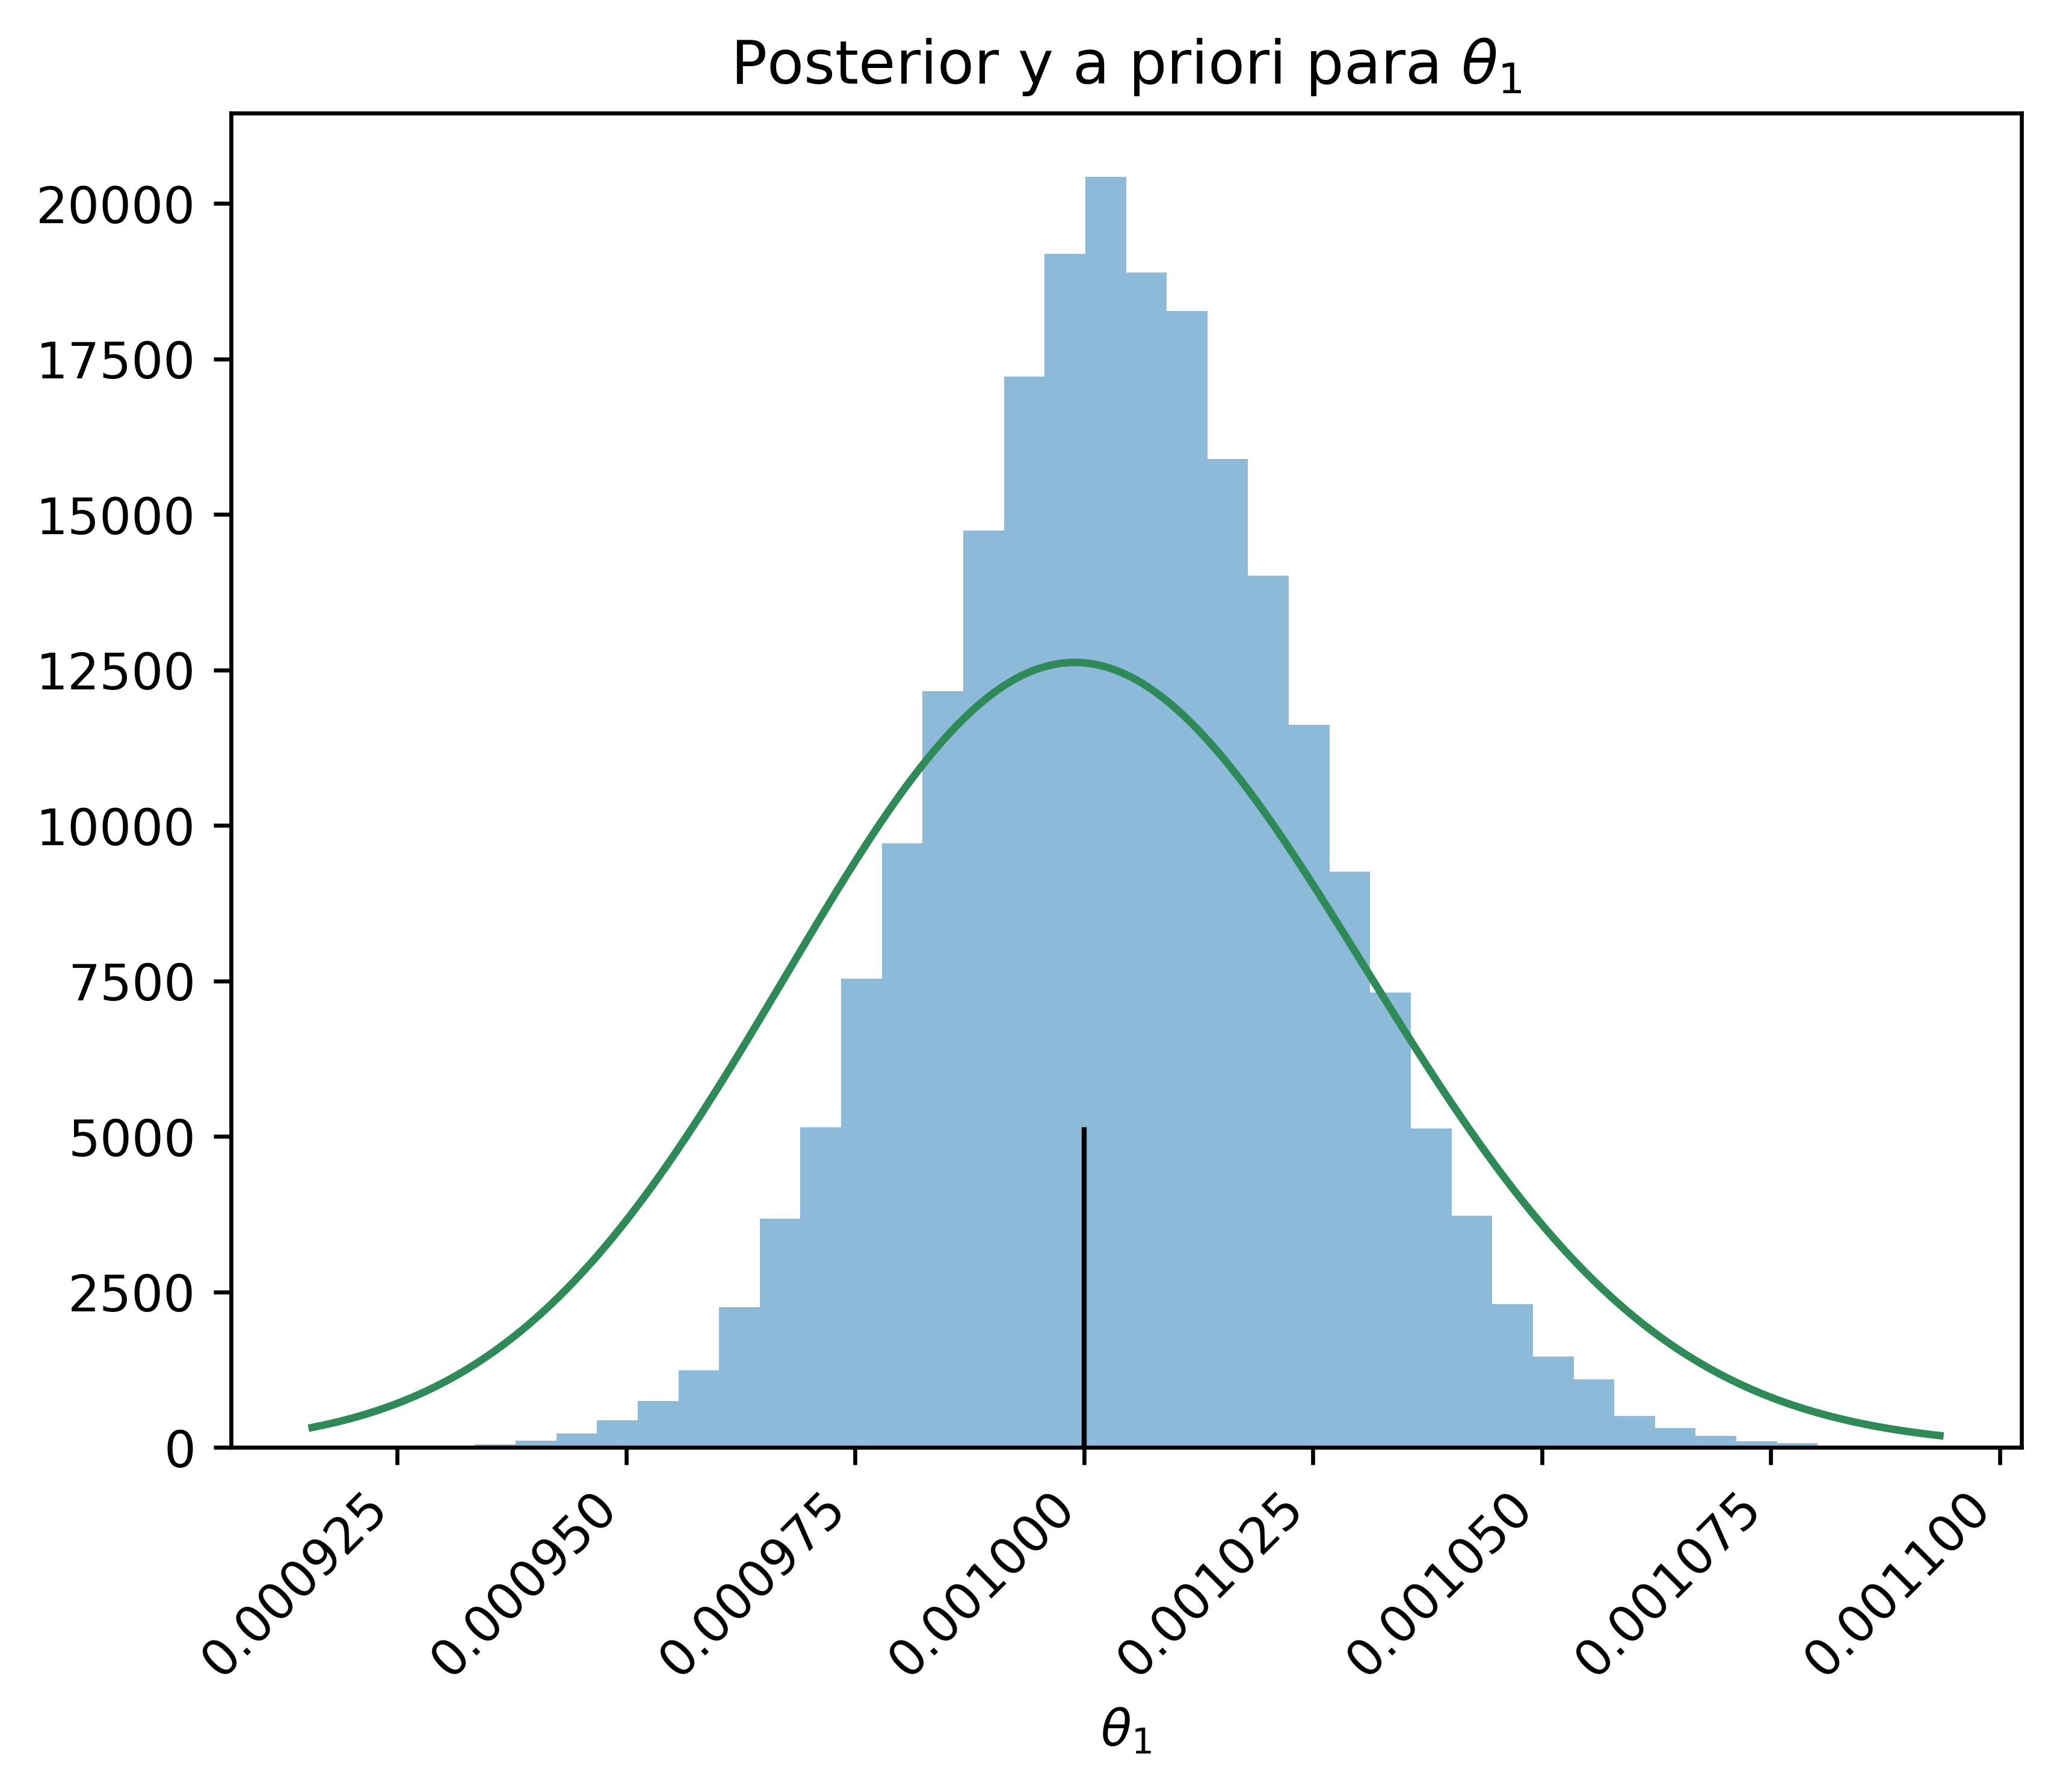
\includegraphics[width=0.9\textwidth]{img/Exp_Central_logistico_sigma/Figuras/Generales/Post_theta1_logistico_sigma.png}
%     \end{figure} 
    
%     \column{0.5\textwidth}
    
%       % \metroset{block=fill}
      
%     \begin{figure}
%       \centering 
%       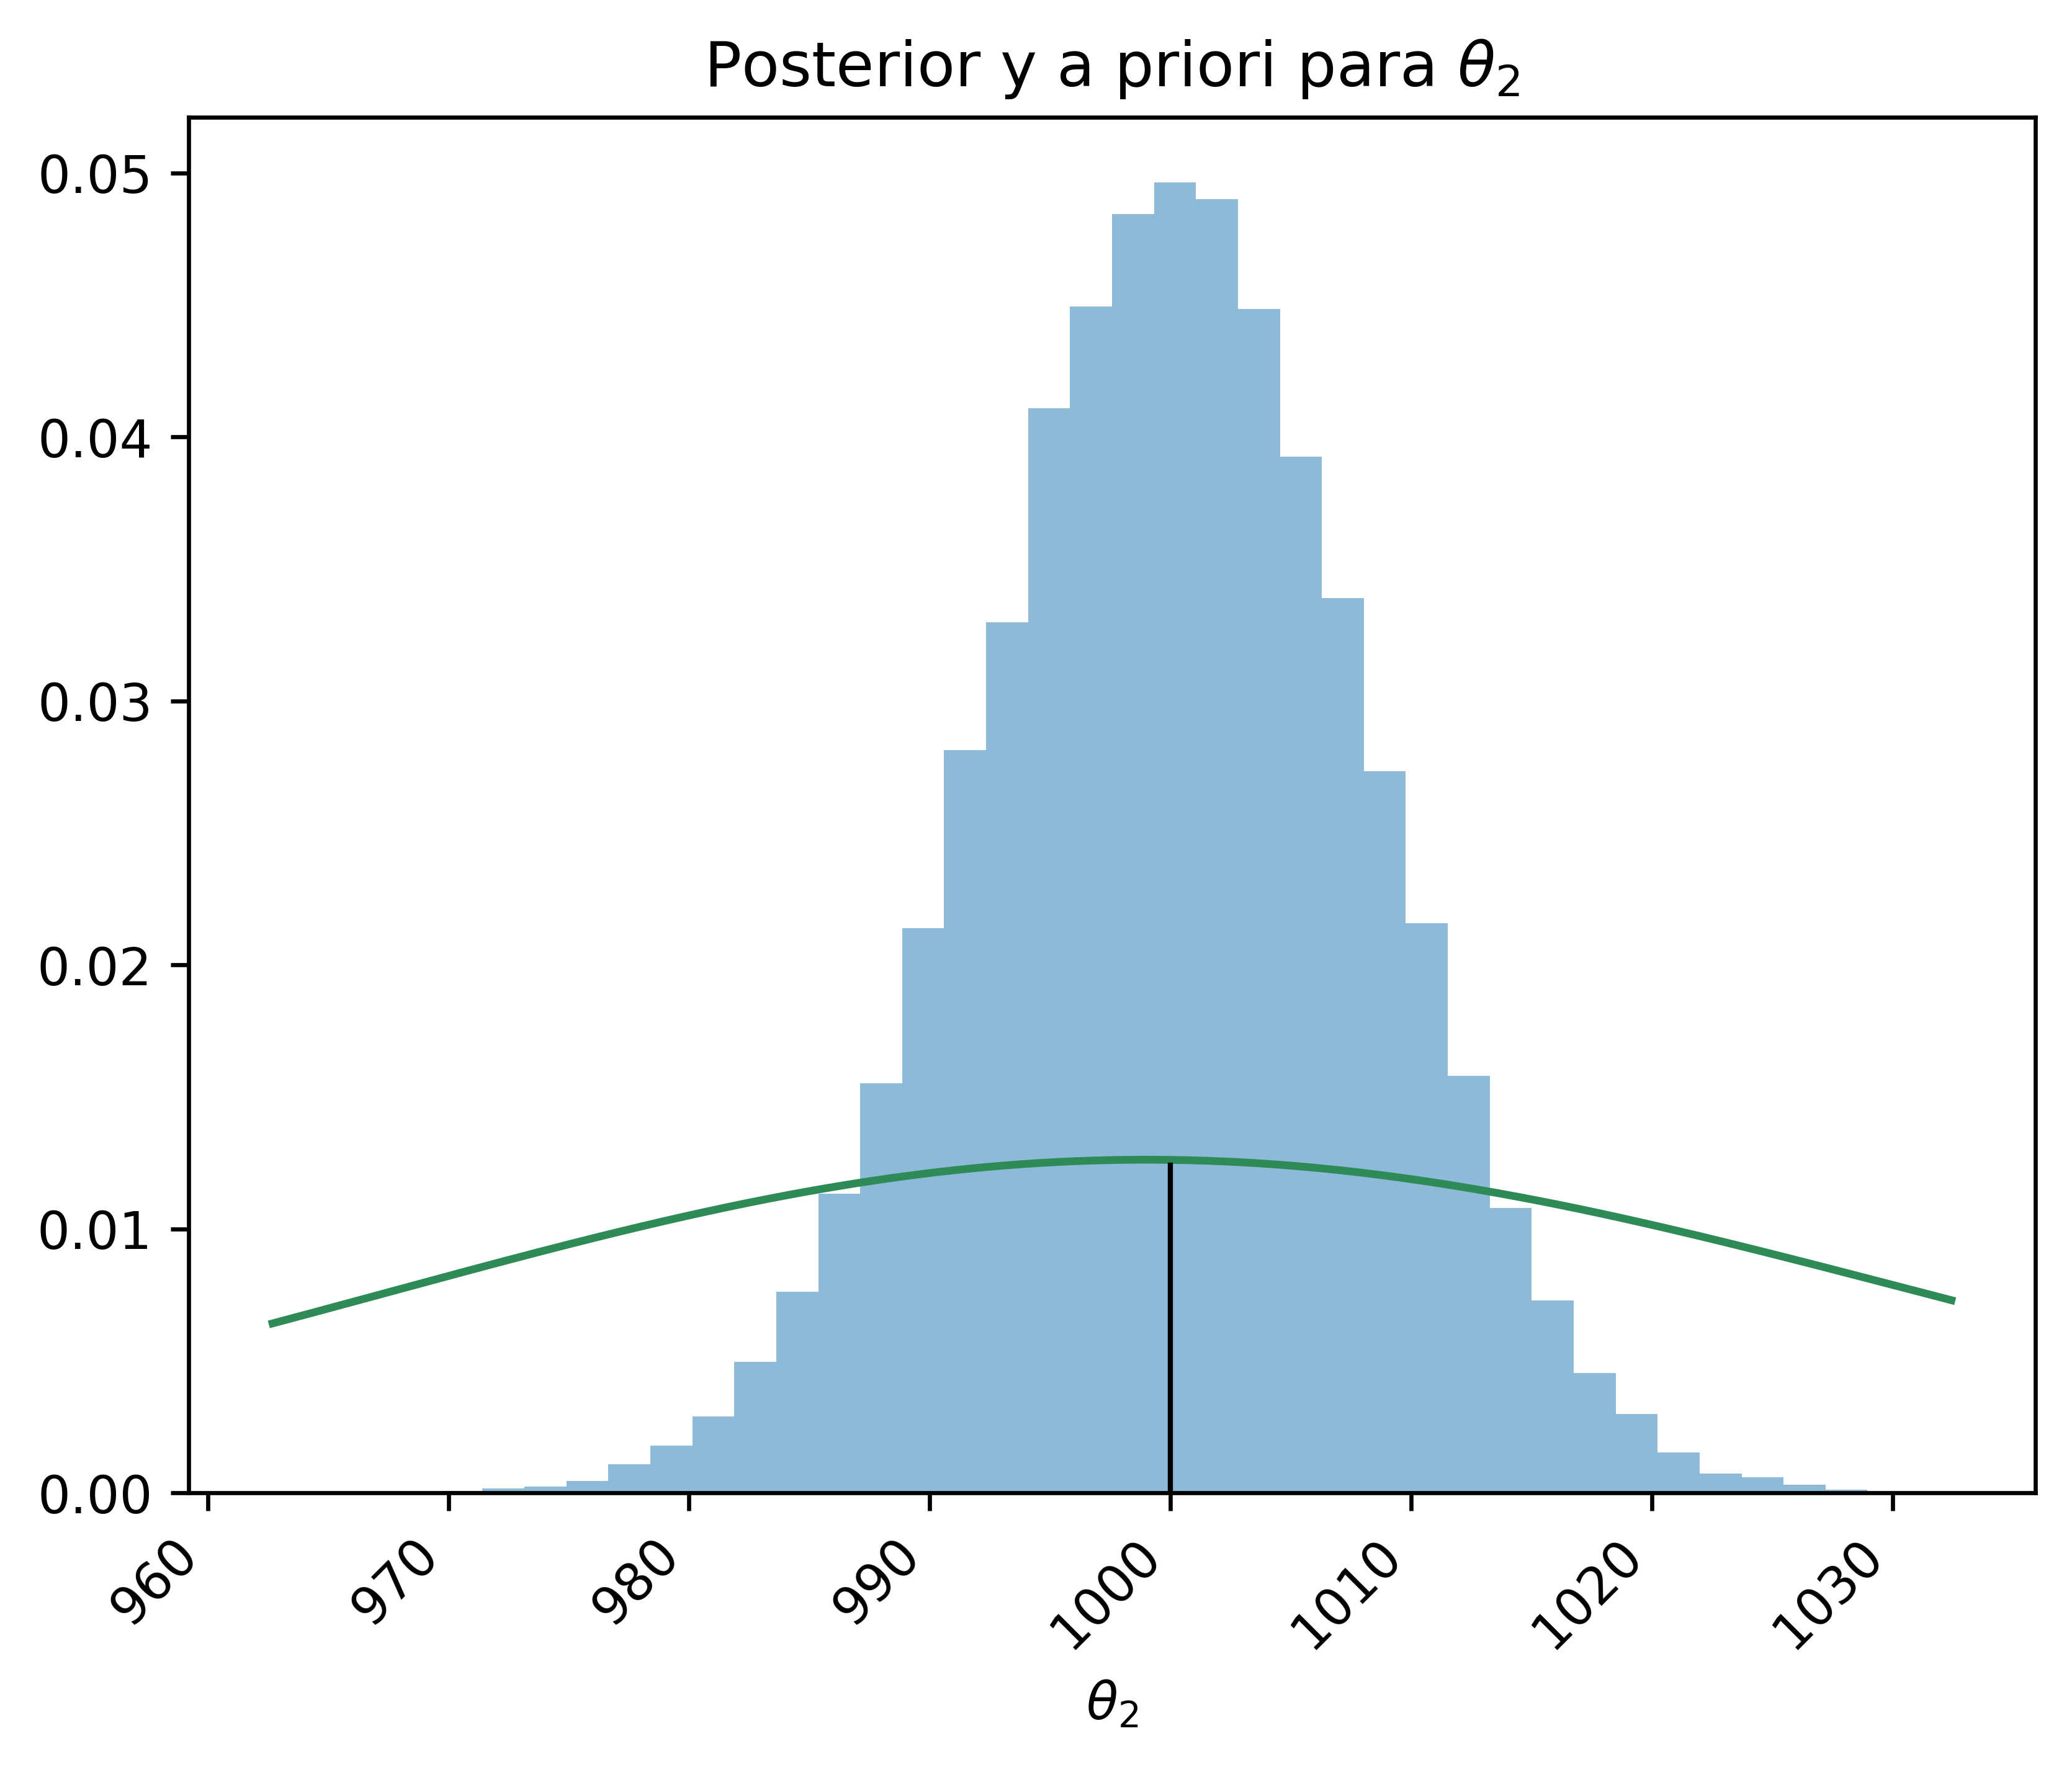
\includegraphics[width=0.9\textwidth]{img/Exp_Central_logistico_sigma/Figuras/Generales/Post_theta2_logistico_sigma.png}
%     \end{figure} 
    
%   \end{columns}
% \end{frame}


% \begin{frame}{Simulación del Modelo Logístico}
%   \begin{figure}
%     \centering 
%     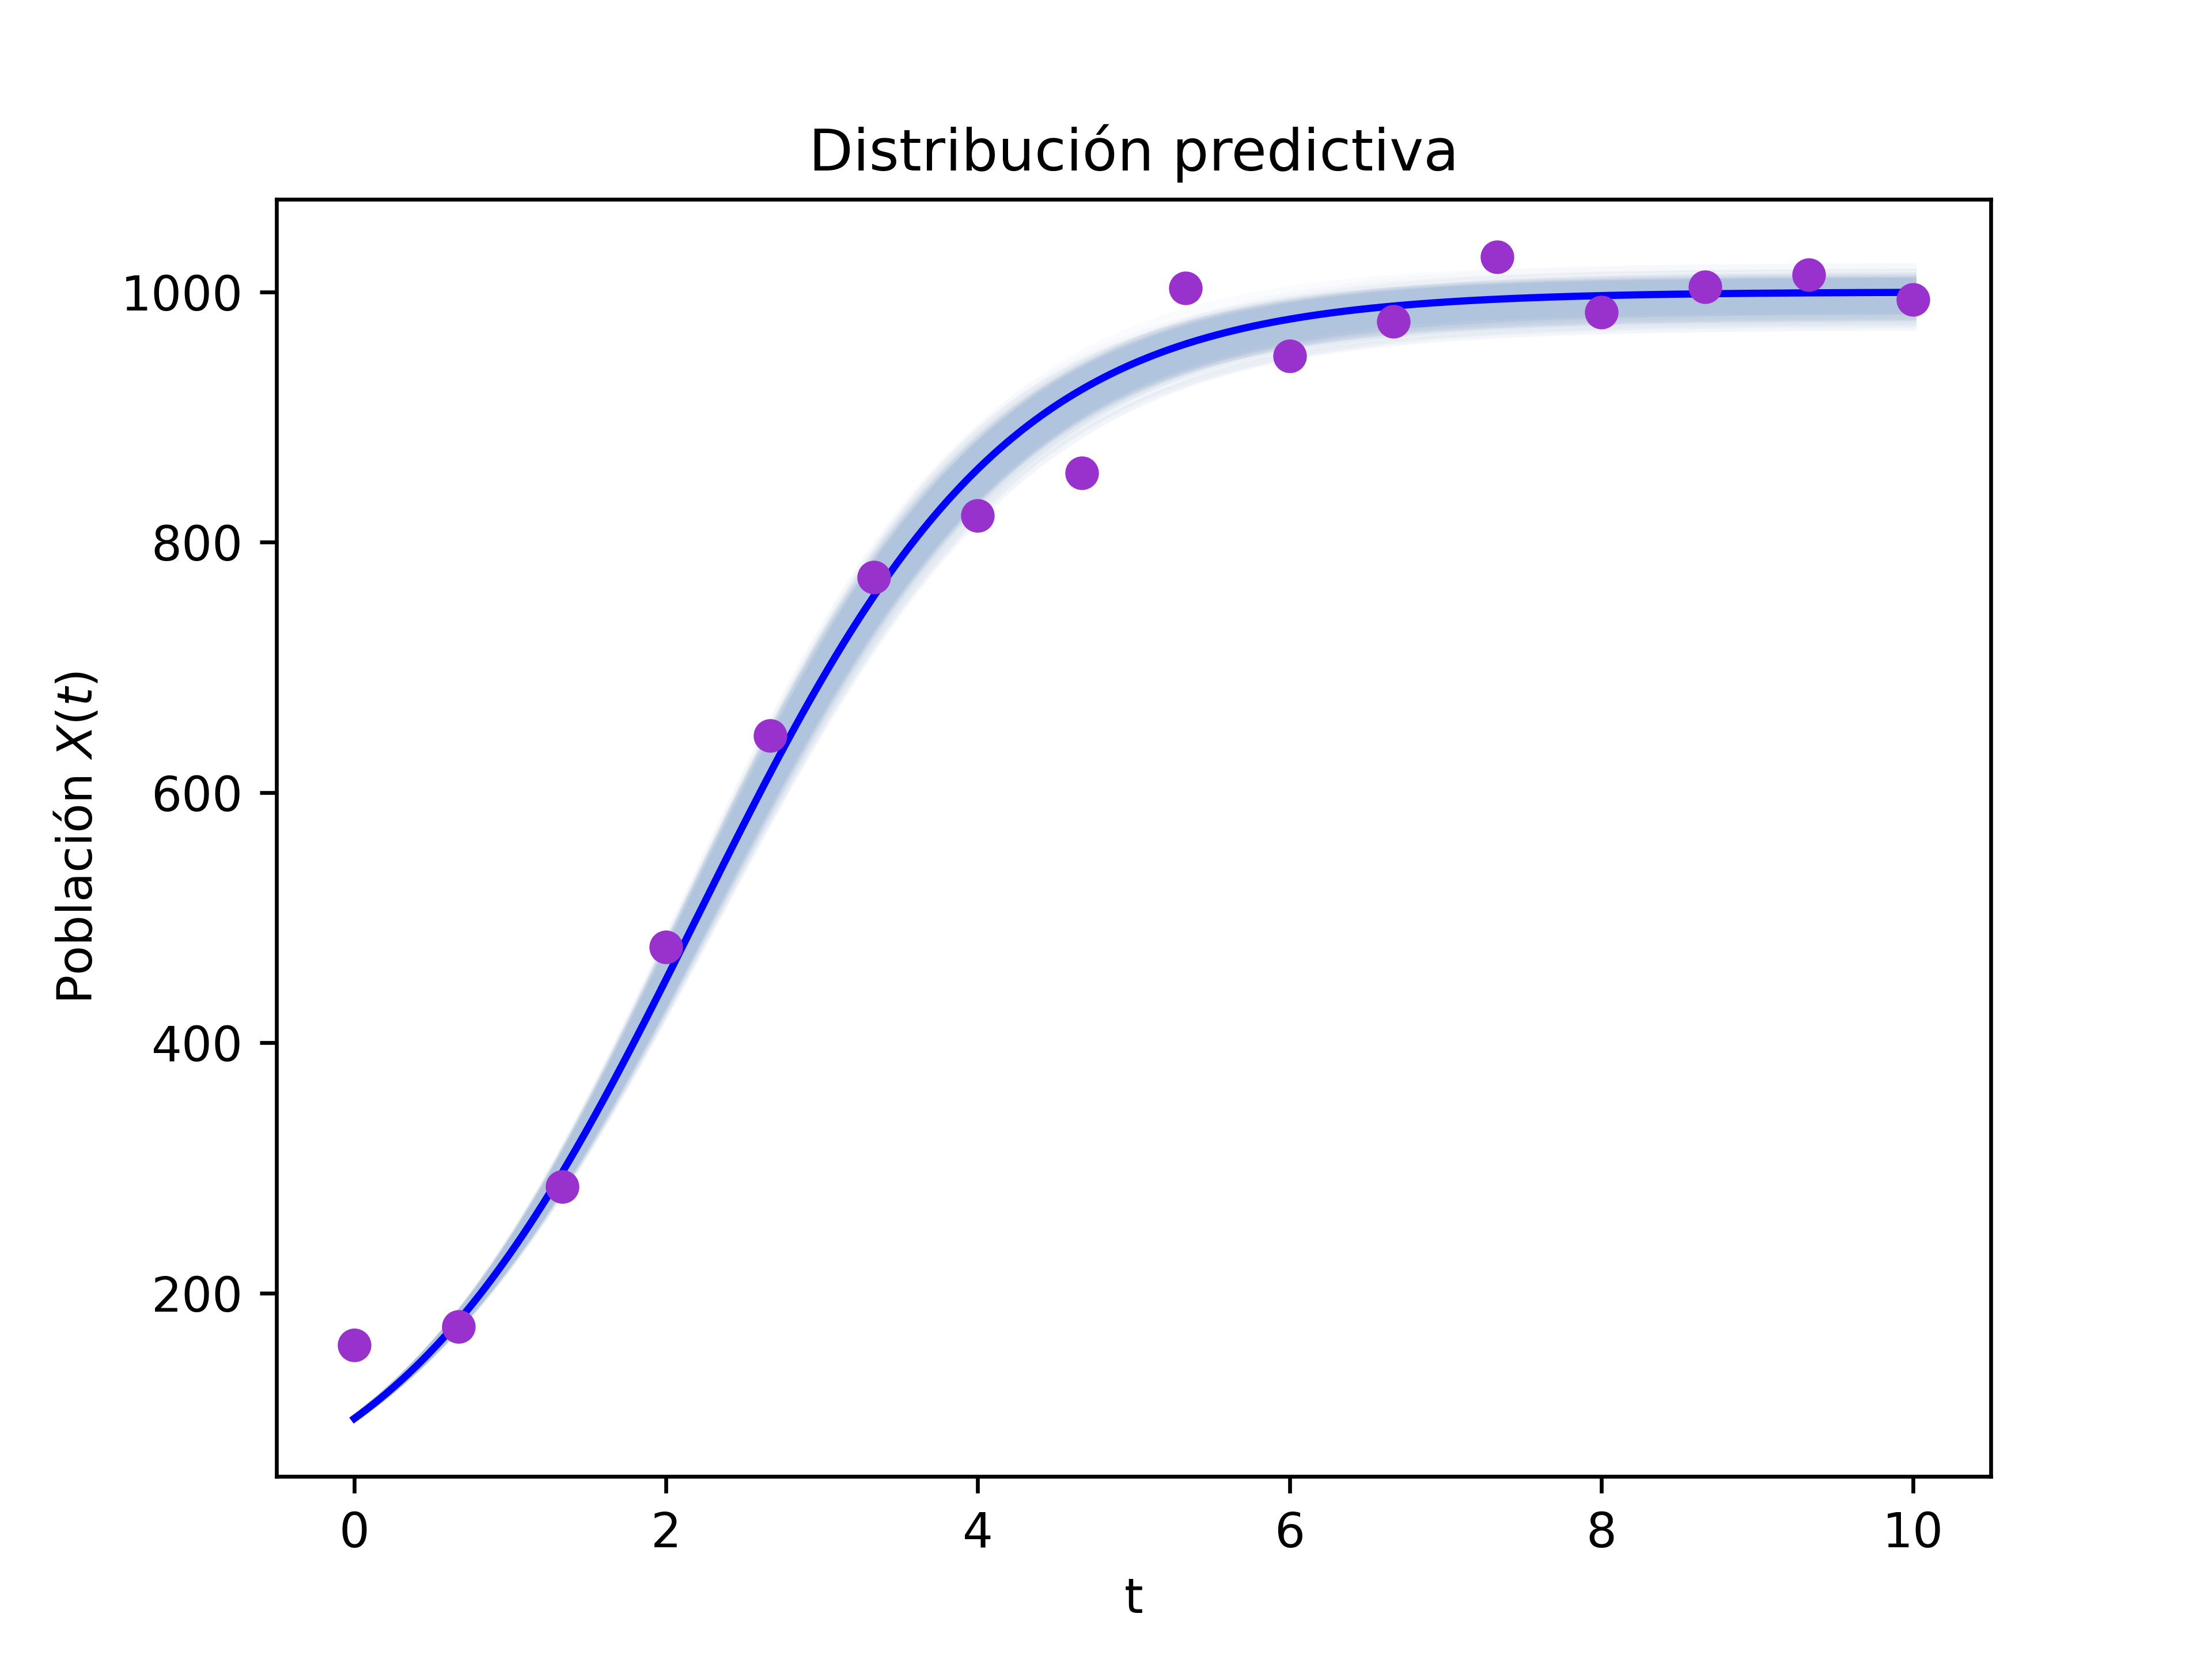
\includegraphics[width = 10 cm ]{img/Exp_Central_logistico_sigma/Figuras/Generales/Predictiva_logistico_sigma.png} 
%     % \caption{Distribución predictiva para el modelo logístico.}
%     \label{Fig. 3.2.log.predictiva}
%   \end{figure} 
% \end{frame}


% \begin{frame}{Simulación del Modelo SIR}
%   \begin{figure}
%     \centering 
%     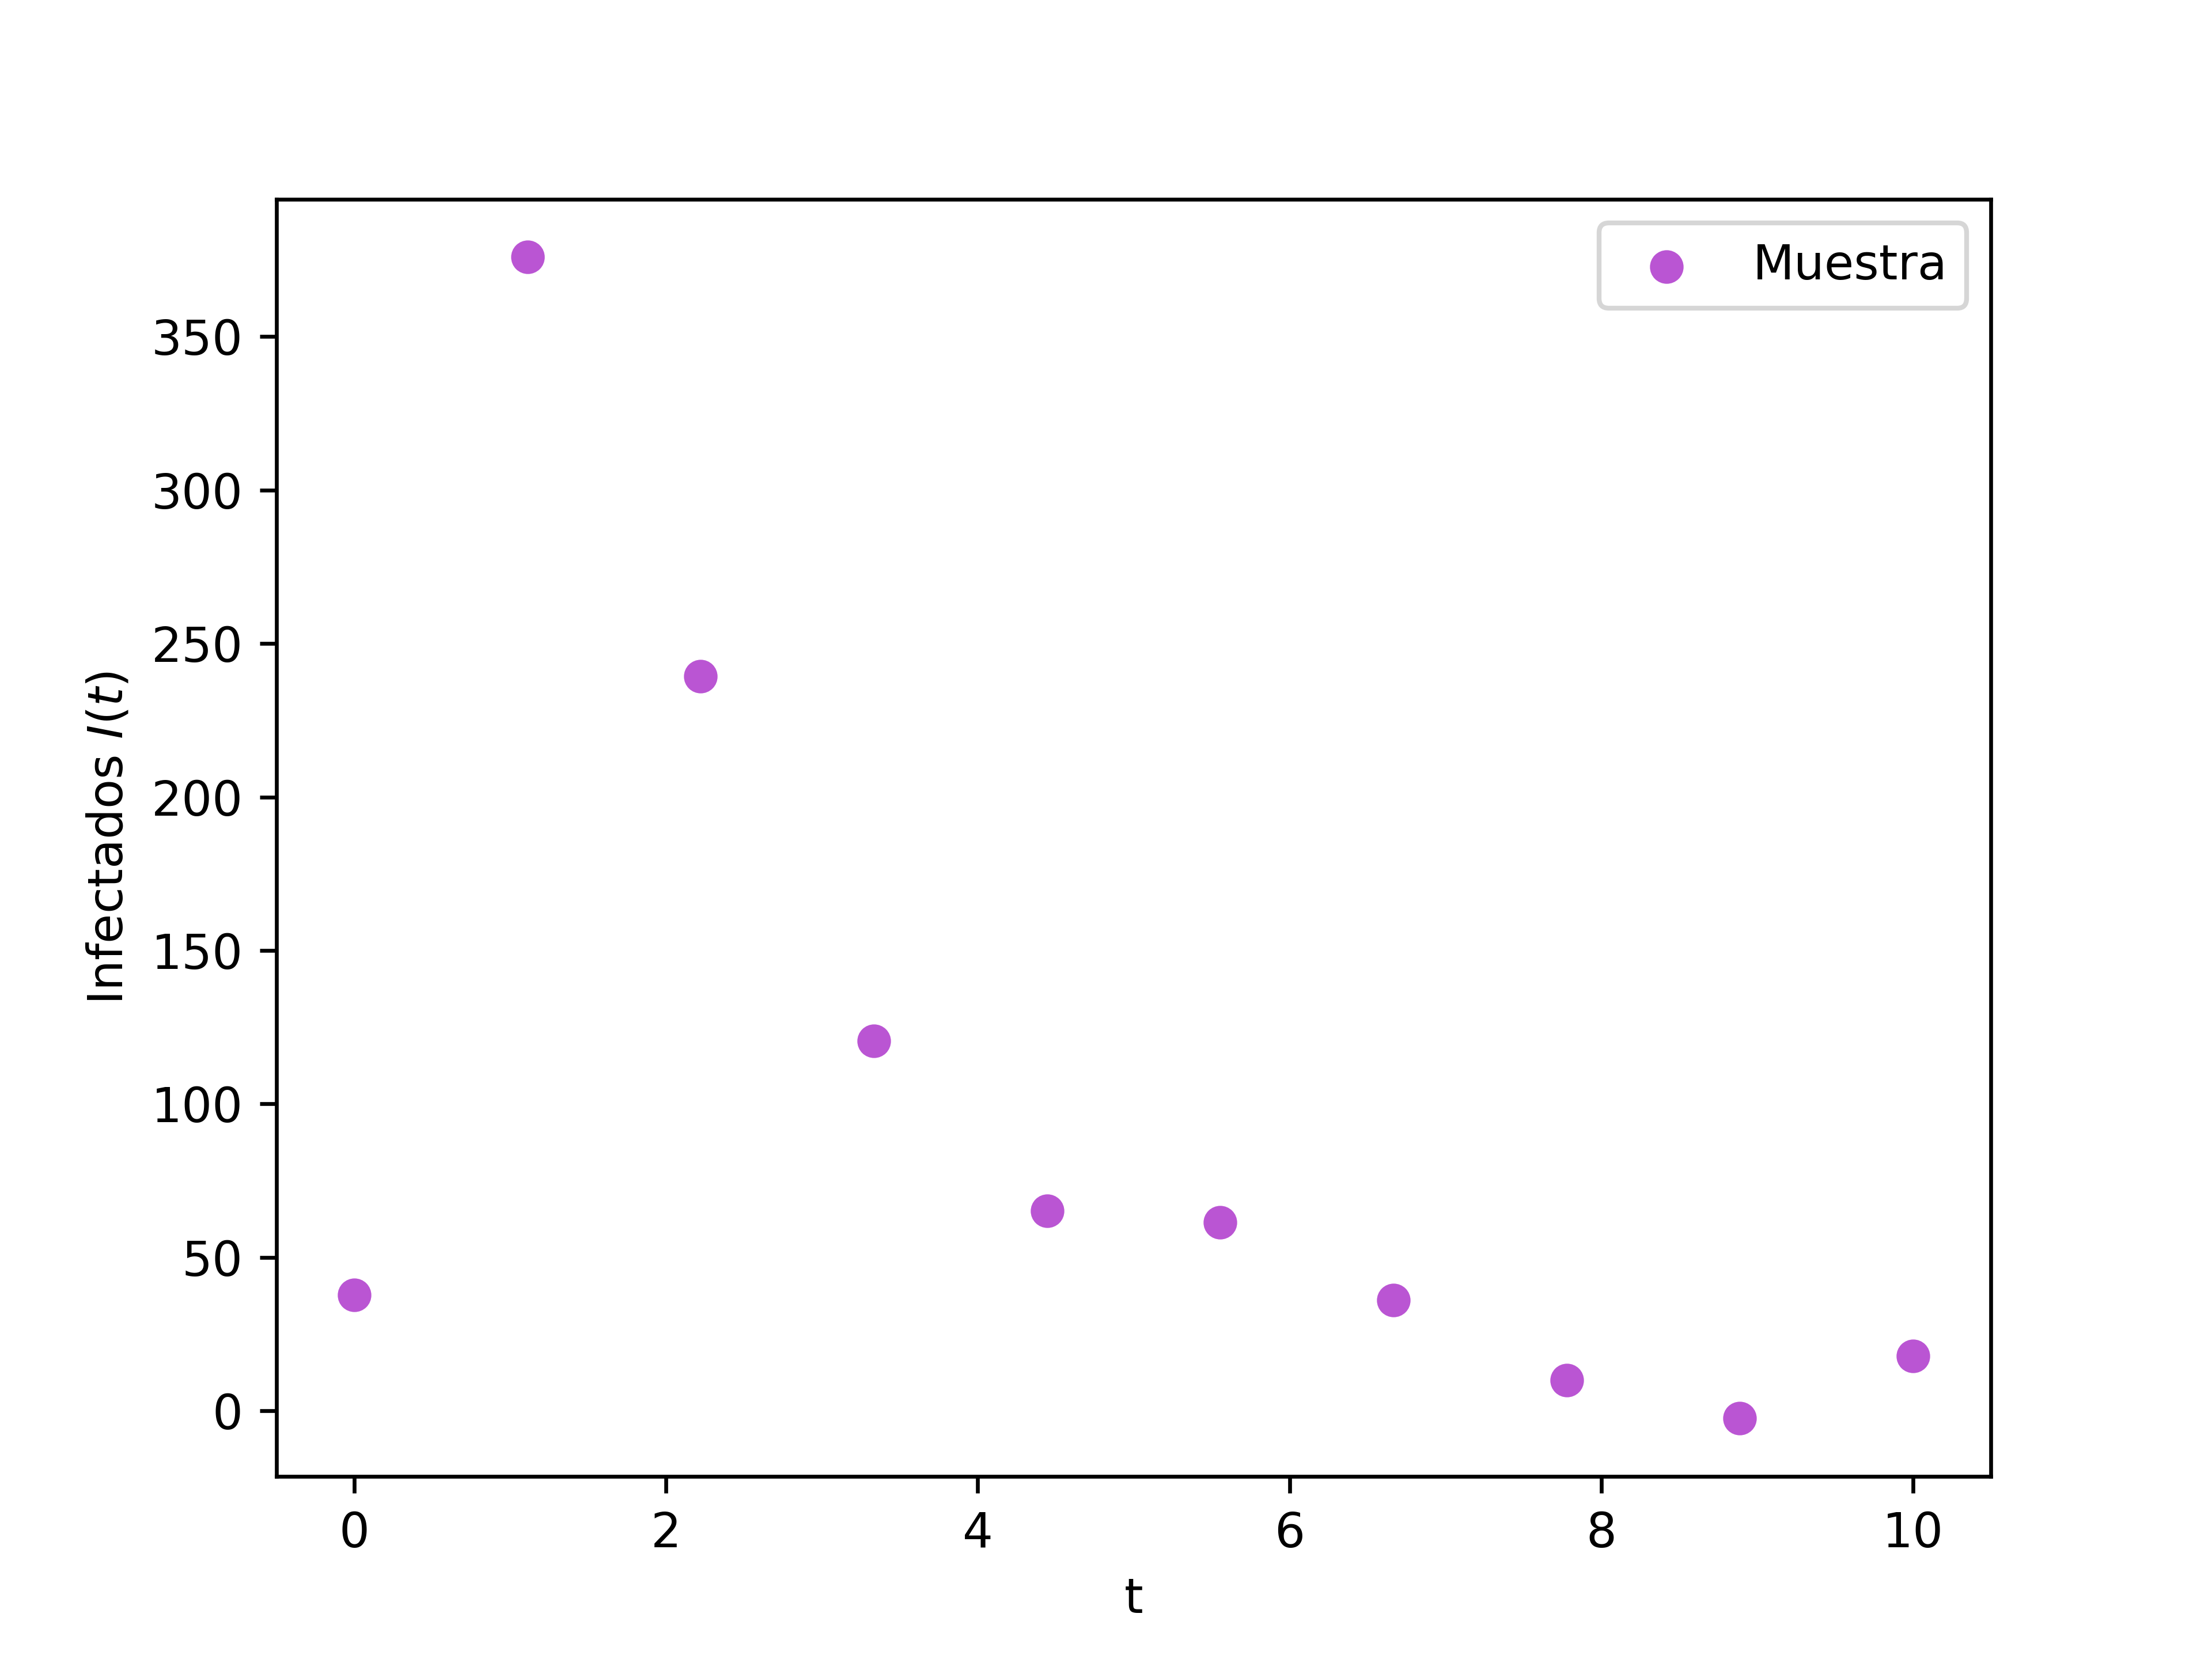
\includegraphics[width = 10 cm]{img/Exp_Central_SIR_sigma/Figuras/Generales/Muestra_SIR_sigma.png} 
%     % \caption{Muestra $\mathbf{y}$ del modelo SIR.}
%     \label{Fig. SIR_01}
%   \end{figure} 
% \end{frame}

% \begin{frame}{Simulación del Modelo SIR}
%   \begin{figure}[H] 
%     \centering 
%     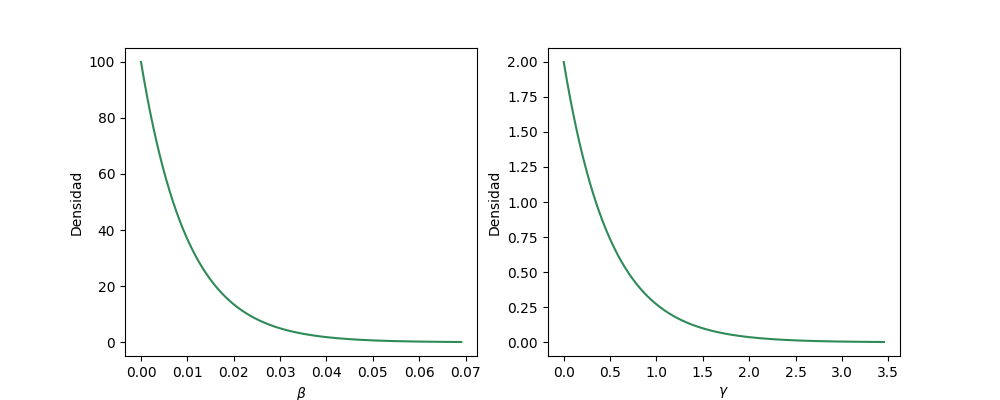
\includegraphics[width = 12 cm ]{img/Exp_Central_SIR_sigma/Figuras/Generales/Apriori_SIR_sigma.png} 
%     % \caption{Distribuciones marginal a priori para el parámetro $\beta$ (izquierda) y $\gamma$ (derecha).}
%     \label{Fig. SIR_02}
%   \end{figure} 
% \end{frame}



% \begin{frame}{Simulación del Modelo SIR}
%   \begin{figure}[H] 
%     \centering 
%     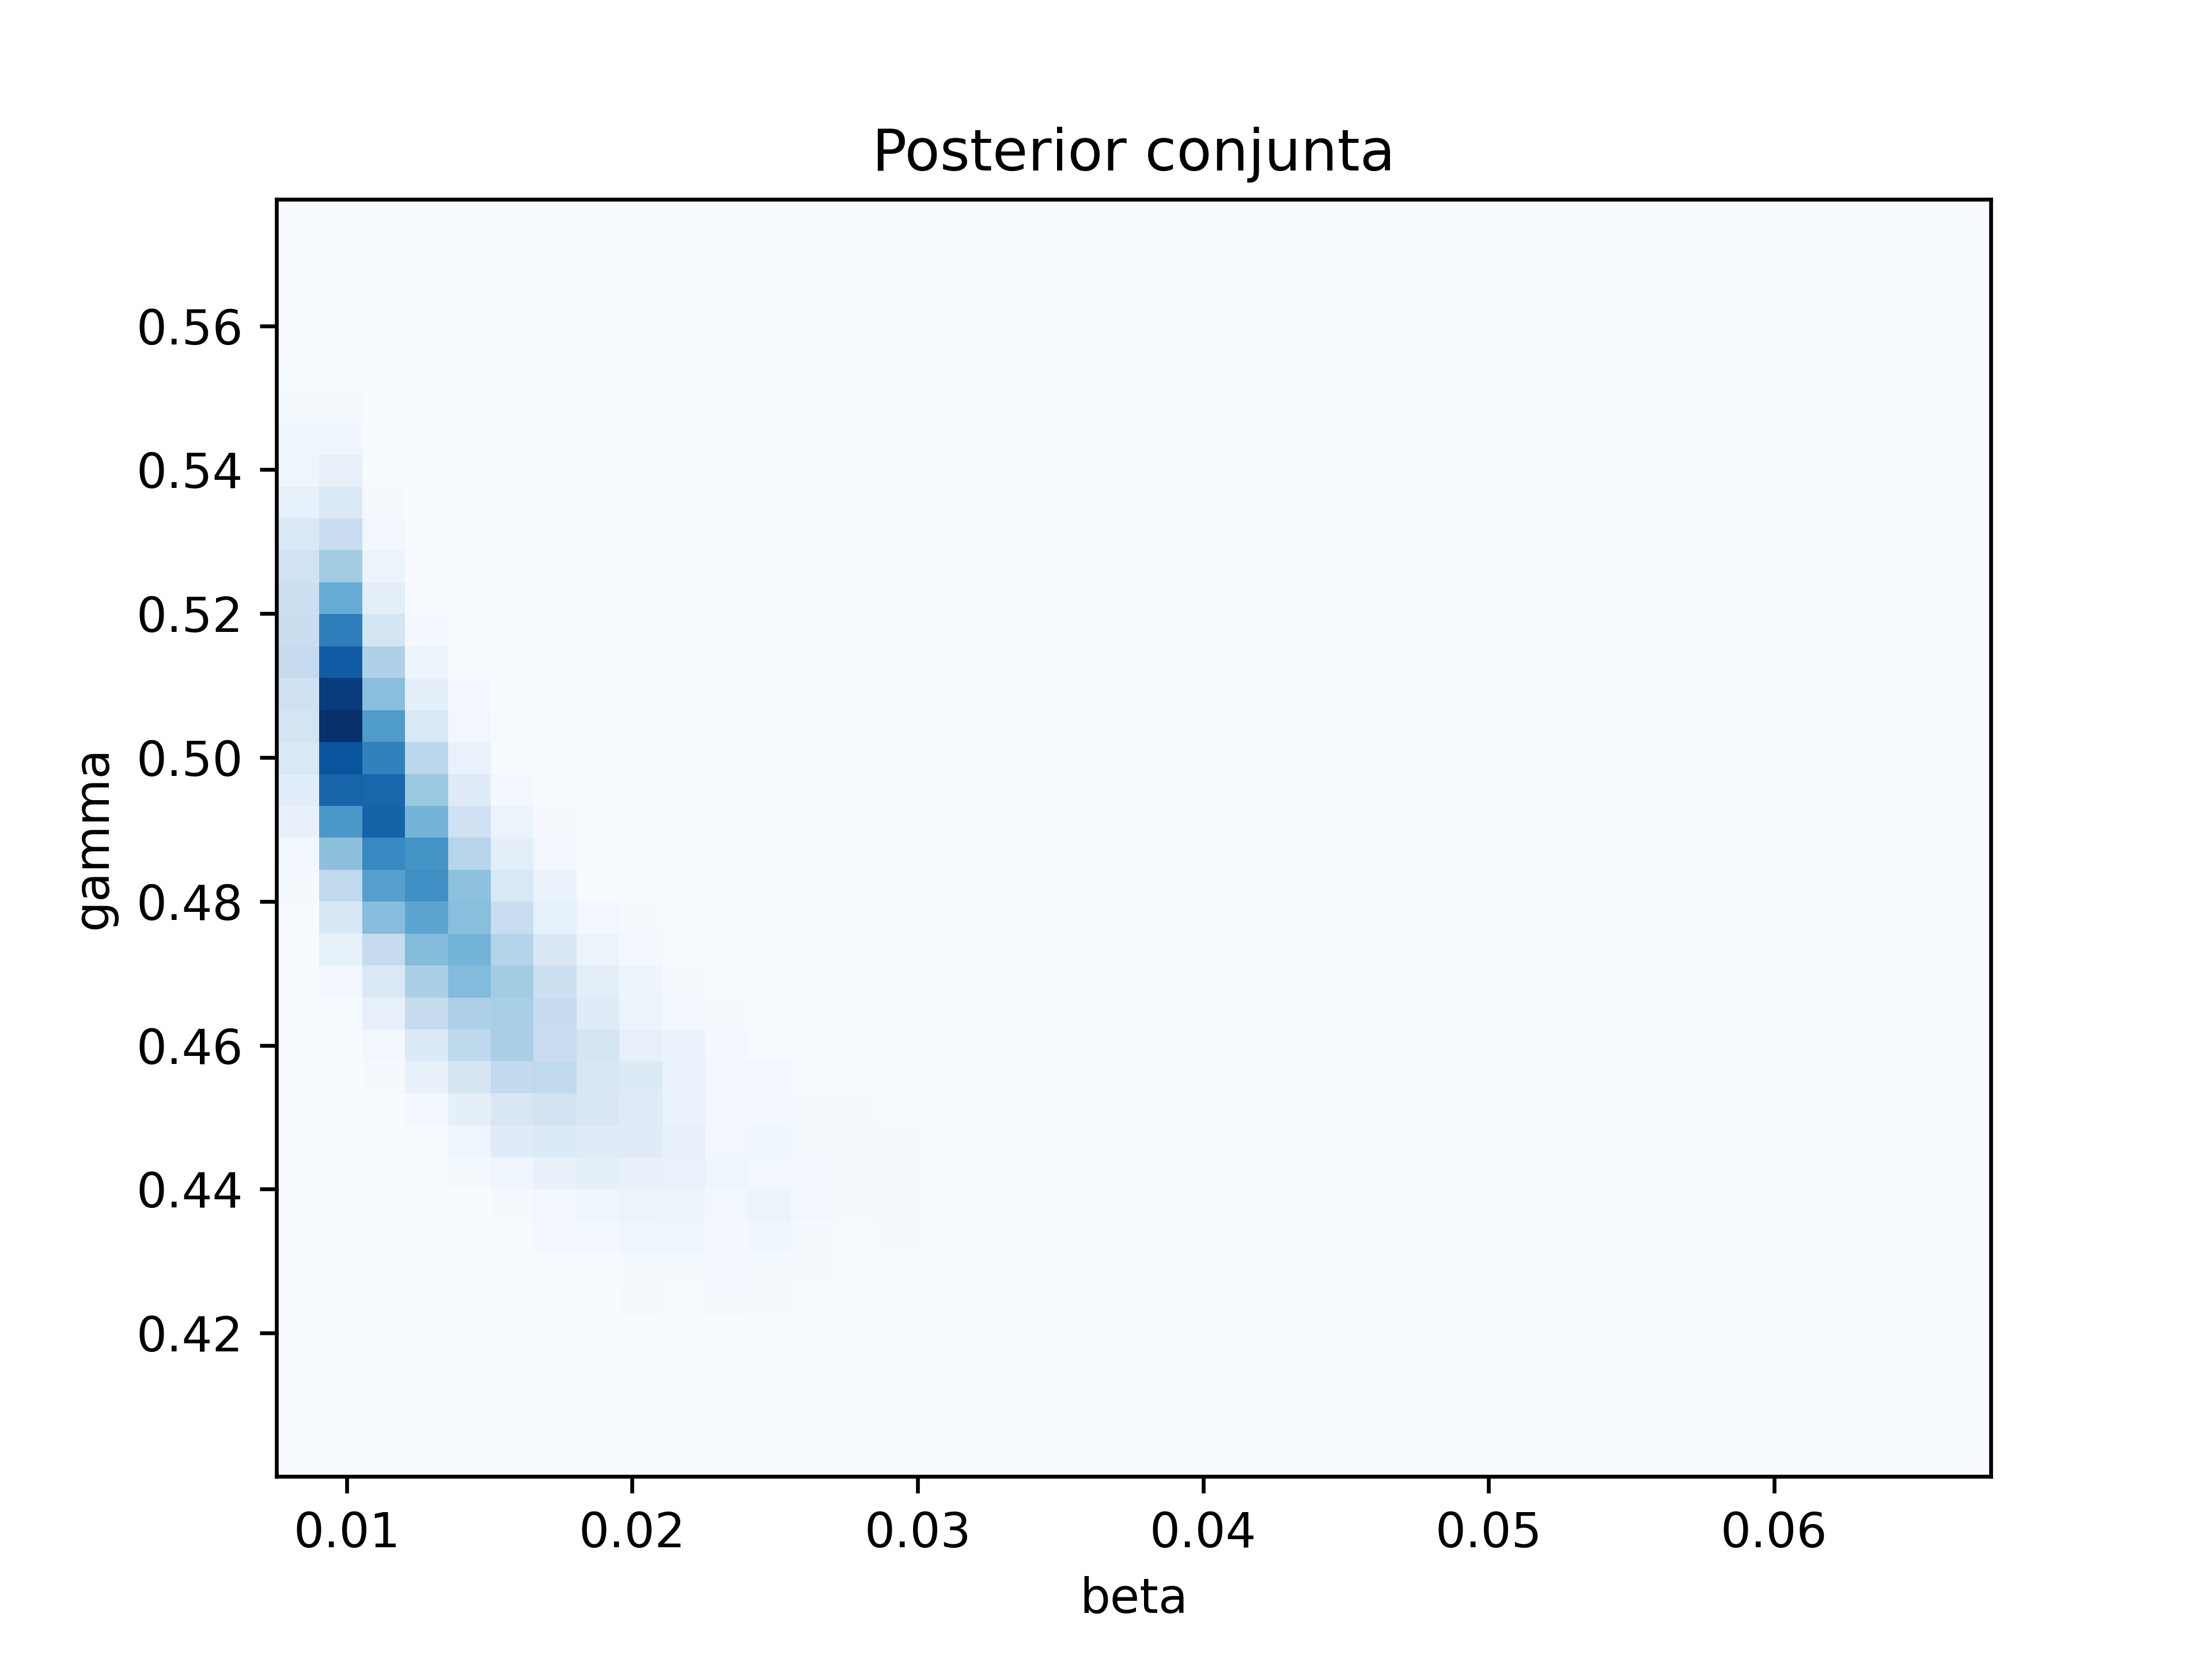
\includegraphics[width = 9 cm]{img/Exp_Central_SIR_sigma/Figuras/Generales/Conjunta_SIR_sigma.png} 
%     % \caption{Distribución posterior conjunta para el modelo SIR.}
%     \label{Fig. SIR_03}
%   \end{figure} 
% \end{frame}

% \begin{frame}{Simulación del Modelo SIR}
%   \begin{columns}[T,onlytextwidth]
%     \column{0.5\textwidth}
    
%     \begin{figure}
%       \centering 
%       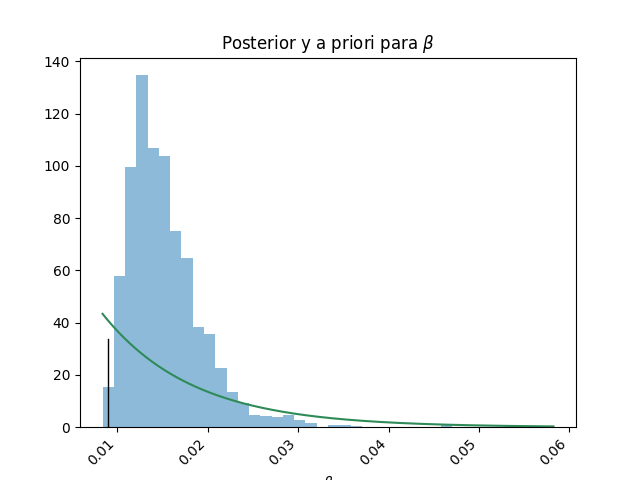
\includegraphics[width=0.9\textwidth]{img/Exp_Central_SIR_sigma/Figuras/Generales/Post_theta1_SIR_sigma.png}
%     \end{figure} 
    
%     \column{0.5\textwidth}
    
%       % \metroset{block=fill}
      
%     \begin{figure}
%       \centering 
%       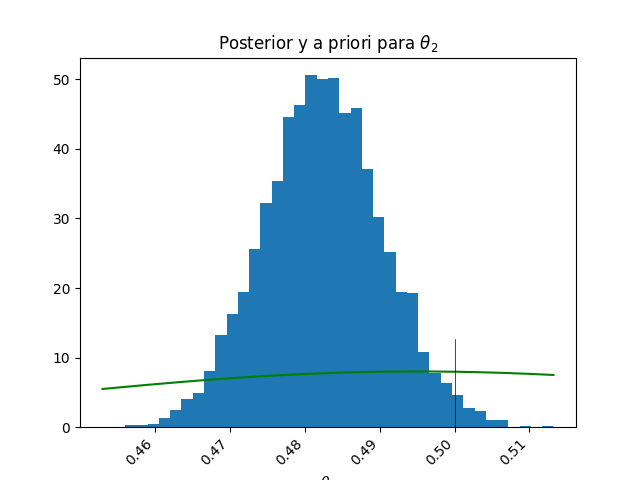
\includegraphics[width=0.9\textwidth]{img/Exp_Central_SIR_sigma/Figuras/Generales/Post_theta2_SIR_sigma.png}
%     \end{figure} 
    
%   \end{columns}
% \end{frame}

% \begin{frame}{Simulación del Modelo SIR}
  
%   \begin{figure}[H] 
%     \centering 
%     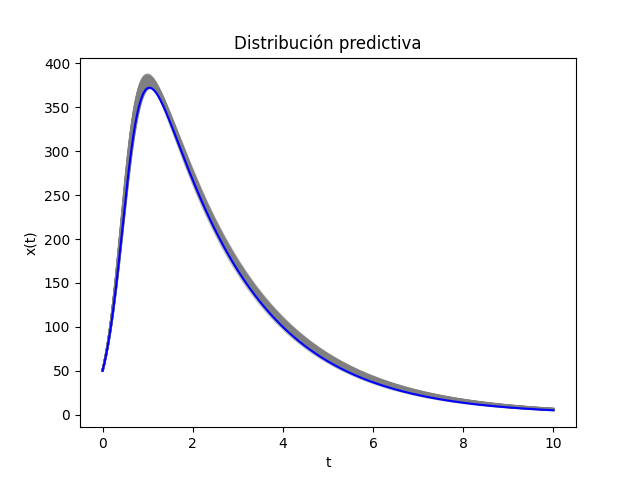
\includegraphics[width = 10 cm ]{img/Exp_Central_SIR_sigma/Figuras/Generales/Predictiva_SIR_sigma.png} 
%     % \caption{Distribución predictiva para el modelo SIR.}
%     \label{Fig. SIR_06}
%   \end{figure} 
% \end{frame}


\begin{frame}{Simulación con Forward Map Aproximado}
  Recordemos la construcción del \textbf{forward map aproximado}. Sea $\vartheta \in \mathcal{M}$. Sea $\vartheta^{(1)},\cdots, \vartheta^{(k)}$ los $k$ vecinos mas cercanos a $\theta$. Para $\theta \notin \mathcal{M}$ el forward map aproximado a $k$ vecinos cercanos de resolución $M$ es:
  \begin{align}
      \tilde{F}^{k}_M(\theta) = \sum_{j = 1}^{k} \omega_j(\theta) F \left(\vartheta^{(j)}\right)
      \label{3.3.01}
  \end{align}
  donde $\omega_j(\theta) = d_j(\theta)^{-1}/ \sum_{i=1}^{k} d_i(\theta)^{-1}$ con $d_j = d(\theta,\vartheta^{(j)})$ .
\end{frame}


\begin{frame}{Regularización de las Unidades}

  La regularización de la unidades es una aporte fundamental en la metodología del enfoque bayesiano del problema inverso con el forward map aproximado.

  \vspace{0.5 cm}

  Las distribuciones posteriores aproximadas son sensibles a las unidades de medida de las observables.

  \vspace{0.5 cm}
  
  Las unidades del modelo gravitatorio para $g$ usualmente se dan en $metros/segundo^2$ y para $b$ en $kilogramos/segundo$.
\end{frame}


\begin{frame}{Regularización de las Unidades}
  \begin{columns}[T,onlytextwidth]
    \column{0.5\textwidth}
    
    \begin{figure}
      \centering 
      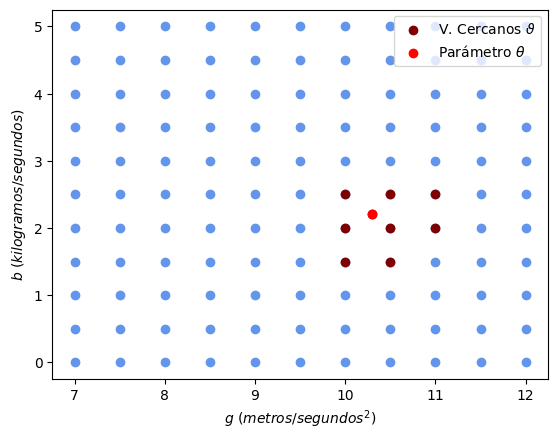
\includegraphics[width=0.9\textwidth]{img/Vecinos_1.png}
    \end{figure} 
    
    \column{0.5\textwidth}
    
      % \metroset{block=fill}
      
    \begin{figure}
      \centering 
      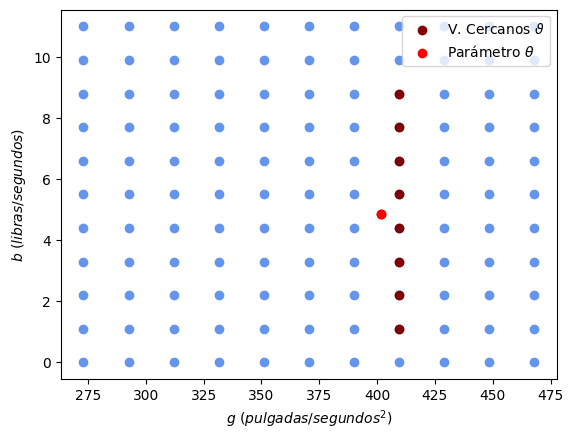
\includegraphics[width=0.9\textwidth]{img/Vecinos_2.png}
    \end{figure} 
    
  \end{columns}
\end{frame}

\begin{frame}{Regularización de las Unidades}
  La regularización de las unidades se establece como una técnica para normalizar cada parámetro al intervalo $[0,1]$. 

  Para cada componente de $\theta$, aplicamos la transformación de normalización $\varphi$ a la malla $\mathcal{M}$, donde a cada elemento $\theta_i^{(j)}\in \mathcal{M}_i$ se aplica la transformación
  \begin{align}
      \varphi_i^{(j)} = \frac{\theta_i^{(j)} - \theta_i^{Min}}{\theta_i^{Max}-\theta_i^{Min}}.
      \label{3.3.02}
  \end{align}

  Considerando que $\mathcal{N}_i = \{\varphi_i^{(1)},\cdots, \varphi_i^{(M)}\}$ para cada $i \in \{1,\cdots,d\}$.  De forma que se crea un enmallado uniforme $\mathcal{N} = \mathcal{N}_1 \times \cdots \times \mathcal{N}_d$.
\end{frame}

\begin{frame}{Experimentación con Distribuciones Posteriores Aproximadas}

  Las aproximaciones de la distribución posterior considera aproximaciones del forward map. 
  
  \begin{itemize}
    \item 
    Se experimentó con vecinos $k = 3,5,8$. 
    \item 
    Se aproxima el forward map con mallas de tamaño $M \times M$ con $M = 10, 15, 30, 50$.
  \end{itemize}

\end{frame}

\begin{frame}{Forward Map Aproximado para el Modelo Gravitatorio}

  Esta vez el análisis bayesiano se hará con el forward map aproximados para cada par $k$ y $M$ de las aproximaciones propuestas. 
  
  \vspace{0.5 cm}

  Posteriormente, las distribuciones aproximadas $\tilde{\pi}^{k}_M(g,b|\mathbf{y})$ las cotejaremos con su análogo ordinario, $\pi(g,b|\mathbf{y})$ de forma que sea visible o no la convergencia al análogo ordinario.
  
\end{frame}



\begin{frame}{Forward Map Aproximado para el Modelo Gravitatorio}
  \begin{figure}[H] 
    \centering 
    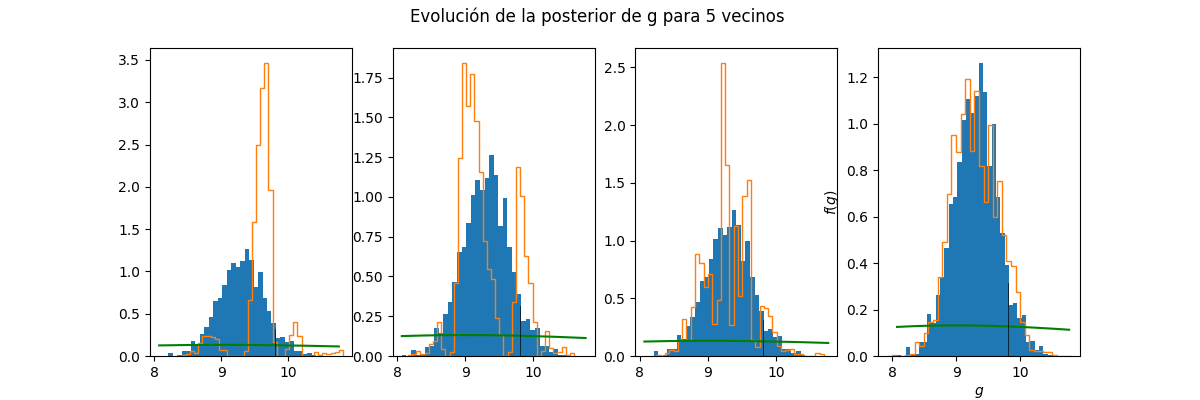
\includegraphics[width = 12 cm ]{img/Exp_Central_gravedad_Sigma/Figuras/Generales/Convergencia_theta1_1_gravedad_sigma.png} 
  \end{figure} 
  \begin{figure}[H] 
    \centering 
    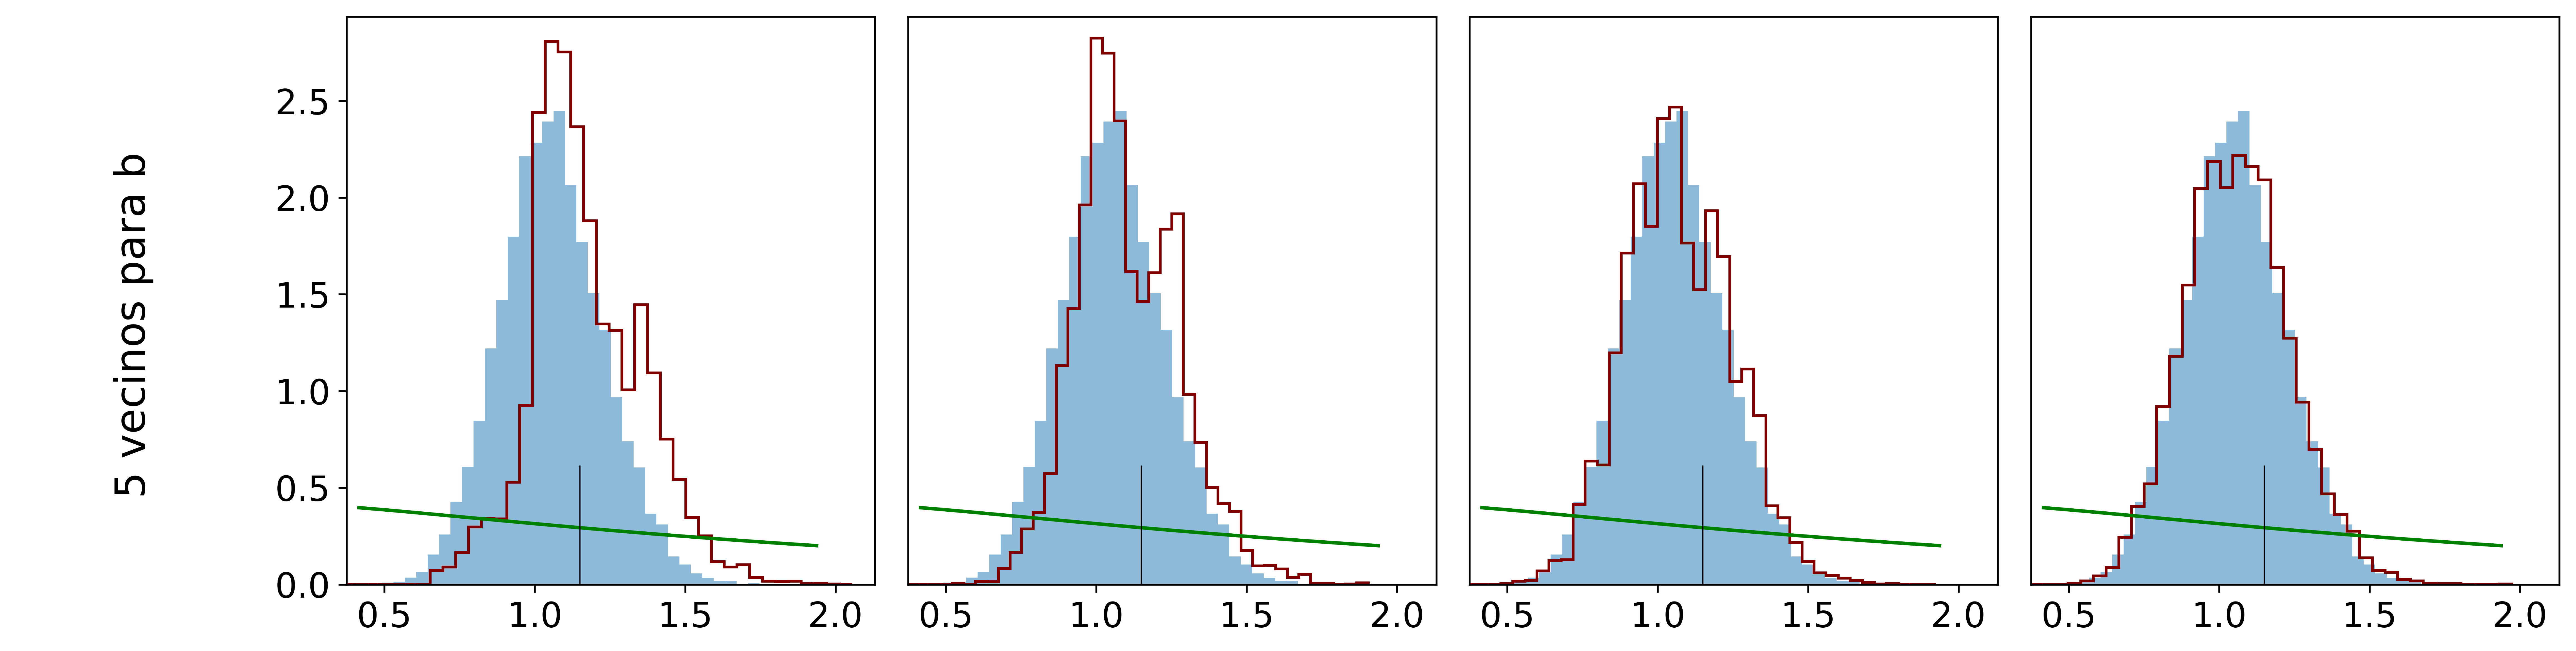
\includegraphics[width = 12 cm ]{img/Exp_Central_gravedad_Sigma/Figuras/Generales/Convergencia_theta2_1_gravedad_sigma.png} 
    % \caption{Distribuciones marginales posteriores aproximadas (rojo) con forward map aproximado a tres vecinos cercanos y una malla de resolución 10,15,30,50 de izquierda a derecha. En azul la distribución posterior con forward map ordinario para modelo gravitacional.}
    \label{Fig. Aprox grav 3v}
  \end{figure} 
\end{frame}

\begin{frame}{Forward Map Aproximado para el Modelo Gravitatorio}
  \begin{figure}[H] 
    \centering 
    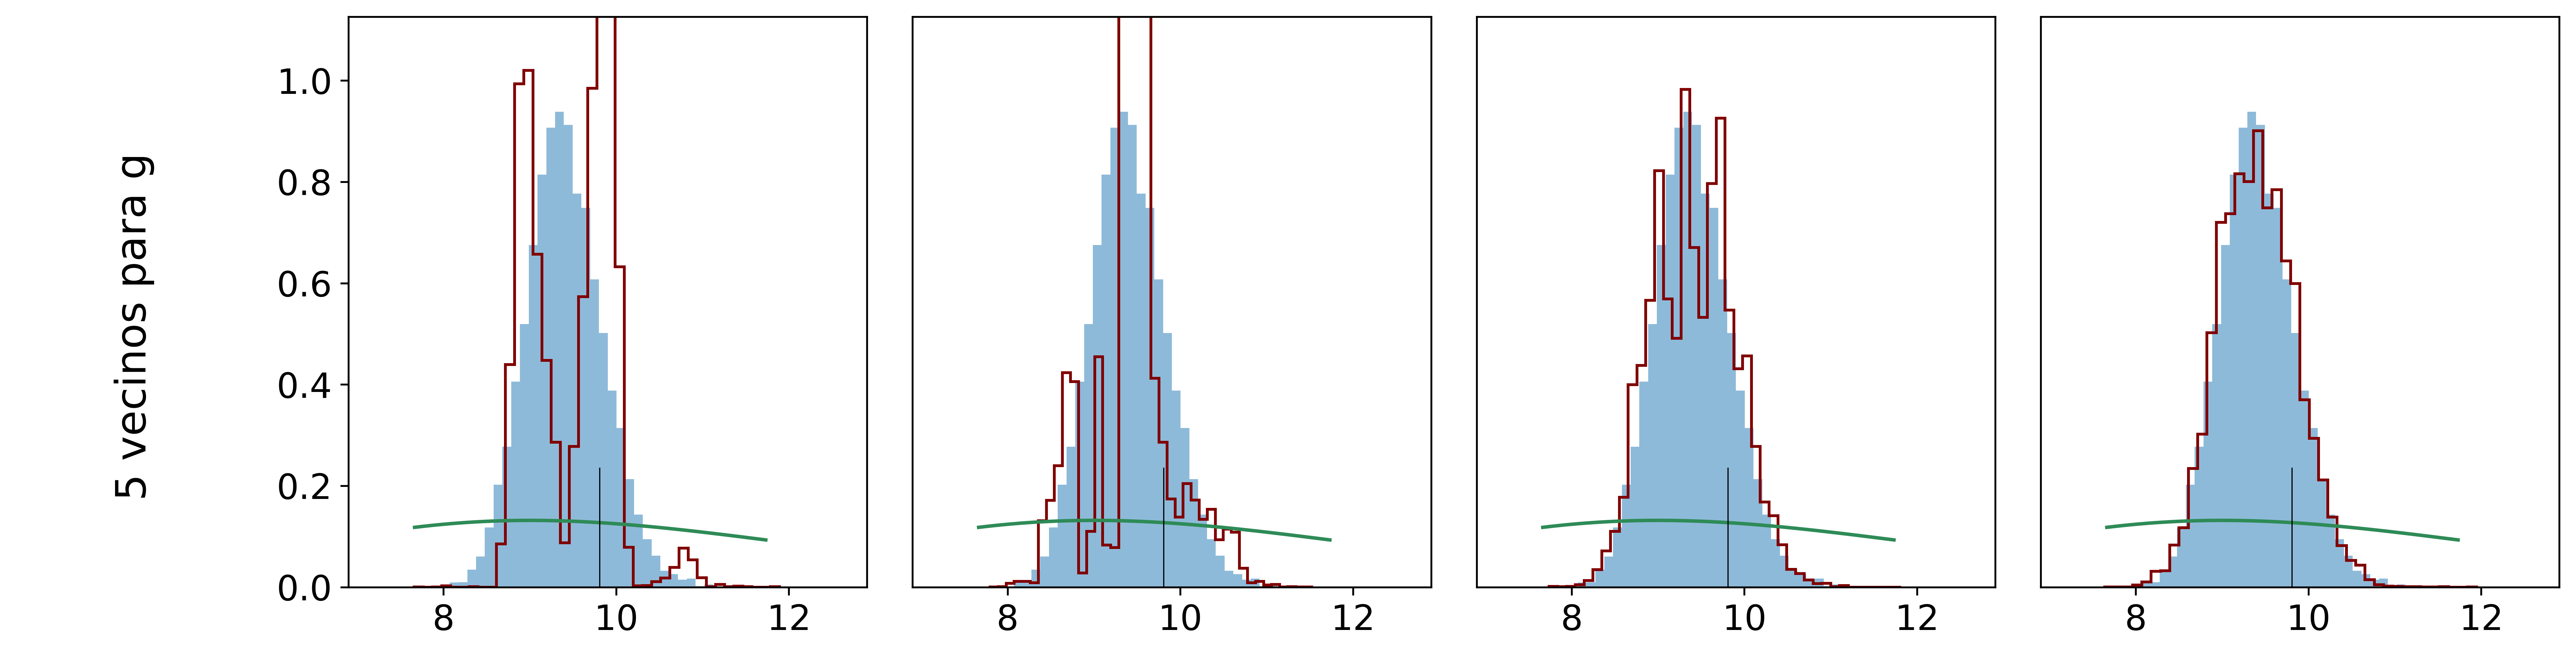
\includegraphics[width = 12 cm ]{img/Exp_Central_gravedad_Sigma/Figuras/Generales/Convergencia_theta1_2_gravedad_sigma.png} 
    % \caption{}
    % \label{Fig. }
  \end{figure} 
  
  \begin{figure}[H] 
    \centering 
    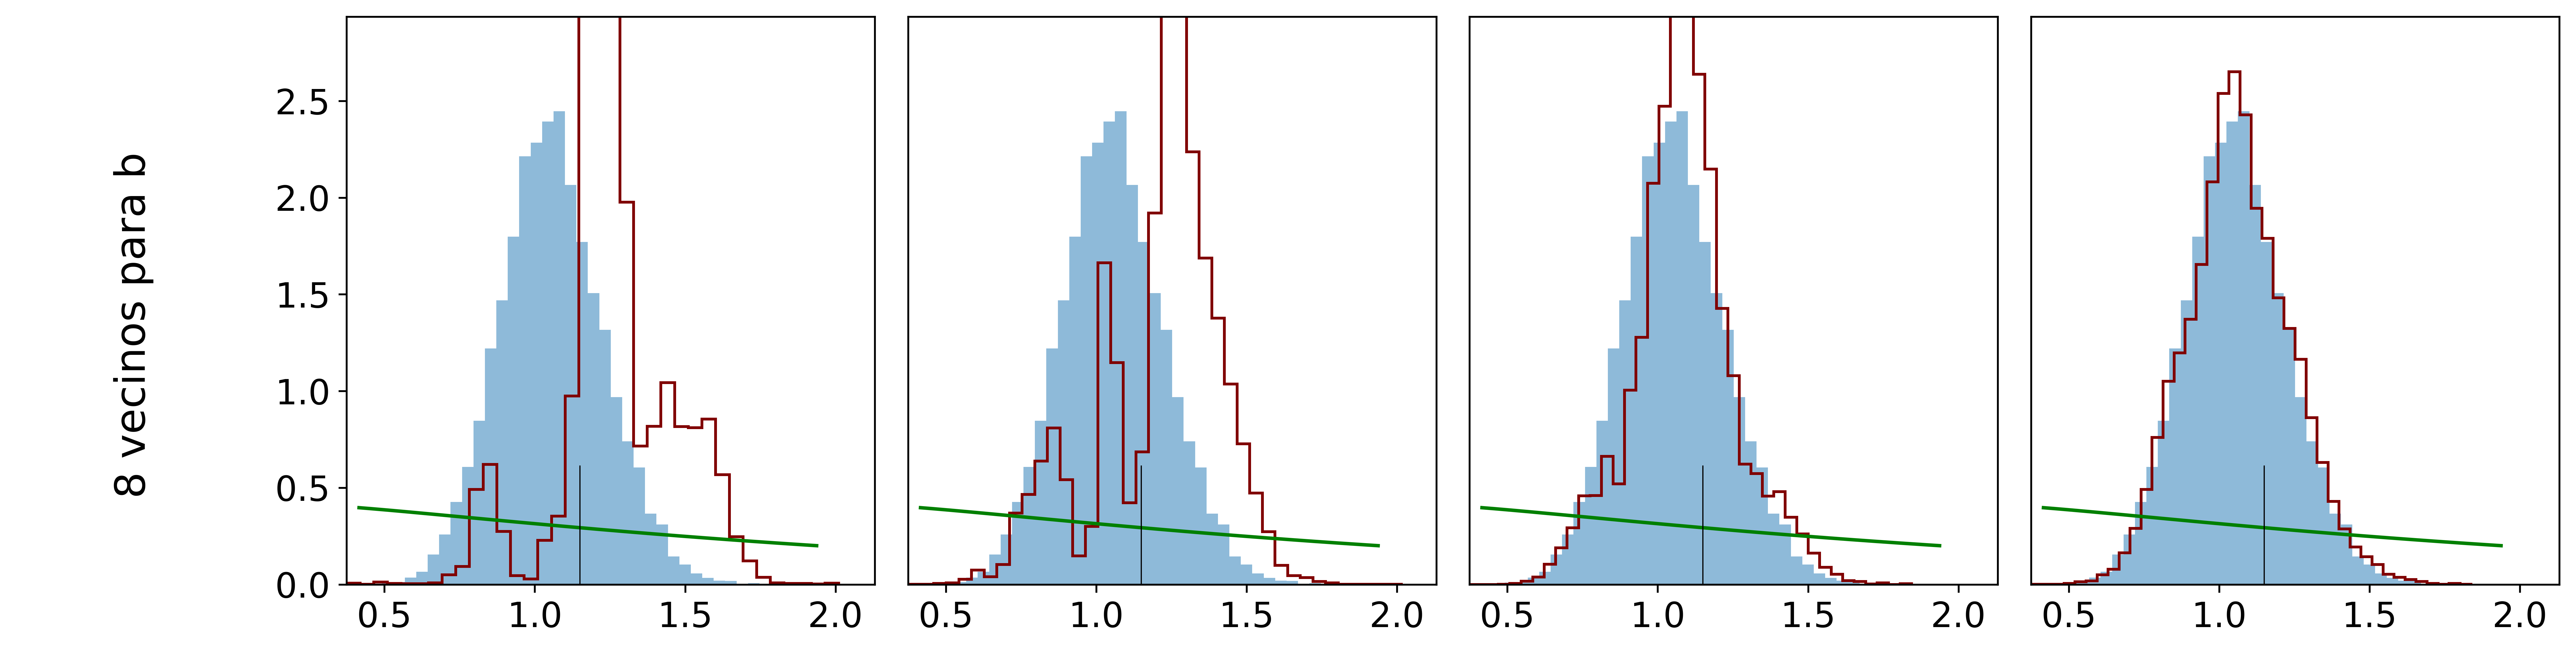
\includegraphics[width = 12 cm ]{img/Exp_Central_gravedad_Sigma/Figuras/Generales/Convergencia_theta2_2_gravedad_sigma.png} 
    % \caption{Distribuciones marginales posteriores aproximadas (rojo) con forward map aproximado a cinco vecinos cercanos y una malla de resolución 10,15,30,50 de izquierda a derecha. En azul la distribución posterior con forward map ordinario para modelo gravitacional.}
    \label{Fig. Aprox grav 5v}
  \end{figure} 
\end{frame}

\begin{frame}{Forward Map Aproximado para el Modelo Gravitatorio}
  \begin{figure}[H] 
    \centering 
    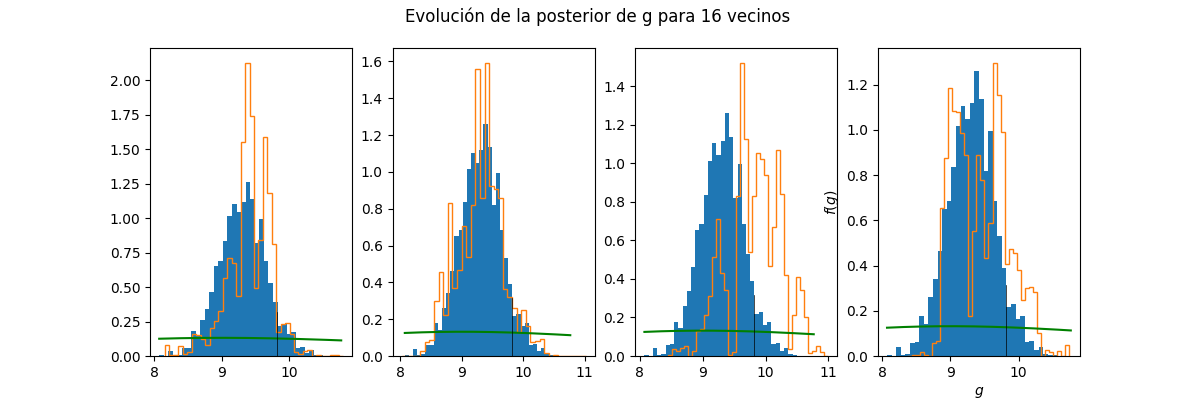
\includegraphics[width = 12 cm ]{img/Exp_Central_gravedad_Sigma/Figuras/Generales/Convergencia_theta1_3_gravedad_sigma.png} 
    % \caption{}
    % \label{Fig. }
  \end{figure} 
  \begin{figure}[H] 
    \centering 
    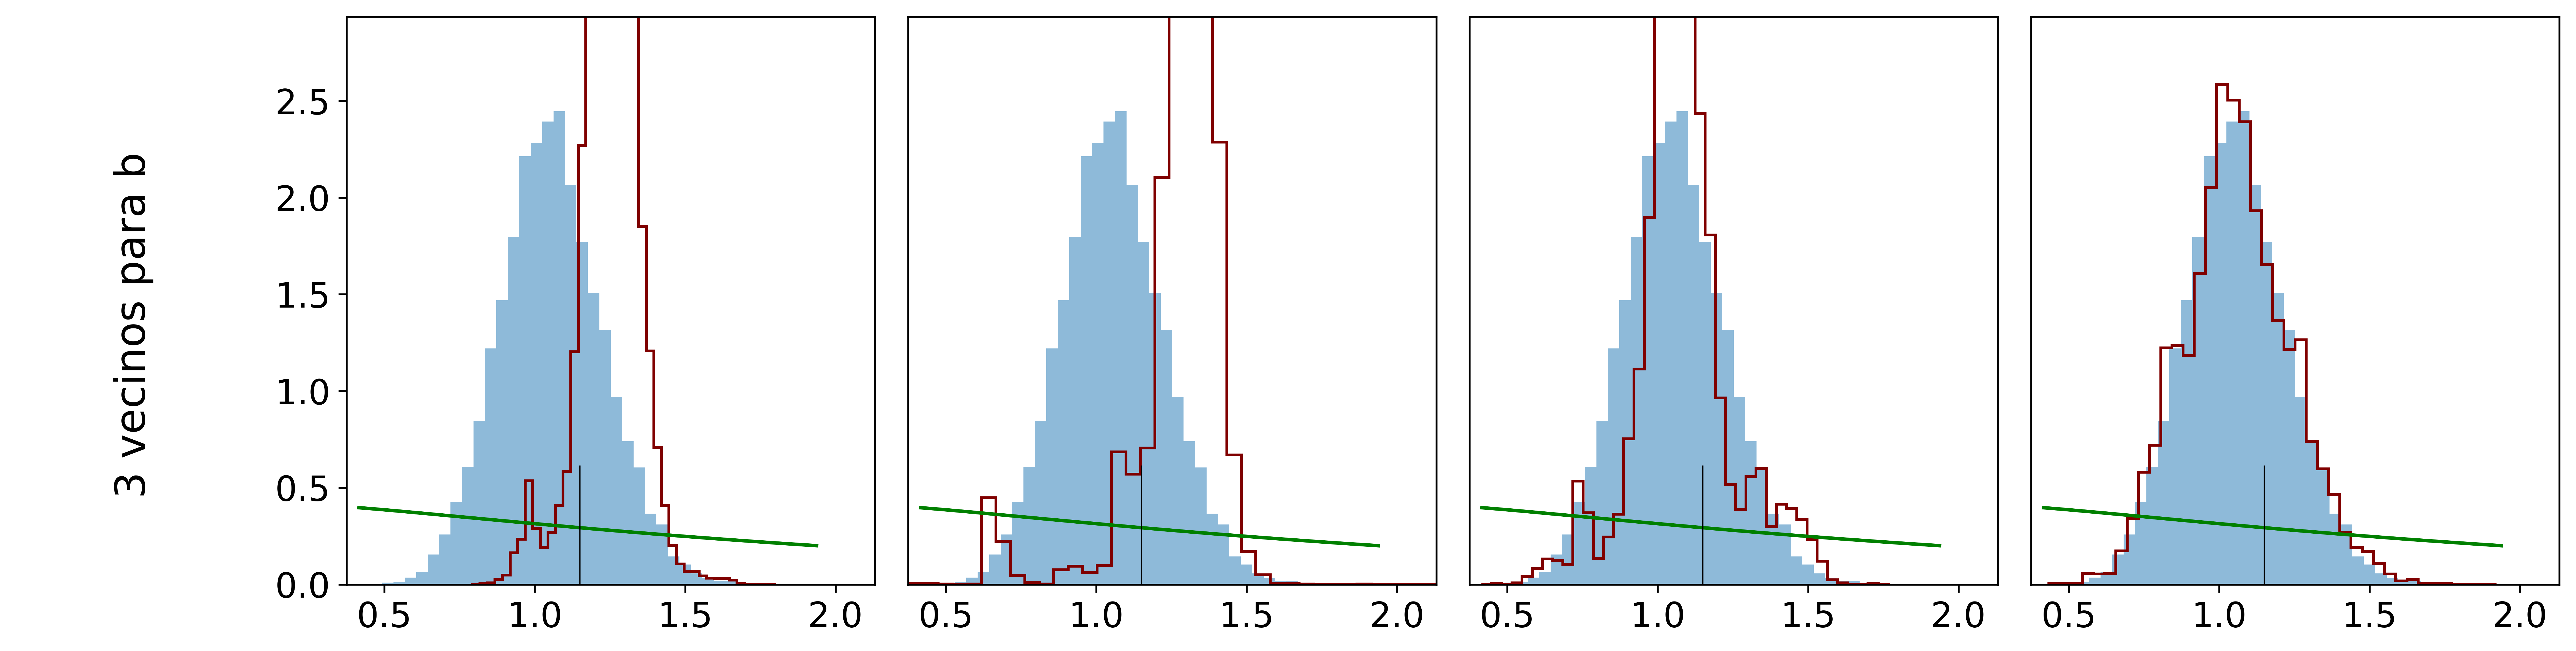
\includegraphics[width = 12 cm ]{img/Exp_Central_gravedad_Sigma/Figuras/Generales/Convergencia_theta2_3_gravedad_sigma.png} 
    % \caption{Distribuciones marginales posteriores aproximadas (rojo) con forward map aproximado a ocho vecinos cercanos y una malla de resolución 10,15,30,50 de izquierda a derecha. En azul la distribución posterior con forward map ordinario para modelo gravitacional.}
    \label{Fig. Aprox grav 8v}
  \end{figure} 
\end{frame}


\begin{frame}{Forward Map Aproximado para el Modelo Gravitatorio}
  El tiempo de ejecución del método ordinario para el problema inverso en el modelo gravitacional es de \textbf{5 min 57 s}.

  \vspace{0.5 cm}

  Tabla de tiempos de ejecución para el MCMC del modelo gravitatorio con forward map aproximado
  \begin{table}[H]
    \centering
    \begin{tabular}{l r r r c}
      \toprule
       \textbf{Malla} & \textbf{\:\:\:\:\:\:\:10 x 10\:\:\:\:\:\:\:} & \textbf{\:\:\:\:\:\:\:15 x 15\:\:\:\:\:\:\:} & \textbf{\:\:\:\:\:\:\:30 x 30\:\:\:\:\:\:\:} & \textbf{\:\:\:\:\:\:\:50 x 50\:\:\:\:\:\:\:} \\
      \midrule
      3 vecinos & 4m 52s & 4m 55s & 5m 52s & \textbf{5m 00s}\\
      5 vecinos & 5m 03s & 5m 02s & 4m 53s & 5m 02s\\
      8 vecinos & 5m 00s & 5m 09s & 5m 02s & 5m 02s\\
      \bottomrule
    \end{tabular}
    % \caption{Tabla de tiempos de ejecución para el MCMC del modelo gravitatorio con forward map aproximado con $k$ vecinos (filas) en una malla de $M\times M$ (columnas).}
    \label{tabla_01}
  \end{table}
\end{frame}

\begin{frame}{Forward Map Aproximado para el Modelo Logístico}
  \begin{figure}[H] 
    \centering 
    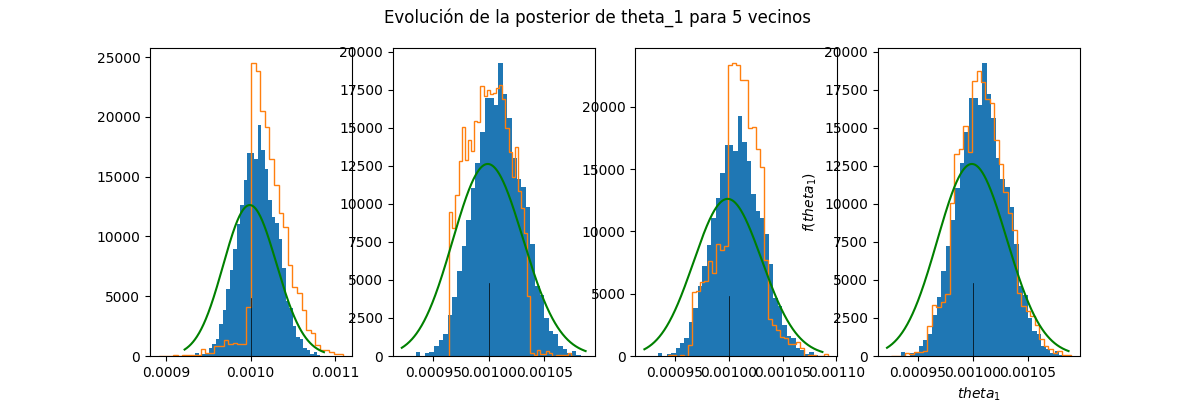
\includegraphics[width = 12 cm ]{img/Exp_Central_logistico_Sigma/Figuras/Generales/Convergencia_theta1_1_logistico_sigma.png} 
    % \caption{}
    % \label{Fig. }
  \end{figure} 
  \begin{figure}[H] 
    \centering 
    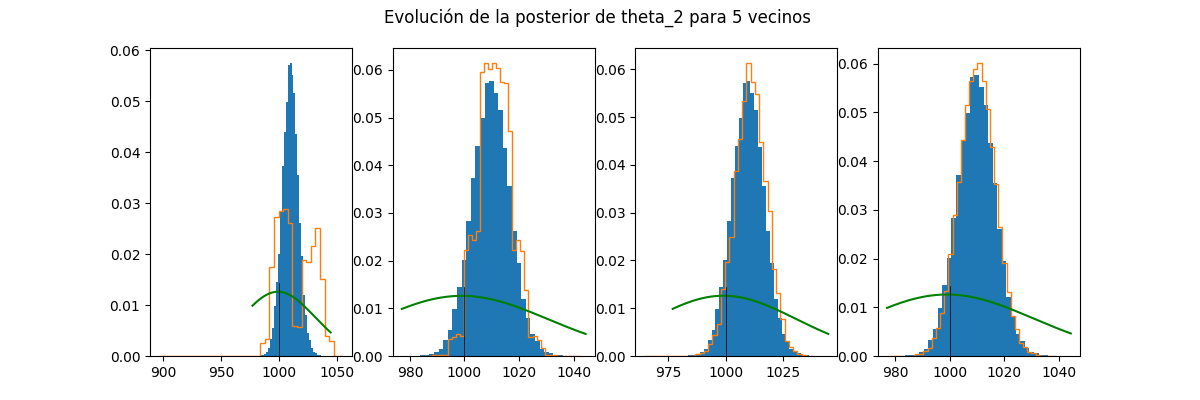
\includegraphics[width = 12 cm ]{img/Exp_Central_logistico_Sigma/Figuras/Generales/Convergencia_theta2_1_logistico_sigma.png} 
    % \caption{Distribuciones marginales posteriores aproximadas (rojo) con forward map aproximado a tres vecinos cercanos y una malla de resolución 10,15,30,50 de izquierda a derecha. En azul la distribución posterior con forward map ordinario para modelo logístico.}
    \label{Fig. Aprox log 3v}
  \end{figure} 
\end{frame}


\begin{frame}{Forward Map Aproximado para el Modelo Logístico}
  \begin{figure}[H] 
    \centering 
    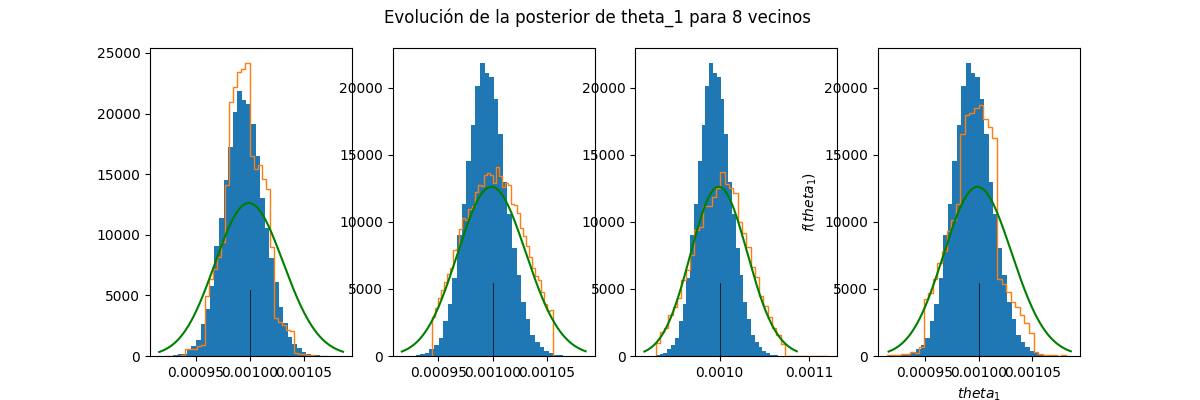
\includegraphics[width = 12 cm ]{img/Exp_Central_logistico_Sigma/Figuras/Generales/Convergencia_theta1_2_logistico_sigma.png} 
    % \caption{}
    % \label{Fig. }
  \end{figure} 
  \begin{figure}[H] 
    \centering 
    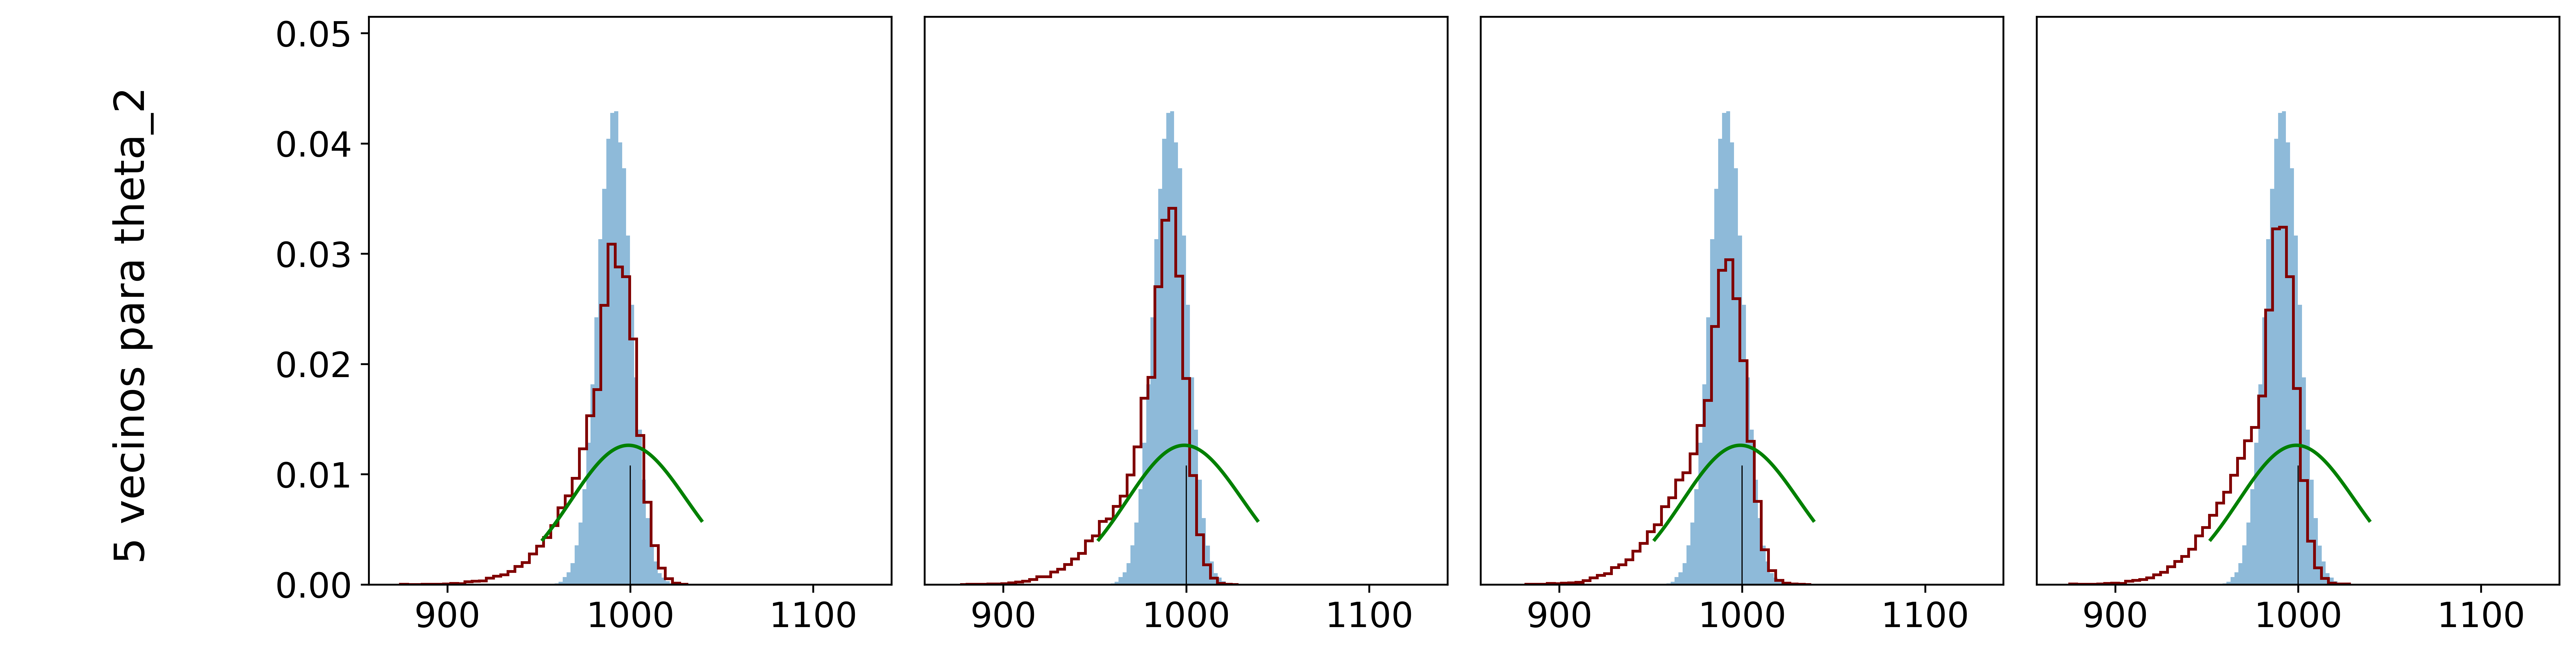
\includegraphics[width = 12 cm ]{img/Exp_Central_logistico_Sigma/Figuras/Generales/Convergencia_theta2_2_logistico_sigma.png} 
    % \caption{Distribuciones marginales posteriores aproximadas (rojo) con forward map aproximado a cinco vecinos cercanos y una malla de resolución 10,15,30,50 de izquierda a derecha. En azul la distribución posterior con forward map ordinario para modelo logístico.}
    \label{Fig. Aprox log 5v}
  \end{figure} 
\end{frame}


\begin{frame}{Forward Map Aproximado para el Modelo Logístico}
  \begin{figure}[H] 
    \centering 
    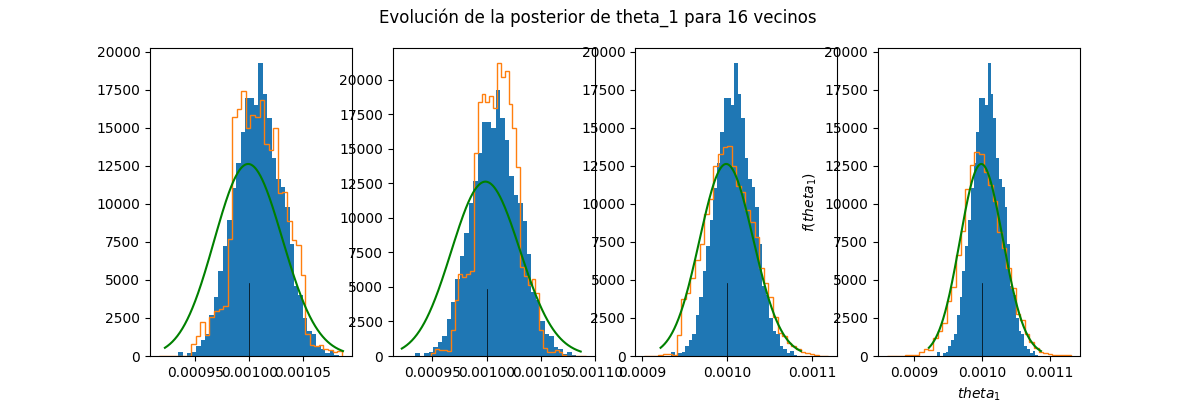
\includegraphics[width = 12 cm ]{img/Exp_Central_logistico_Sigma/Figuras/Generales/Convergencia_theta1_3_logistico_sigma.png} 
    % \caption{}
    % \label{Fig. }
\end{figure} 
\begin{figure}[H] 
  \centering 
  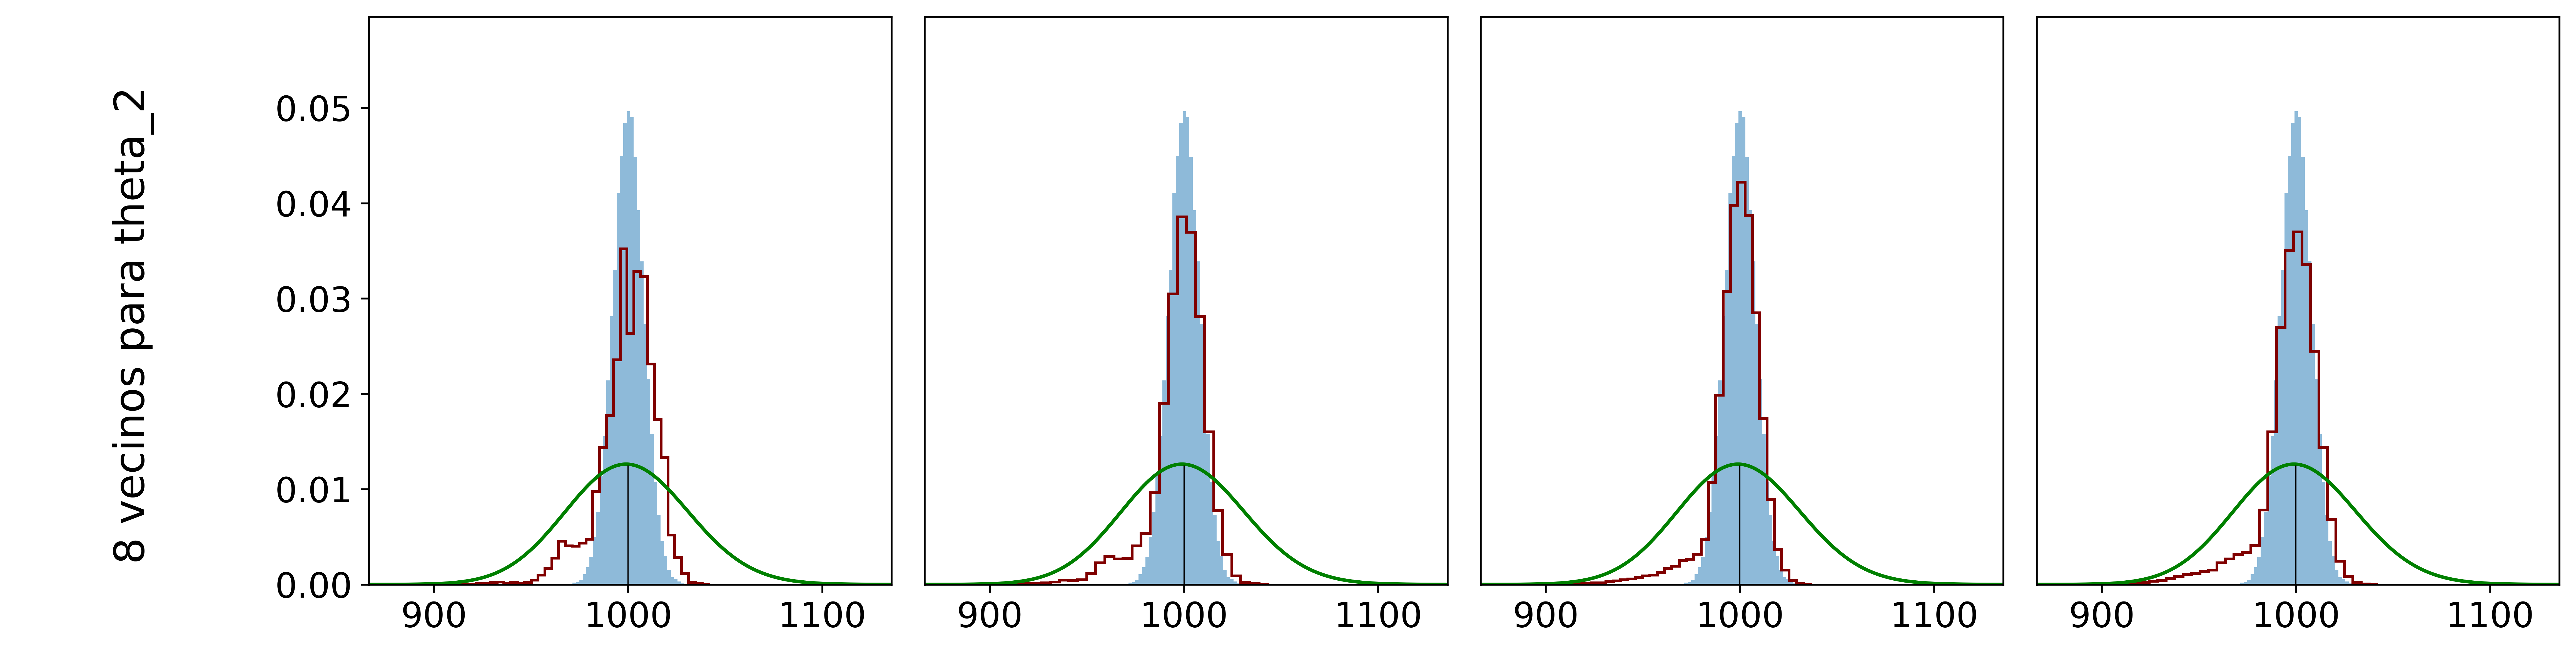
\includegraphics[width = 12 cm ]{img/Exp_Central_logistico_Sigma/Figuras/Generales/Convergencia_theta2_3_logistico_sigma.png} 
  % \caption{Distribuciones marginales posteriores aproximadas (rojo) con forward map aproximado a ocho vecinos cercanos y una malla de resolución 10,15,30,50 de izquierda a derecha. En azul la distribución posterior con forward map ordinario.}
  \label{Fig. Aprox log 8v}
  \end{figure} 
\end{frame}


\begin{frame}{Forward Map Aproximado para el Modelo Logístico}
  
  El tiempo de ejecución del método ordinario para el problema inverso en el modelo logístico es de \textbf{20 min 58 s}. 

  \vspace{0.5 cm}

  Tabla de tiempos de ejecución para el MCMC del modelo logístico con forward map aproximado
  \begin{table}[H]
    \centering
    \begin{tabular}{l r r r c}
      \toprule
       \textbf{Malla} & \textbf{\:\:\:\:\:\:\:10 x 10\:\:\:\:\:\:\:} & \textbf{\:\:\:\:\:\:\:15 x 15\:\:\:\:\:\:\:} & \textbf{\:\:\:\:\:\:\:30 x 30\:\:\:\:\:\:\:} & \textbf{\:\:\:\:\:\:\:50 x 50\:\:\:\:\:\:\:} \\
      \midrule
      3 vecinos & 10m 58s & 9m 36s & 9m 25s & \textbf{6m 02s}\\
      5 vecinos & 6m 02s & 6m 03s & 7m 20s & 10m 04s\\
      8 vecinos & 10m 08s & 10m 24s & 10m 21s & 10m 21s\\
      \bottomrule
    \end{tabular}
    % \caption{Tabla de tiempos de ejecución para el MCMC del modelo logístico con forward map aproximado con $k$ vecinos (filas) en una malla de $M\times M$ (columnas).}
    \label{tabla_02}
  \end{table}
\end{frame}

\begin{frame}{Forward Map Aproximado para el Modelo SIR}
  \begin{figure}[H] 
    \centering 
    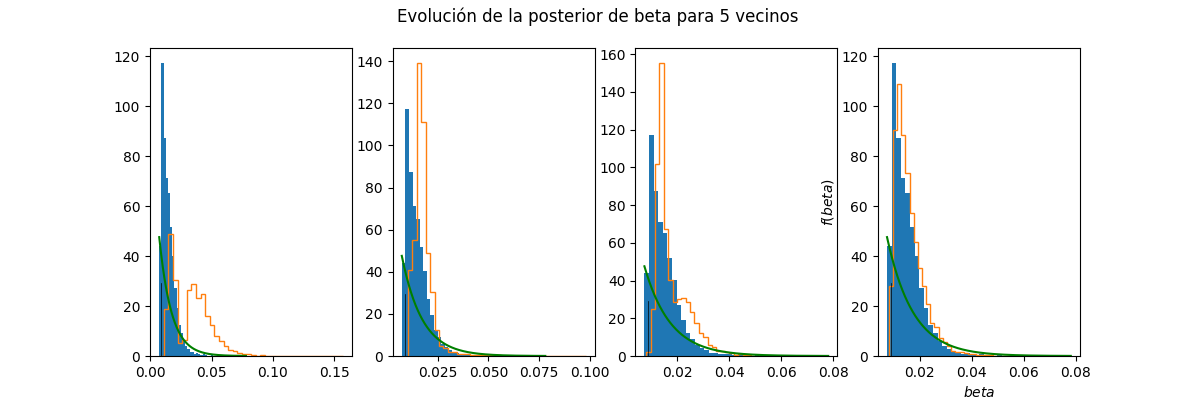
\includegraphics[width = 12 cm ]{img/Exp_Central_SIR_Sigma/Figuras/Generales/Convergencia_theta1_1_SIR_sigma.png} 
    % \caption{}
    % \label{Fig. }
  \end{figure} 
  \begin{figure}[H] 
    \centering 
    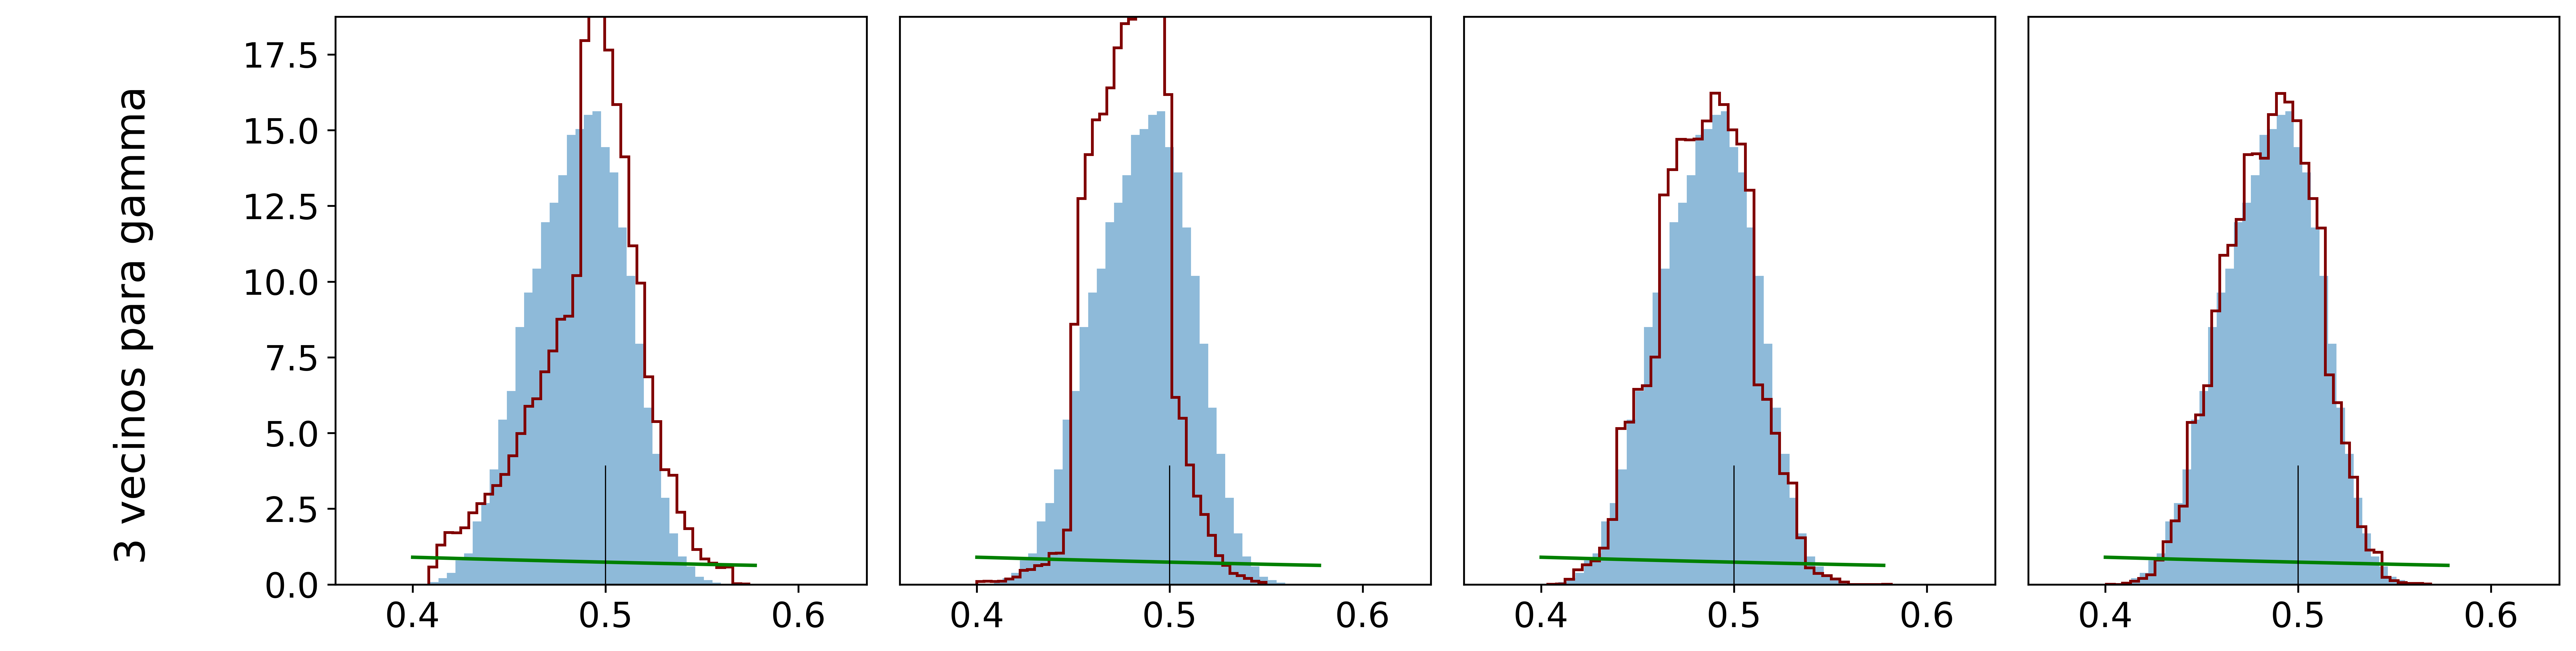
\includegraphics[width = 12 cm ]{img/Exp_Central_SIR_Sigma/Figuras/Generales/Convergencia_theta2_1_SIR_sigma.png}
    % \caption{Distribuciones marginales posteriores aproximadas (rojo) con forward map aproximado a tres vecinos cercanos y una malla de resolución 10,15,30,50 de izquierda a derecha. En azul la distribución posterior con forward map ordinario para modelo SIR.}
    \label{Fig. Aprox SIR 3v}
\end{figure} 
\end{frame}

\begin{frame}{Forward Map Aproximado para el Modelo SIR}
  \begin{figure}[H] 
    \centering 
    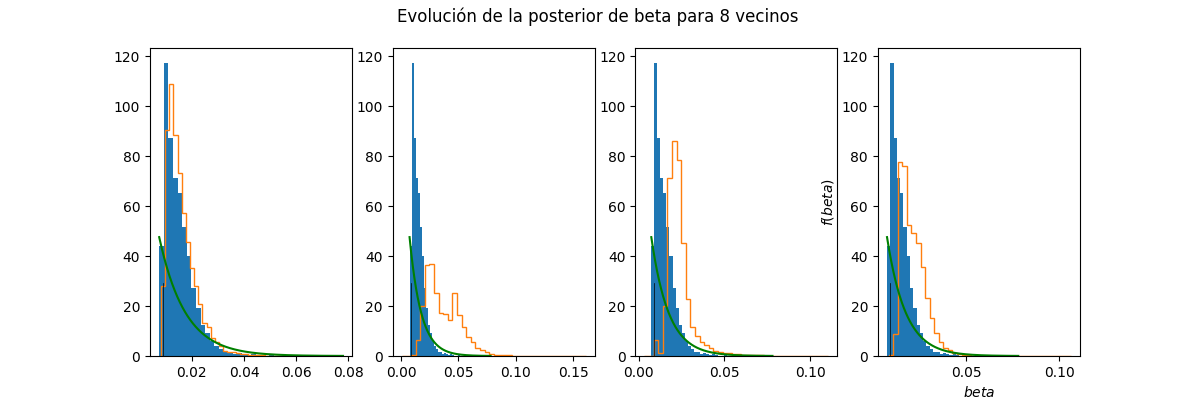
\includegraphics[width = 12 cm ]{img/Exp_Central_SIR_Sigma/Figuras/Generales/Convergencia_theta1_2_SIR_sigma.png} 
    % \caption{}
    % \label{Fig. }
  \end{figure} 
  \begin{figure}[H] 
    \centering 
    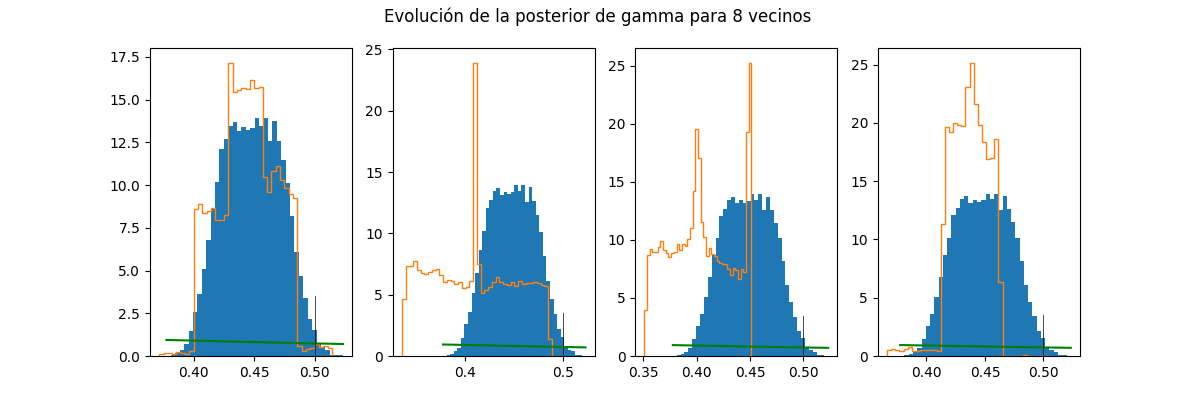
\includegraphics[width = 12 cm ]{img/Exp_Central_SIR_Sigma/Figuras/Generales/Convergencia_theta2_2_SIR_sigma.png} 
    % \caption{Distribuciones marginales posteriores aproximadas (rojo) con forward map aproximado a cinco vecinos cercanos y una malla de resolución 10,15,30,50 de izquierda a derecha. En azul la distribución posterior con forward map ordinario para modelo SIR.}
    \label{Fig. Aprox SIR 5v} 
  \end{figure} 
\end{frame}

\begin{frame}{Forward Map Aproximado para el Modelo SIR}
  \begin{figure}[H] 
    \centering 
    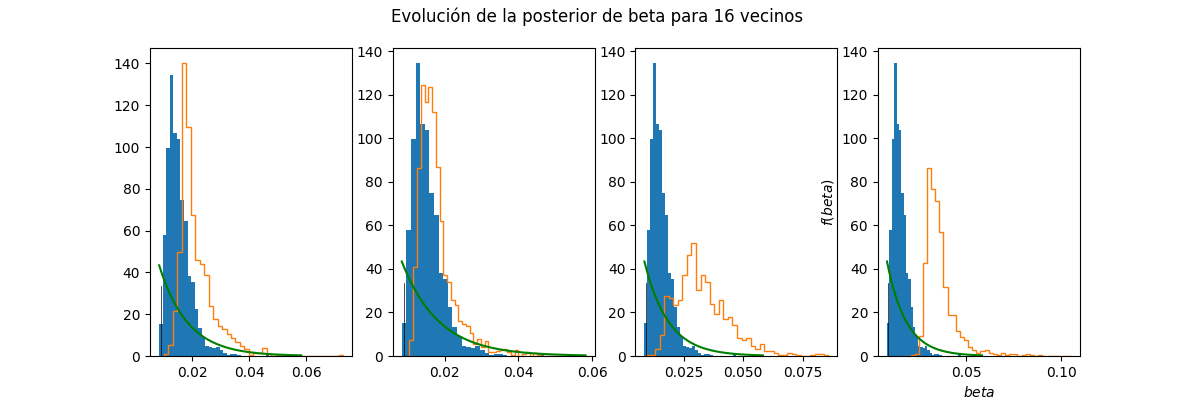
\includegraphics[width = 12 cm ]{img/Exp_Central_SIR_Sigma/Figuras/Generales/Convergencia_theta1_3_SIR_sigma.png} 
    % \caption{}
    % \label{Fig. }
  \end{figure} 
  \begin{figure}[H] 
    \centering 
    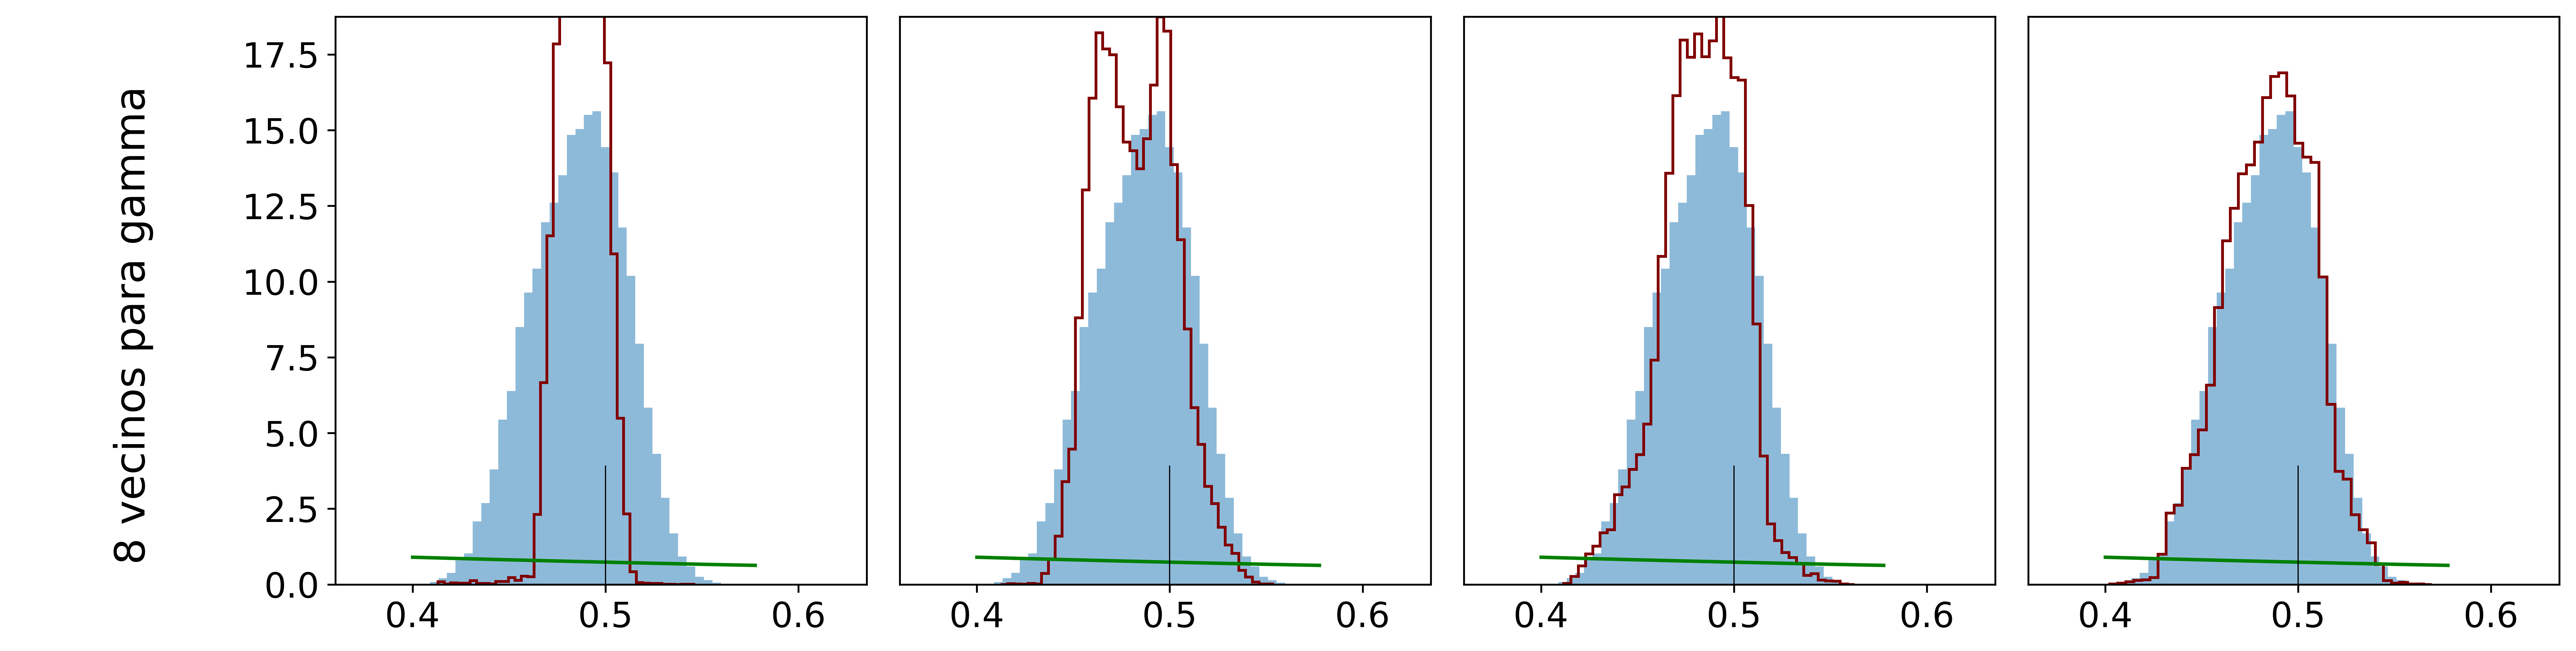
\includegraphics[width = 12 cm ]{img/Exp_Central_SIR_Sigma/Figuras/Generales/Convergencia_theta2_3_SIR_sigma.png} 
    % \caption{Distribuciones marginales posteriores aproximadas (rojo) con forward map aproximado a ocho vecinos cercanos y una malla de resolución 10,15,30,50 de izquierda a derecha. En azul la distribución posterior con forward map ordinario para modelo SIR.}
    \label{Fig. Aprox SIR 8v}
  \end{figure} 
\end{frame}

\begin{frame}{Forward Map Aproximado para el Modelo SIR}
  El tiempo de ejecución del método ordinario para el problema inverso en el modelo gravitacional es de \textbf{14 min 05 seg}.

  \vspace{0.5 cm}

  Tabla de tiempos de ejecución para el MCMC del modelo SIR con forward map aproximado
  \begin{table}[H]
    \centering
    \begin{tabular}{l r r r c}
      \toprule
      \textbf{Malla} & \textbf{\:\:\:\:\:\:\:10 x 10\:\:\:\:\:\:\:} & \textbf{\:\:\:\:\:\:\:15 x 15\:\:\:\:\:\:\:} & \textbf{\:\:\:\:\:\:\:30 x 30\:\:\:\:\:\:\:} & \textbf{\:\:\:\:\:\:\:50 x 50\:\:\:\:\:\:\:} \\
      \midrule
      3 vecinos & 5m 38s & 5m 36s & 8m 14s & \textbf{5m 50s}\\
      5 vecinos & 5m 59s & 5m 50s & 5m 56s & 5m 57s\\
      8 vecinos & 6m 38s & 7m 26s & 7m 02s & 6m 09s\\
      \bottomrule
    \end{tabular}
    \caption{Tabla de tiempos de ejecución para el MCMC del modelo SIR con forward map aproximado con $k$ vecinos (filas) en una malla de $M\times M$ (columnas).}
    \label{tabla_03}
  \end{table}
\end{frame}

\section{Conclusiones y Trabajo Futuro}

\begin{frame}{Conclusiones}
  \begin{enumerate}
    \item 
    Las aproximaciones de la distribución posterior dadas por las aproximaciones del forward map son en general útiles y simples de manejar.
    \item 
    En cada uno de los tres modelos estudiados se llegó a que existe una aproximación decente con un menor tiempo de ejecución.
    \item
    Aunque es cierto que comparaciones uno a uno el método aproximado es mejor en tiempo de ejecución, no lo es en conjunto.

    % \item Por razonamiento inductivo, podemos conjeturar que tendremos una aproximación decente en cualquier otro modelo de EDO's con tres vecinos cercanos y una definición de malla de 50.
  \end{enumerate}
\end{frame}


\begin{frame}{Conclusiones}
  En la práctica, el uso de la metodología sin la regularización de las unidades produce aproximaciones burdas para los parámetros con mayor orden de magnitud.

  \vspace{0.5 cm}

  En el caso del modelo SIR, considerar la resolución del problema inverso sin la regularización de las unidades, ocasiona que la distribución posterior aproximada, solo aproxima marginalmente para $\beta$.
\end{frame}


\begin{frame}{Conclusiones}
  \begin{figure}[H] 
    \centering 
    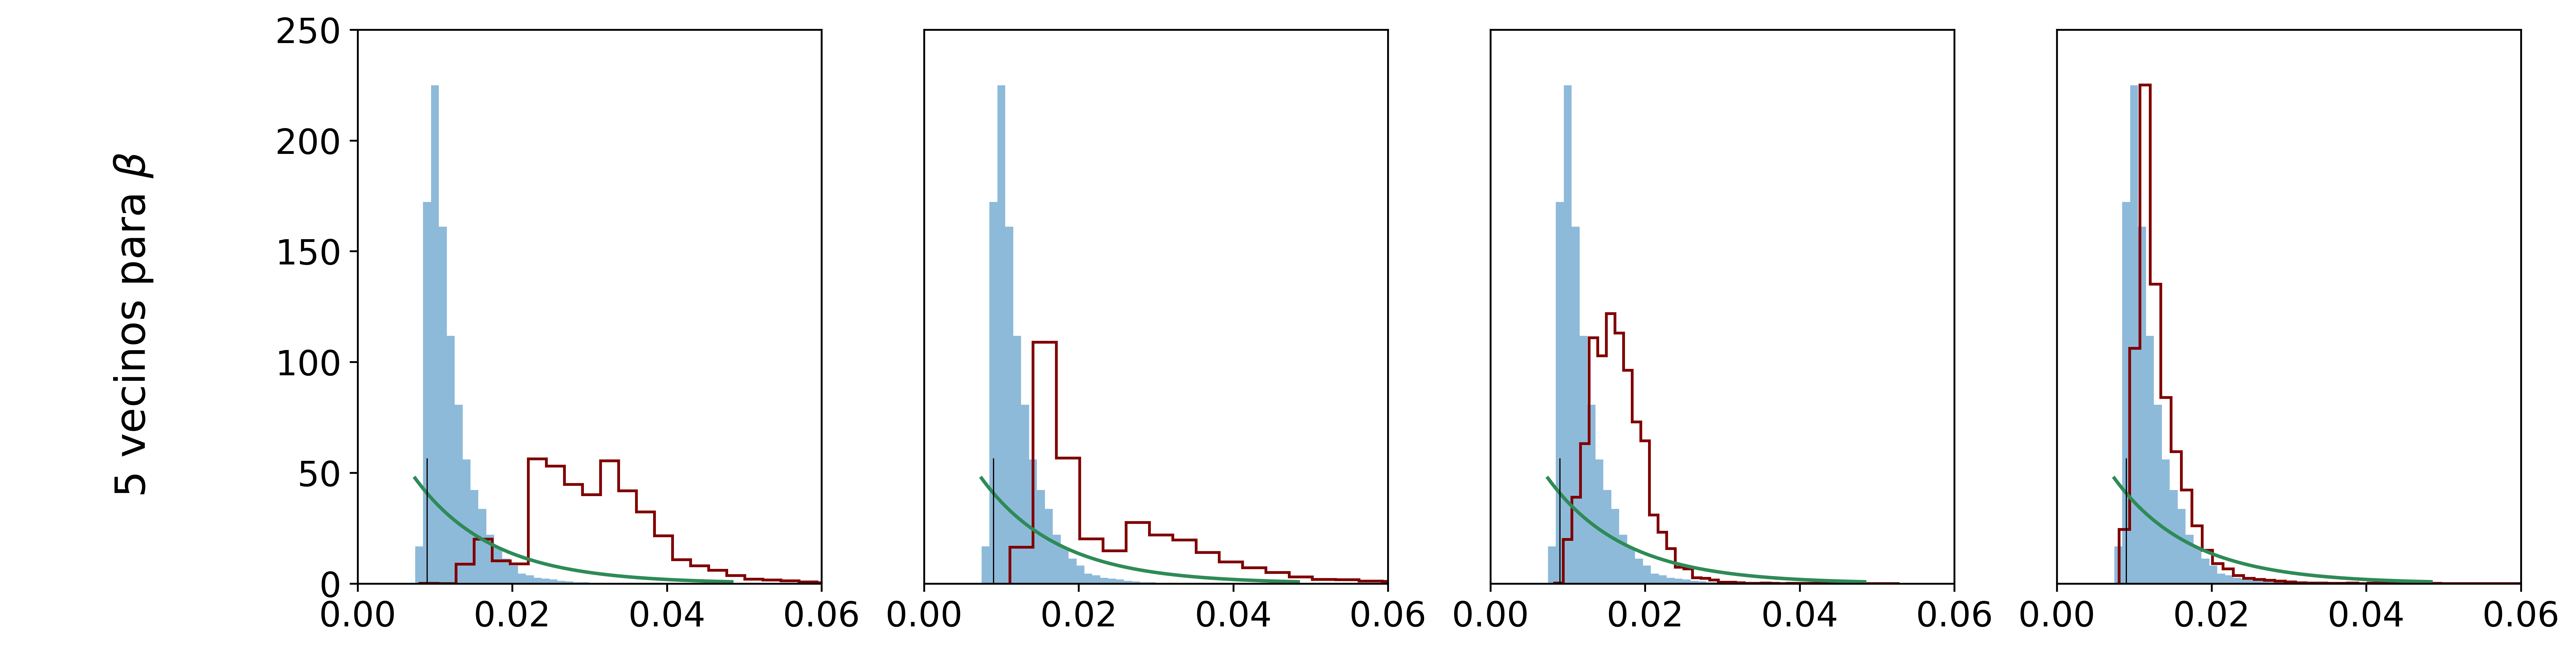
\includegraphics[width = 12 cm ]{img/Unidades_1.png} 
    % \caption{}
    % \label{Fig. }
  \end{figure} 
  \begin{figure}[H] 
    \centering 
    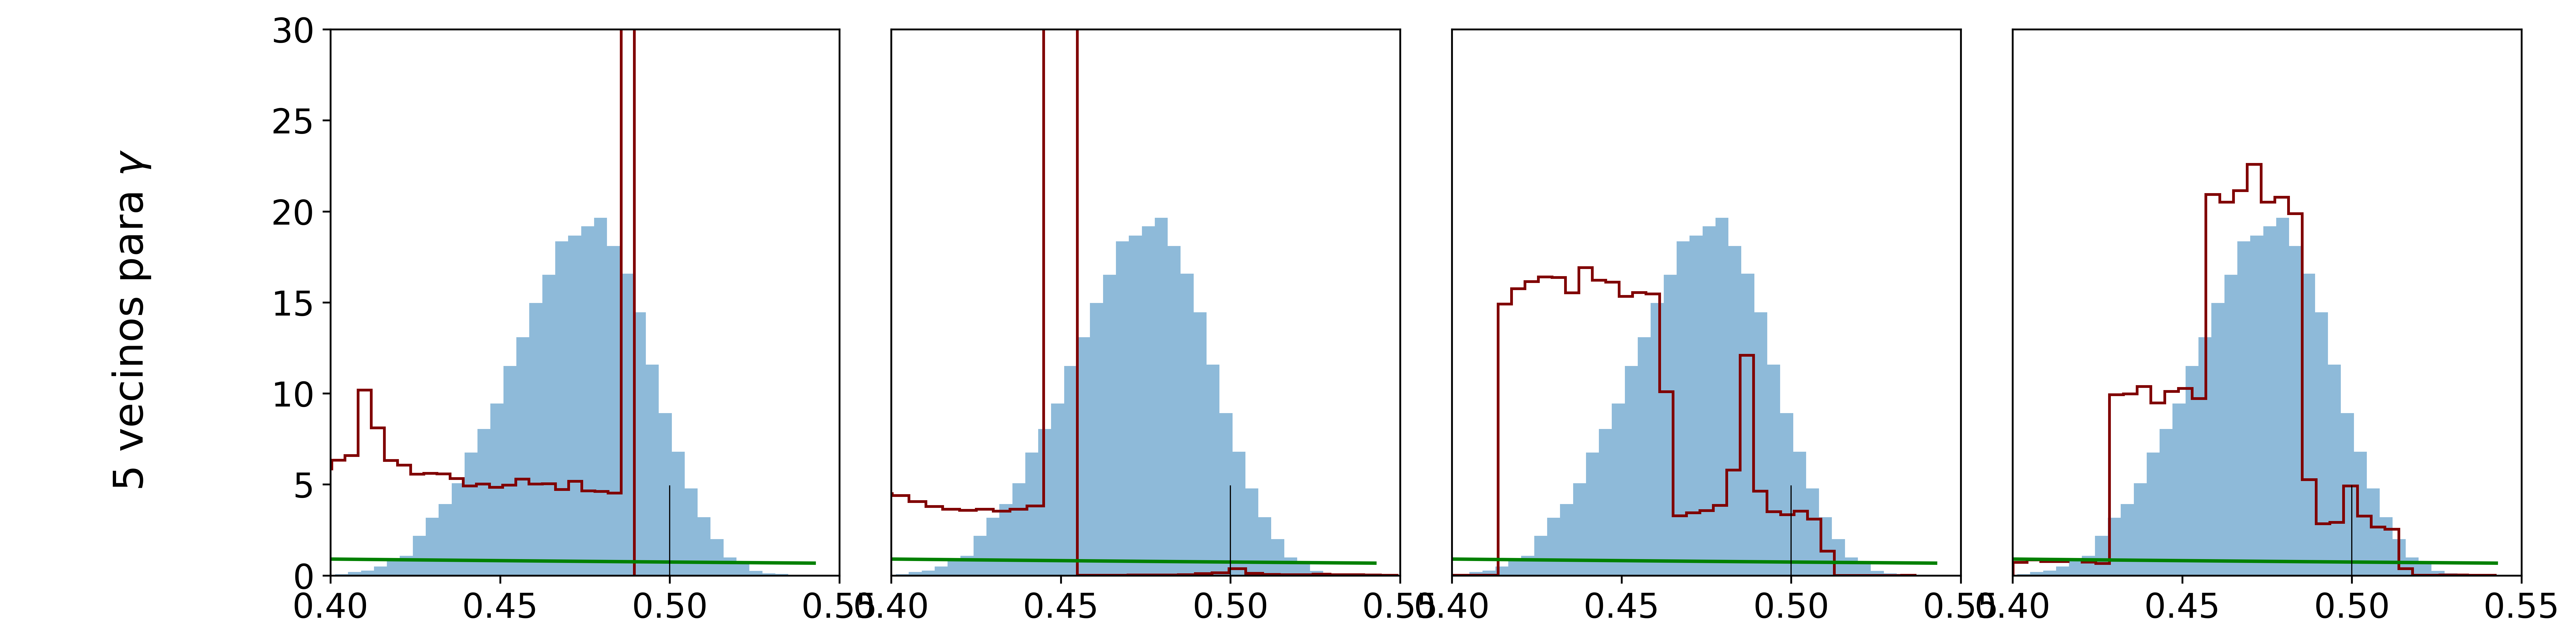
\includegraphics[width = 12 cm ]{img/Unidades_2} 
    % \caption{Distribuciones marginales posteriores aproximadas (rojo) con forward map aproximado a cinco vecinos cercanos y una malla de resolución 10,15,30,50 de izquierda a derecha, sin regularización de las unidades. En azul la distribución posterior con forward map ordinario para modelo SIR.}
    \label{Fig. Regulacion_1}
  \end{figure} 
\end{frame}

\begin{frame}{Conclusiones}
  \begin{figure}[H] 
    \centering 
    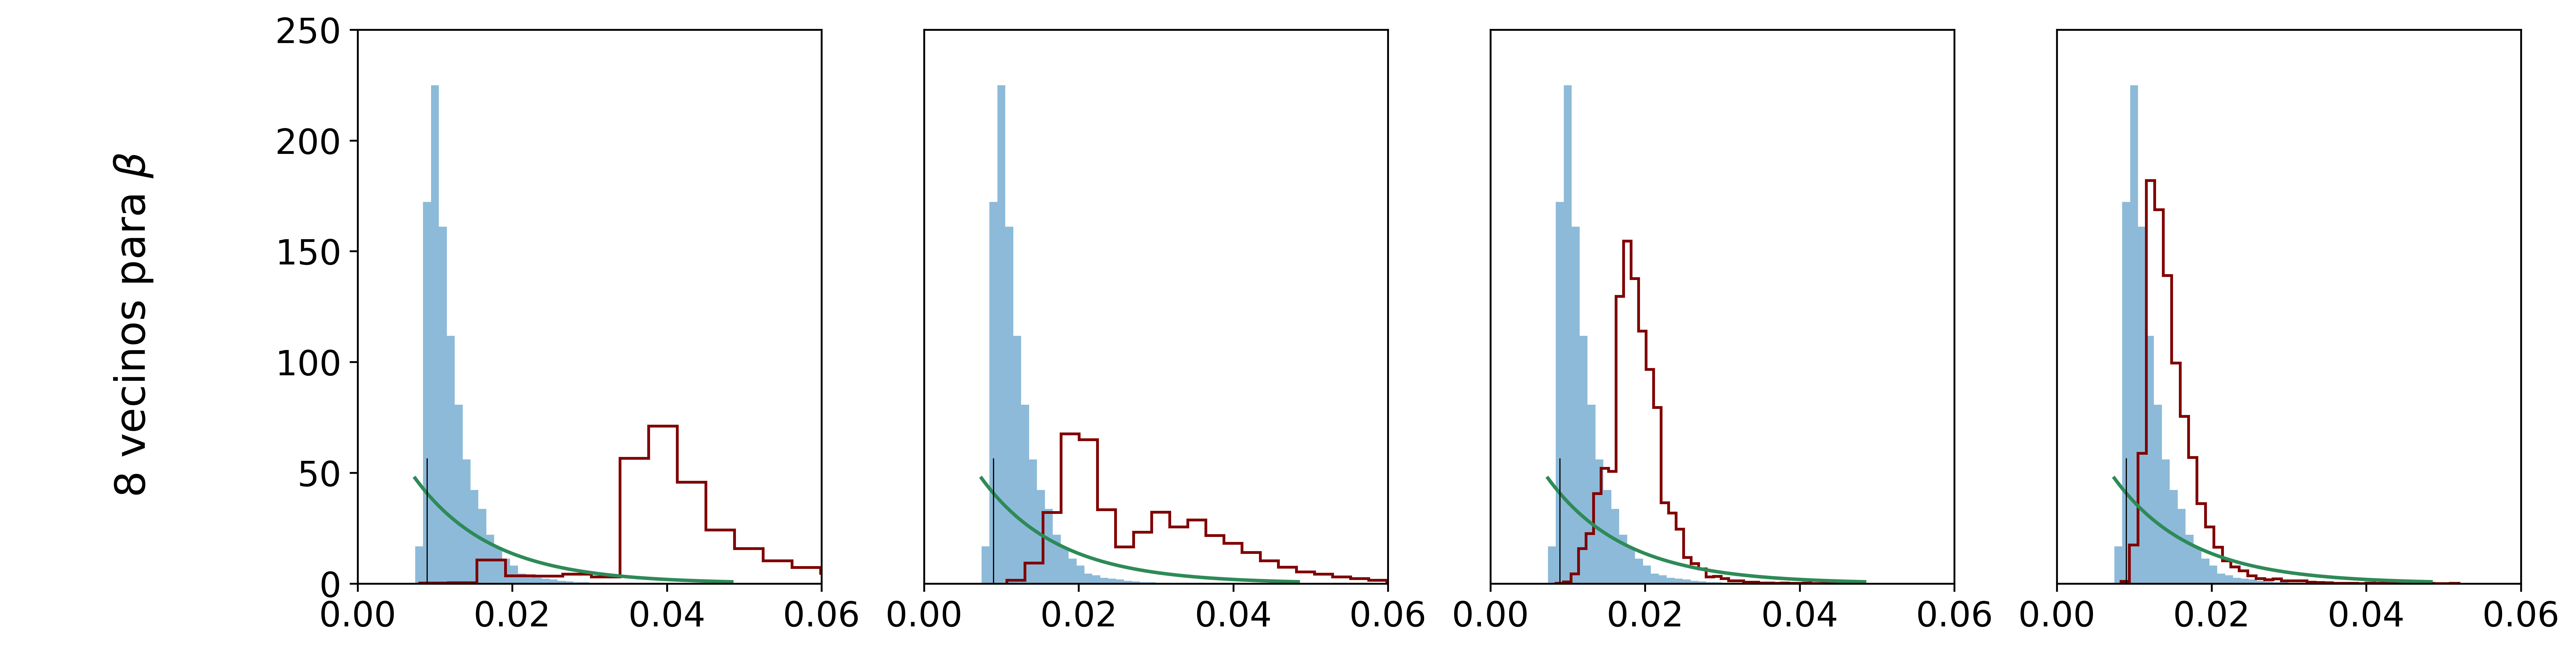
\includegraphics[width = 12 cm ]{img/Unidades_3.png} 
    % \caption{}
    % \label{Fig. }
  \end{figure} 
  \begin{figure}[H] 
    \centering 
    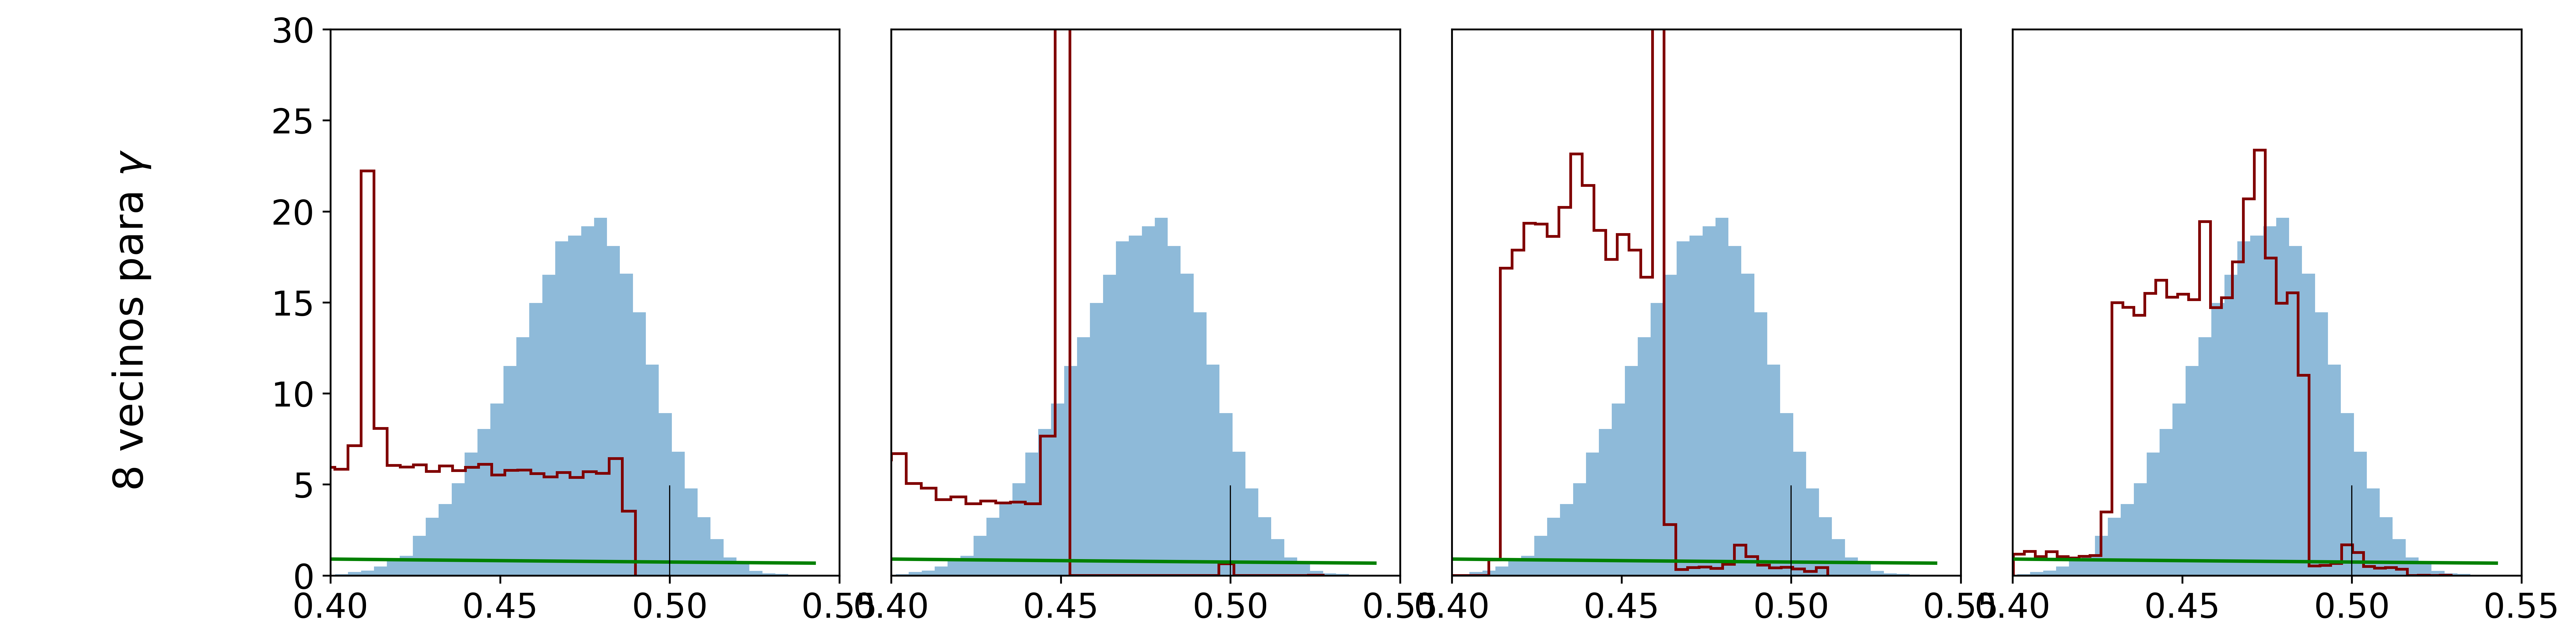
\includegraphics[width = 12 cm ]{img/Unidades_4} 
    % \caption{Distribuciones marginales posteriores aproximadas (rojo) con forward map aproximado a ocho vecinos cercanos y una malla de resolución 10,15,30,50 de izquierda a derecha, sin regularización de las unidades. En azul la distribución posterior con forward map ordinario para modelo SIR.}
    \label{Fig. Regulacion_2}
  \end{figure} 
\end{frame}

\begin{frame}{Trabajo Futuro}
  \begin{itemize}
    \item 
    Existen multiples formas de mejorar el algoritmo para la solución del problema inverso en modelos dados por EDO's. Una de ellas considerada a trabajo futuro es la creación de mallas no rectangulares, que además se vaya construyendo de forma adaptativa.

    \vspace{0.5 cm}

    \item Investigar el comportamiento anómalo en las distintas ejecuciones de los experimentos realizados.

    \vspace{0.5 cm}

    \item También considerado a futuro, es de interés trabajar con distintos modelos de EDO's a los presentados en este proyecto, pues de esta forma se podrían encontrar casos en los que la metodología aproximada propuesta aquí resulte con irregularidades, donde el tratamiento de estas conlleve a la mejora del algoritmo.
  \end{itemize}
\end{frame}


\begin{frame}{Referencias}

  \begin{figure}[H] 
    \centering 
    \includegraphics[width = 14 cm ]{Figures/Referencias.png} 
  \end{figure} 

\end{frame}

\section{Material Extra}


\begin{frame}{Simulación del Modelo Logístico}
  \begin{figure}
    \centering 
    \includegraphics[width = 9 cm ]{img/Exp_Central_logistico_sigma/Figuras/Generales/Muestra_logistico_sigma.png} 
    % \caption{Muestra $\mathbf{y}$ para el modelo logístico.}
    \label{Fig. 3.2.log.muestra}
  \end{figure} 
\end{frame}


\begin{frame}{Simulación del Modelo Logístico}
  \begin{figure} 
    \centering 
    \includegraphics[width = 15 cm]{img/Exp_Central_logistico_sigma/Figuras/Generales/Apriori_logistico_sigma.png}     
    % \caption{Distribuciones a priori para $\theta_1$ y $\theta_2$}
    \label{Fig. 3.2.log.priori}
  \end{figure} 
\end{frame}


\begin{frame}{Simulación del Modelo Logístico}
  \begin{figure}
    \centering 
    \includegraphics[width = 10 cm ]{img/Exp_Central_logistico_sigma/Figuras/Generales/Conjunta_logistico_sigma.png} 
    \caption{Posterior conjunta para el modelo logístico.}
    \label{Fig. 3.2.log.conjunta}
  \end{figure} 
\end{frame}


\begin{frame}{Simulación del Modelo Logístico}
  \begin{columns}[T,onlytextwidth]
    \column{0.5\textwidth}
    
    \begin{figure}
      \centering 
      \includegraphics[width=0.9\textwidth]{img/Exp_Central_logistico_sigma/Figuras/Generales/Post_theta1_logistico_sigma.png}
    \end{figure} 
    
    \column{0.5\textwidth}
    
      % \metroset{block=fill}
      
    \begin{figure}
      \centering 
      \includegraphics[width=0.9\textwidth]{img/Exp_Central_logistico_sigma/Figuras/Generales/Post_theta2_logistico_sigma.png}
    \end{figure} 
    
  \end{columns}
\end{frame}


\begin{frame}{Simulación del Modelo Logístico}
  \begin{figure}
    \centering 
    \includegraphics[width = 10 cm ]{img/Exp_Central_logistico_sigma/Figuras/Generales/Predictiva_logistico_sigma.png} 
    % \caption{Distribución predictiva para el modelo logístico.}
    \label{Fig. 3.2.log.predictiva}
  \end{figure} 
\end{frame}


\begin{frame}{Simulación del Modelo SIR}
  \begin{figure}
    \centering 
    \includegraphics[width = 10 cm]{img/Exp_Central_SIR_sigma/Figuras/Generales/Muestra_SIR_sigma.png} 
    % \caption{Muestra $\mathbf{y}$ del modelo SIR.}
    \label{Fig. SIR_01}
  \end{figure} 
\end{frame}

\begin{frame}{Simulación del Modelo SIR}
  \begin{figure}[H] 
    \centering 
    \includegraphics[width = 12 cm ]{img/Exp_Central_SIR_sigma/Figuras/Generales/Apriori_SIR_sigma.png} 
    % \caption{Distribuciones marginal a priori para el parámetro $\beta$ (izquierda) y $\gamma$ (derecha).}
    \label{Fig. SIR_02}
  \end{figure} 
\end{frame}



\begin{frame}{Simulación del Modelo SIR}
  \begin{figure}[H] 
    \centering 
    \includegraphics[width = 9 cm]{img/Exp_Central_SIR_sigma/Figuras/Generales/Conjunta_SIR_sigma.png} 
    % \caption{Distribución posterior conjunta para el modelo SIR.}
    \label{Fig. SIR_03}
  \end{figure} 
\end{frame}

\begin{frame}{Simulación del Modelo SIR}
  \begin{columns}[T,onlytextwidth]
    \column{0.5\textwidth}
    
    \begin{figure}
      \centering 
      \includegraphics[width=0.9\textwidth]{img/Exp_Central_SIR_sigma/Figuras/Generales/Post_theta1_SIR_sigma.png}
    \end{figure} 
    
    \column{0.5\textwidth}
    
      % \metroset{block=fill}
      
    \begin{figure}
      \centering 
      \includegraphics[width=0.9\textwidth]{img/Exp_Central_SIR_sigma/Figuras/Generales/Post_theta2_SIR_sigma.png}
    \end{figure} 
    
  \end{columns}
\end{frame}

\begin{frame}{Simulación del Modelo SIR}
  
  \begin{figure}[H] 
    \centering 
    \includegraphics[width = 10 cm ]{img/Exp_Central_SIR_sigma/Figuras/Generales/Predictiva_SIR_sigma.png} 
    % \caption{Distribución predictiva para el modelo SIR.}
    \label{Fig. SIR_06}
  \end{figure} 
\end{frame}













% \begin{frame}[fragile]{Forward map}
  
%   \textbf{El problema directo:}
  
%   Predecir los valores de las observables físicos $\mathbf{d}$ que corresponde a un modelo $\boldsymbol{\theta}$
%   \begin{align*}
%       \boldsymbol{\theta} \:\:\:\:\: \mapsto \:\:\:\:\: \mathbf{d} = \mathbf{F(\boldsymbol{\theta})}
%   \end{align*}


%   \vspace*{1 cm}

%   Incertidumbre de las mediciones e imperfecciones del modelo \cite{tarantola2005inverse}. 

% \end{frame}


% \begin{frame}{Ejemplos}
%   \begin{columns}[T,onlytextwidth]
%     \column{0.5\textwidth}

    
%     \begin{alertblock}{Resorte sujeto a fricción}
%       Sea $x(t)$ la posición
%       \begin{align*}
%         m\ddot{x} = -kx + b \dot{x}
%       \end{align*}
%     \end{alertblock}
    
%     \begin{block}{Caída sujeto a fricción}
%       Sea $x(t)$ la posición
%       \begin{align*}
%         m\ddot{x} = g - b \dot{x}
%       \end{align*}
%           % $x(0) = \dot{x(0)} = 0$.
%     \end{block}

%       \begin{alertblock}{Crecimiento poblacional}
%         Sea $P(t)$ el tamaño de población
%         \begin{align*}
%           \frac{dP}{dt} = r P \left(1 - \frac{P}{K}\right) 
%         \end{align*}
%       \end{alertblock}

%     \column{0.5\textwidth}

%       \metroset{block=fill}

%       \begin{alertblock}{Forward map}
%         $\theta = (k,b)  \:\:\: \mapsto \:\:\: F(\theta) = x(t)$
%       \end{alertblock}
      
%       \vspace*{1 cm}
      
%       \begin{block}{Forward map}
%         $\theta = (g,b)  \:\:\: \mapsto \:\:\: F(\theta) = x(t)$
%       \end{block}

%       \vspace*{1 cm}

%       \begin{alertblock}{Forward map}
%         $\theta = (r,K)  \:\:\: \mapsto \:\:\: F(\theta) = P(t)$
%       \end{alertblock}

%   \end{columns}
% \end{frame}

% \begin{frame}[fragile]{Estadística bayesiana}
  
%   La distribución posterior 
%   \begin{align*}
%       \pi(\theta|x^n) &\propto \mathcal{L}(\theta|x^n) \pi(\theta)
%   \end{align*}
  

% \begin{figure}[H] 
%     \centering 
%     \includegraphics[width = 5.50 cm]{Figures/bayes1.png} 
%     % \caption{}
%     % \label{Fig. }
% \end{figure} 




% \end{frame}

% \begin{frame}[fragile]{Incertidumbre en los errores}
%   Procedimiento:
%   \begin{itemize}
%     \item 
%     \textbf{Observaciones:} $(x_1, t_1), (x_2,t_2), \cdots, (x_n, t_n)$ 
%     \item 
%     Cuantificar el error mediante la relación
%     \begin{align*}
%         x_i = F_\theta (t_i) + \varepsilon_i, \:\:\:\:\: i = 1,...,n
%     \end{align*}
%     \item Un supuesto convencional sobre los errores
%     \begin{align*}
%         \varepsilon_i \sim N(0,\sigma^2)
%         \label{3.02}
%     \end{align*}

%   \end{itemize}

% \end{frame}

% \begin{frame}[fragile]{Inferencia}
  
%   Distribución posterior 
%   \begin{align*}
%       \pi(\theta|x^n) &\propto \mathcal{L}(\theta|x^n) \pi_{\Theta}(\theta)\\
%       & \left[\propto \prod_{i=1}^n \frac{1}{\sqrt{2\pi \sigma^2}} exp \left({-\frac{1}{2\sigma^2}\left(x_i - F_{\theta}(t_i)\right)^2 }\right)\right] \pi_{\Theta}(\theta) \\
%       & \propto \left(\frac{1}{2\pi\sigma^2}\right)^{n/2} exp {\left(\frac{1}{2\sigma^2} \sum_{i =1}^{n}\left(x_i - F_{\theta}(t_i)\right) ^2\right) } \pi_{\Theta}(\theta)
%   \end{align*}
%   donde $\theta = (\theta_1, ..., \theta_m)$.
  
%   \vspace{1 cm}

%   \textbf{Simular por métodos Monte Carlo}
%   \begin{itemize}
%     \item 
%     Se simula por MCMC Metropolis-Hastings \cite{robert1999monte}.
%   \end{itemize}


%   % Es posible simular variables aleatorias con dicha distribución y así obtener estimaciones de los parámetros del modelo.
% \end{frame}




% \section{Ejemplo}


% \begin{frame}{Resorte sujeto a fricción}
%   \begin{figure}
%       \centering 
%       \includegraphics[width = 10cm]{Figures/0.png} 
%       % \caption{}
%       % \label{Fig. }
%   \end{figure} 
% \end{frame}

% \begin{frame}
%   \begin{figure}
%       \centering 
%       \includegraphics[width = 10 cm]{Figures/1.png} 
%       % \caption{}
%       % \label{Fig. }
%   \end{figure} 
% \end{frame}

% \begin{frame}
%   \begin{figure}[H] 
%       \centering 
%       \includegraphics[width = 10 cm]{Figures/2.png} 
%       % \caption{}
%       % \label{Fig. }
%   \end{figure} 
% \end{frame}

% \begin{frame}
%   \begin{figure}[H] 
%       \centering 
%       \includegraphics[width = 10 cm]{Figures/3.png} 
%       % \caption{}
%       % \label{Fig. }
%   \end{figure} 
% \end{frame}


% \begin{frame}
%   \begin{figure}[H] 
%       \centering 
%       \includegraphics[width = 10 cm]{Figures/4.png} 
%       % \caption{}
%       % \label{Fig. }
%   \end{figure} 
% \end{frame}



% \section{Objetivos}


% \begin{frame}{Objetivos}
%   A pesar de que el análisis previo nos permite obtener estimaciones bastante precisas para el problema inverso. Sin embargo, son \textbf{computacionalmente pesadas}, esto debido a que a cada paso en la cadena requiere que se solucione el problema forward, es decir, se resuelven ecuaciones diferenciales tantas veces como se deje correr la cadena. 
%   \begin{itemize}
%     \item 
%     Se desea encontrar una especie de \textit{interpolación} para solo solucionar una cantidad pequeña de veces el problema forward y para cada punto en el espacio de parámetros se pueda aproximar la solución en función de las soluciones con parámetros cercanos.
%   \end{itemize}

% \end{frame}

% \begin{frame}
%   \begin{figure}[H] 
%       \centering 
%       \includegraphics[width = 10 cm]{Figures/5.png} 
%       % \caption{}
%       % \label{Fig. }
%   \end{figure} 
% \end{frame}











% \section{Plan de trabajo}

% \begin{frame}{Plan de trabajo}
  
%   \begin{figure}[H] 
%       \centering 
%       \includegraphics[width = 14 cm]{Figures/cronograma.png} 
%       % \caption{}
%       % \label{Fig. }
%   \end{figure} 
% \end{frame}



\begin{frame}{Referencias}

  \bibliography{demo}
  \bibliographystyle{abbrv}

\end{frame}



% \begin{frame}{Referencias}

  
% \end{frame}












\end{document}
